% Options for packages loaded elsewhere
\PassOptionsToPackage{unicode}{hyperref}
\PassOptionsToPackage{hyphens}{url}
%
\documentclass[
]{book}
\usepackage{amsmath,amssymb}
\usepackage{lmodern}
\usepackage{iftex}
\ifPDFTeX
  \usepackage[T1]{fontenc}
  \usepackage[utf8]{inputenc}
  \usepackage{textcomp} % provide euro and other symbols
\else % if luatex or xetex
  \usepackage{unicode-math}
  \defaultfontfeatures{Scale=MatchLowercase}
  \defaultfontfeatures[\rmfamily]{Ligatures=TeX,Scale=1}
\fi
% Use upquote if available, for straight quotes in verbatim environments
\IfFileExists{upquote.sty}{\usepackage{upquote}}{}
\IfFileExists{microtype.sty}{% use microtype if available
  \usepackage[]{microtype}
  \UseMicrotypeSet[protrusion]{basicmath} % disable protrusion for tt fonts
}{}
\makeatletter
\@ifundefined{KOMAClassName}{% if non-KOMA class
  \IfFileExists{parskip.sty}{%
    \usepackage{parskip}
  }{% else
    \setlength{\parindent}{0pt}
    \setlength{\parskip}{6pt plus 2pt minus 1pt}}
}{% if KOMA class
  \KOMAoptions{parskip=half}}
\makeatother
\usepackage{xcolor}
\usepackage{color}
\usepackage{fancyvrb}
\newcommand{\VerbBar}{|}
\newcommand{\VERB}{\Verb[commandchars=\\\{\}]}
\DefineVerbatimEnvironment{Highlighting}{Verbatim}{commandchars=\\\{\}}
% Add ',fontsize=\small' for more characters per line
\usepackage{framed}
\definecolor{shadecolor}{RGB}{248,248,248}
\newenvironment{Shaded}{\begin{snugshade}}{\end{snugshade}}
\newcommand{\AlertTok}[1]{\textcolor[rgb]{0.94,0.16,0.16}{#1}}
\newcommand{\AnnotationTok}[1]{\textcolor[rgb]{0.56,0.35,0.01}{\textbf{\textit{#1}}}}
\newcommand{\AttributeTok}[1]{\textcolor[rgb]{0.77,0.63,0.00}{#1}}
\newcommand{\BaseNTok}[1]{\textcolor[rgb]{0.00,0.00,0.81}{#1}}
\newcommand{\BuiltInTok}[1]{#1}
\newcommand{\CharTok}[1]{\textcolor[rgb]{0.31,0.60,0.02}{#1}}
\newcommand{\CommentTok}[1]{\textcolor[rgb]{0.56,0.35,0.01}{\textit{#1}}}
\newcommand{\CommentVarTok}[1]{\textcolor[rgb]{0.56,0.35,0.01}{\textbf{\textit{#1}}}}
\newcommand{\ConstantTok}[1]{\textcolor[rgb]{0.00,0.00,0.00}{#1}}
\newcommand{\ControlFlowTok}[1]{\textcolor[rgb]{0.13,0.29,0.53}{\textbf{#1}}}
\newcommand{\DataTypeTok}[1]{\textcolor[rgb]{0.13,0.29,0.53}{#1}}
\newcommand{\DecValTok}[1]{\textcolor[rgb]{0.00,0.00,0.81}{#1}}
\newcommand{\DocumentationTok}[1]{\textcolor[rgb]{0.56,0.35,0.01}{\textbf{\textit{#1}}}}
\newcommand{\ErrorTok}[1]{\textcolor[rgb]{0.64,0.00,0.00}{\textbf{#1}}}
\newcommand{\ExtensionTok}[1]{#1}
\newcommand{\FloatTok}[1]{\textcolor[rgb]{0.00,0.00,0.81}{#1}}
\newcommand{\FunctionTok}[1]{\textcolor[rgb]{0.00,0.00,0.00}{#1}}
\newcommand{\ImportTok}[1]{#1}
\newcommand{\InformationTok}[1]{\textcolor[rgb]{0.56,0.35,0.01}{\textbf{\textit{#1}}}}
\newcommand{\KeywordTok}[1]{\textcolor[rgb]{0.13,0.29,0.53}{\textbf{#1}}}
\newcommand{\NormalTok}[1]{#1}
\newcommand{\OperatorTok}[1]{\textcolor[rgb]{0.81,0.36,0.00}{\textbf{#1}}}
\newcommand{\OtherTok}[1]{\textcolor[rgb]{0.56,0.35,0.01}{#1}}
\newcommand{\PreprocessorTok}[1]{\textcolor[rgb]{0.56,0.35,0.01}{\textit{#1}}}
\newcommand{\RegionMarkerTok}[1]{#1}
\newcommand{\SpecialCharTok}[1]{\textcolor[rgb]{0.00,0.00,0.00}{#1}}
\newcommand{\SpecialStringTok}[1]{\textcolor[rgb]{0.31,0.60,0.02}{#1}}
\newcommand{\StringTok}[1]{\textcolor[rgb]{0.31,0.60,0.02}{#1}}
\newcommand{\VariableTok}[1]{\textcolor[rgb]{0.00,0.00,0.00}{#1}}
\newcommand{\VerbatimStringTok}[1]{\textcolor[rgb]{0.31,0.60,0.02}{#1}}
\newcommand{\WarningTok}[1]{\textcolor[rgb]{0.56,0.35,0.01}{\textbf{\textit{#1}}}}
\usepackage{longtable,booktabs,array}
\usepackage{calc} % for calculating minipage widths
% Correct order of tables after \paragraph or \subparagraph
\usepackage{etoolbox}
\makeatletter
\patchcmd\longtable{\par}{\if@noskipsec\mbox{}\fi\par}{}{}
\makeatother
% Allow footnotes in longtable head/foot
\IfFileExists{footnotehyper.sty}{\usepackage{footnotehyper}}{\usepackage{footnote}}
\makesavenoteenv{longtable}
\usepackage{graphicx}
\makeatletter
\def\maxwidth{\ifdim\Gin@nat@width>\linewidth\linewidth\else\Gin@nat@width\fi}
\def\maxheight{\ifdim\Gin@nat@height>\textheight\textheight\else\Gin@nat@height\fi}
\makeatother
% Scale images if necessary, so that they will not overflow the page
% margins by default, and it is still possible to overwrite the defaults
% using explicit options in \includegraphics[width, height, ...]{}
\setkeys{Gin}{width=\maxwidth,height=\maxheight,keepaspectratio}
% Set default figure placement to htbp
\makeatletter
\def\fps@figure{htbp}
\makeatother
\setlength{\emergencystretch}{3em} % prevent overfull lines
\providecommand{\tightlist}{%
  \setlength{\itemsep}{0pt}\setlength{\parskip}{0pt}}
\setcounter{secnumdepth}{5}
\usepackage{booktabs}
\usepackage{amsthm}
\makeatletter
\def\thm@space@setup{%
  \thm@preskip=8pt plus 2pt minus 4pt
  \thm@postskip=\thm@preskip
}
\makeatother
\ifLuaTeX
  \usepackage{selnolig}  % disable illegal ligatures
\fi
\usepackage[]{natbib}
\bibliographystyle{apalike}
\IfFileExists{bookmark.sty}{\usepackage{bookmark}}{\usepackage{hyperref}}
\IfFileExists{xurl.sty}{\usepackage{xurl}}{} % add URL line breaks if available
\urlstyle{same} % disable monospaced font for URLs
\hypersetup{
  pdftitle={Applied Spatial Data Analysis - Spatial Point and Lattice Data},
  pdfauthor={Dr Sebnem Er},
  hidelinks,
  pdfcreator={LaTeX via pandoc}}

\title{Applied Spatial Data Analysis - Spatial Point and Lattice Data}
\author{Dr Sebnem Er}
\date{2023-02-21}

\begin{document}
\maketitle

{
\setcounter{tocdepth}{1}
\tableofcontents
}
\hypertarget{introduction}{%
\chapter{Introduction}\label{introduction}}

This book will guide you through the R codes for Spatial Point and Lattice Data Analysis.

The chapters will be made available on Tuesdays when we start a new week So please update your browser to access the codes for the relevant chapter.

\hypertarget{spatial-point-pattern-analysis}{%
\chapter{Spatial Point Pattern Analysis}\label{spatial-point-pattern-analysis}}

\hypertarget{prerequisites}{%
\section{Prerequisites}\label{prerequisites}}

You need to have the following R packages installed and recalled into your library:

\begin{Shaded}
\begin{Highlighting}[]
\FunctionTok{suppressPackageStartupMessages}\NormalTok{(\{}
\FunctionTok{library}\NormalTok{(sf)}
\FunctionTok{library}\NormalTok{(spatstat)}
\FunctionTok{library}\NormalTok{(spatstat.data)}
\FunctionTok{library}\NormalTok{(ggplot2)}
\FunctionTok{library}\NormalTok{(sp)}
\FunctionTok{library}\NormalTok{(animation)}
\FunctionTok{library}\NormalTok{(plotrix)}
\FunctionTok{library}\NormalTok{(tmap)\})}
\end{Highlighting}
\end{Shaded}

\hypertarget{datasets---readily-available-imported-simulated-datasets}{%
\section{Datasets - Readily Available, Imported, Simulated Datasets}\label{datasets---readily-available-imported-simulated-datasets}}

\hypertarget{simple-feature-basics}{%
\subsection{Simple Feature Basics}\label{simple-feature-basics}}

\begin{Shaded}
\begin{Highlighting}[]
\FunctionTok{library}\NormalTok{(sf)}
\end{Highlighting}
\end{Shaded}

\texttt{sf} geometry types:

\begin{itemize}
\tightlist
\item
  point: \texttt{st\_point()}
\item
  linestring: \texttt{st\_linestring()}
\item
  polygon: \texttt{st\_polygon()}
\item
  multipoint: \texttt{st\_multipoint()}
\item
  multilinestring: \texttt{st\_multilinestring()}
\item
  multipolygon: \texttt{st\_multipolygon()}
\item
  collection of different geometry types: \texttt{st\_geometrycollection()}
\end{itemize}

\hypertarget{sfg}{%
\subsubsection{sfg}\label{sfg}}

\begin{itemize}
\tightlist
\item
  A single \texttt{point} and \texttt{multipoint}
\end{itemize}

\begin{Shaded}
\begin{Highlighting}[]
\CommentTok{\# Using the sf library for simple features}

\CommentTok{\# Tarih      Saat      Enlem(N)  Boylam(E) Derinlik(km)  MD   ML   Mw    Yer                                             Çözüm Niteliği}
\CommentTok{\# {-}{-}{-}{-}{-}{-}{-}{-}{-}{-} {-}{-}{-}{-}{-}{-}{-}{-}  {-}{-}{-}{-}{-}{-}{-}{-}  {-}{-}{-}{-}{-}{-}{-}   {-}{-}{-}{-}{-}{-}{-}{-}{-}{-}    {-}{-}{-}{-}{-}{-}{-}{-}{-}{-}{-}{-}    {-}{-}{-}{-}{-}{-}{-}{-}{-}{-}{-}{-}{-}{-}                                  {-}{-}{-}{-}{-}{-}{-}{-}{-}{-}{-}{-}{-}{-}}
\CommentTok{\# 2023.02.15 14:46:46  36.8803   36.6177        8.3      {-}.{-}  2.8  {-}.{-}   ASAGIBILENLER{-}ISLAHIYE (GAZIANTEP)                }
\CommentTok{\# 2023.02.15 14:43:05  37.0218   28.8915        8.4      {-}.{-}  2.7  {-}.{-}   OTMANLAR{-}KOYCEGIZ (MUGLA)}


\CommentTok{\# sf::st\_crs(4326), which means x and y positions are interpreted as longitude (E) and latitude (N), respectively, in the World Geodetic System 1984 (WGS84)}

\NormalTok{point1\_sg }\OtherTok{=} \FunctionTok{c}\NormalTok{(}\FloatTok{36.6177}\NormalTok{, }\FloatTok{36.8803}\NormalTok{) }\SpecialCharTok{\%\textgreater{}\%} \FunctionTok{st\_point}\NormalTok{() }\CommentTok{\# this will create a "sfg" class Geometry}
\FunctionTok{plot}\NormalTok{(point1\_sg)}
\end{Highlighting}
\end{Shaded}

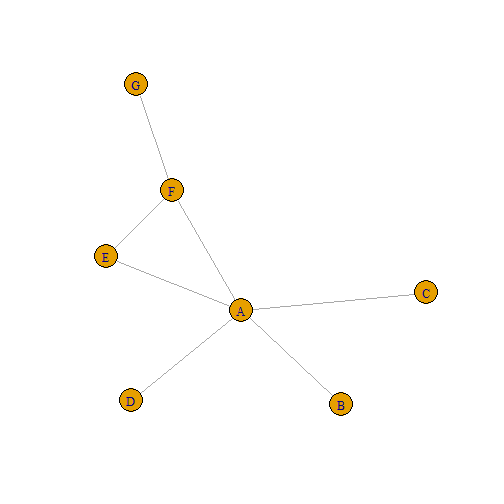
\includegraphics{Applied-Spatial-Data-Analysis_files/figure-latex/unnamed-chunk-3-1.pdf}

\begin{Shaded}
\begin{Highlighting}[]
\FunctionTok{class}\NormalTok{(point1\_sg)}
\end{Highlighting}
\end{Shaded}

\begin{verbatim}
## [1] "XY"    "POINT" "sfg"
\end{verbatim}

\begin{Shaded}
\begin{Highlighting}[]
\NormalTok{point2\_sg }\OtherTok{=} \FunctionTok{c}\NormalTok{(}\FloatTok{28.8915}\NormalTok{, }\FloatTok{37.0218}\NormalTok{) }\SpecialCharTok{\%\textgreater{}\%} \FunctionTok{st\_point}\NormalTok{()}
\FunctionTok{plot}\NormalTok{(point2\_sg)}
\end{Highlighting}
\end{Shaded}

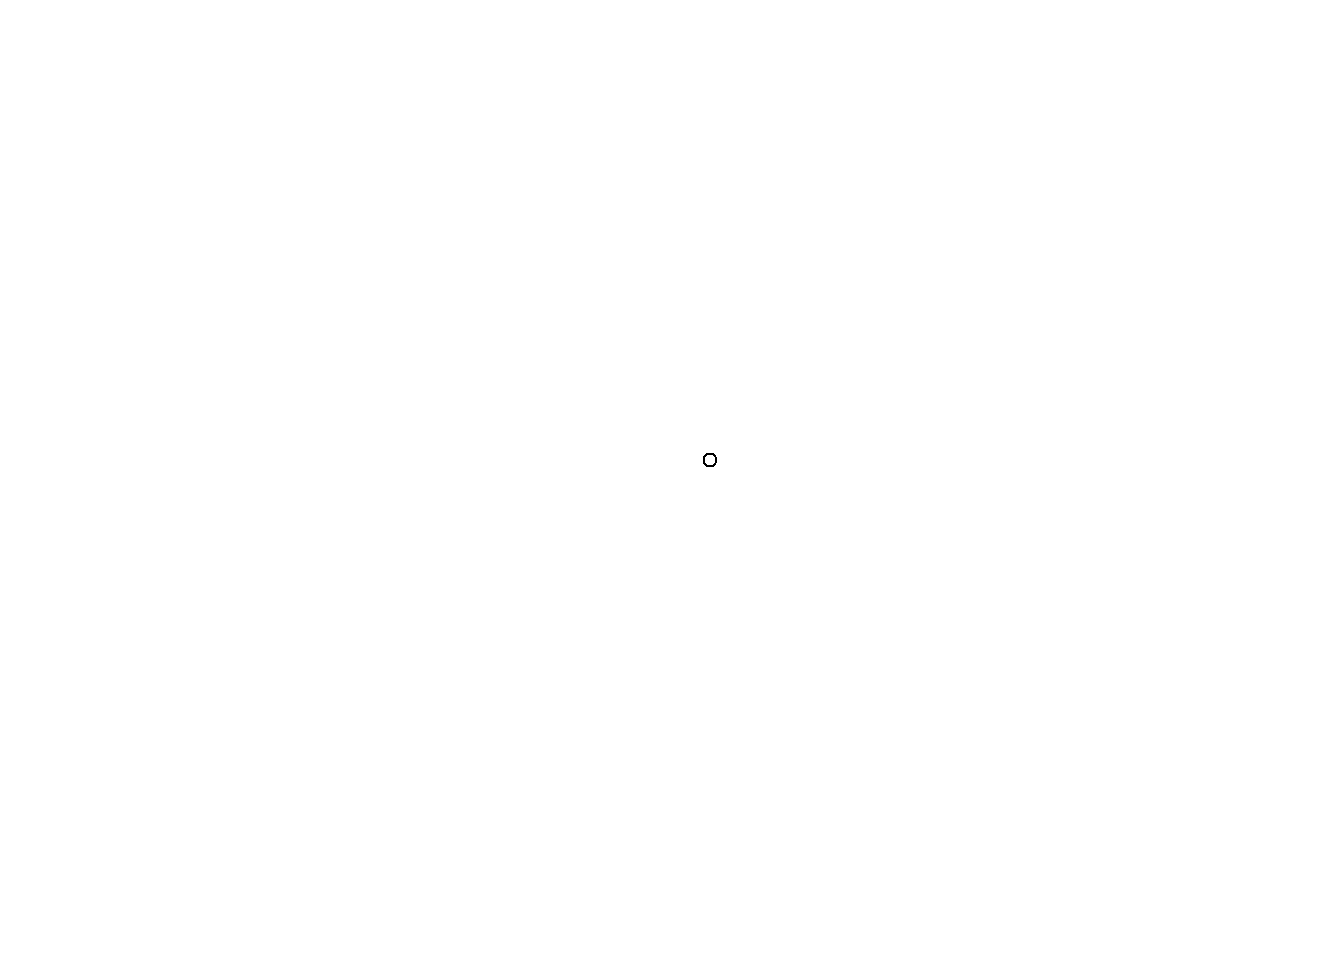
\includegraphics{Applied-Spatial-Data-Analysis_files/figure-latex/unnamed-chunk-3-2.pdf}

\begin{Shaded}
\begin{Highlighting}[]
\FunctionTok{class}\NormalTok{(point2\_sg)}
\end{Highlighting}
\end{Shaded}

\begin{verbatim}
## [1] "XY"    "POINT" "sfg"
\end{verbatim}

\begin{Shaded}
\begin{Highlighting}[]
\NormalTok{points\_sg }\OtherTok{=} \FunctionTok{rbind}\NormalTok{(}\FunctionTok{c}\NormalTok{(}\FloatTok{36.6177}\NormalTok{, }\FloatTok{36.8803}\NormalTok{),}\FunctionTok{c}\NormalTok{(}\FloatTok{28.8915}\NormalTok{, }\FloatTok{37.0218}\NormalTok{)) }\SpecialCharTok{\%\textgreater{}\%} \FunctionTok{st\_multipoint}\NormalTok{()}
\FunctionTok{plot}\NormalTok{(points\_sg)}
\end{Highlighting}
\end{Shaded}

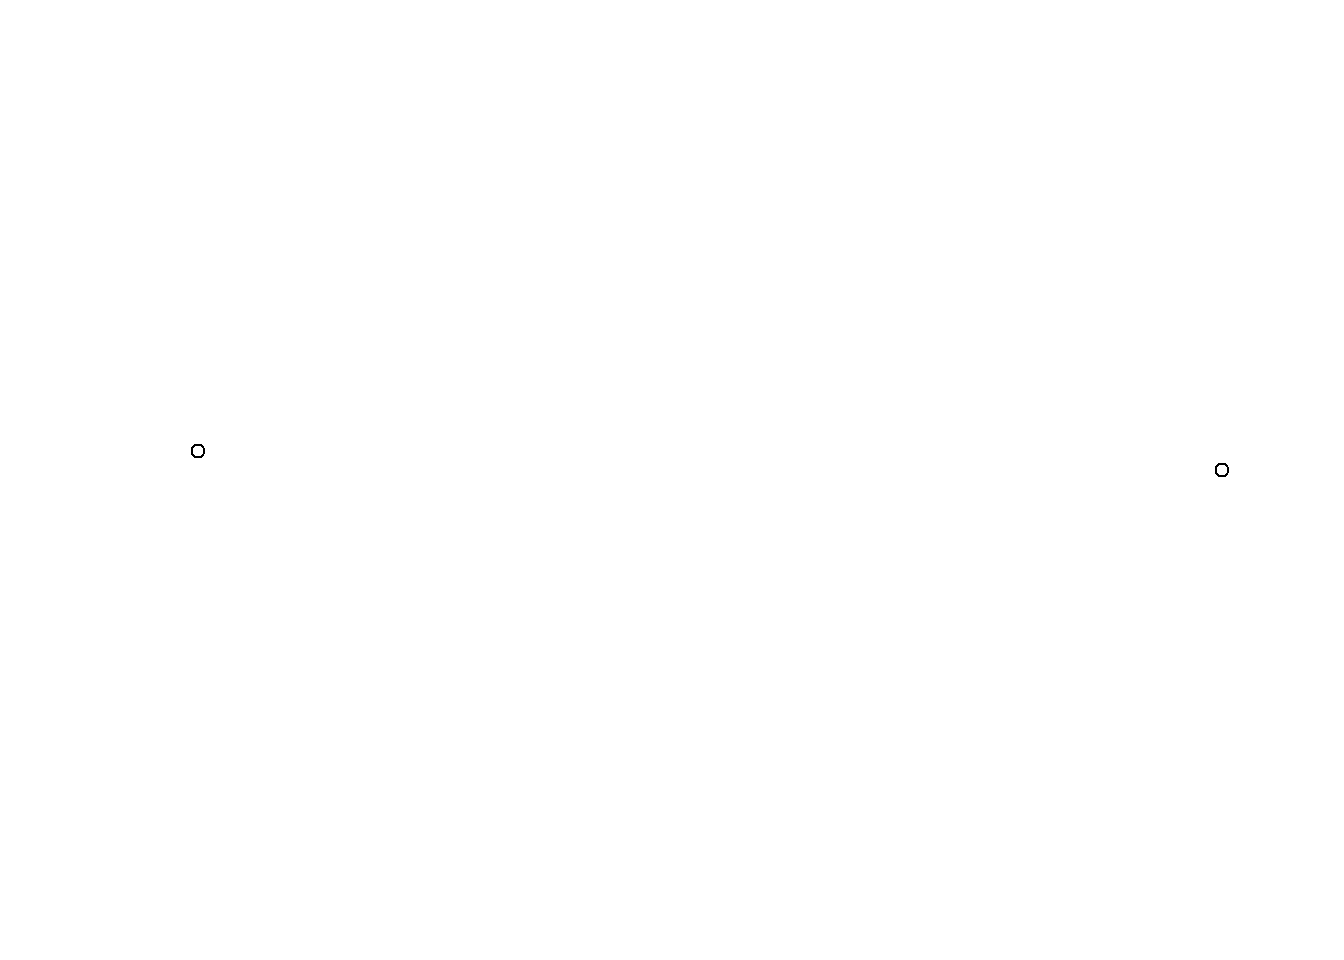
\includegraphics{Applied-Spatial-Data-Analysis_files/figure-latex/unnamed-chunk-3-3.pdf}

\begin{Shaded}
\begin{Highlighting}[]
\FunctionTok{class}\NormalTok{(points\_sg)}
\end{Highlighting}
\end{Shaded}

\begin{verbatim}
## [1] "XY"         "MULTIPOINT" "sfg"
\end{verbatim}

\begin{Shaded}
\begin{Highlighting}[]
\FunctionTok{st\_crs}\NormalTok{(points\_sg)}
\end{Highlighting}
\end{Shaded}

\begin{verbatim}
## Coordinate Reference System: NA
\end{verbatim}

\begin{itemize}
\tightlist
\item
  A single \texttt{polygon} and a \texttt{multipolygon}
\end{itemize}

\begin{Shaded}
\begin{Highlighting}[]
\CommentTok{\# polygon}
\NormalTok{poly1 }\OtherTok{=} \FunctionTok{list}\NormalTok{(}\FunctionTok{rbind}\NormalTok{(}\FunctionTok{c}\NormalTok{(}\FloatTok{35.8337398}\NormalTok{, }\FloatTok{37.8864154}\NormalTok{), }
                   \FunctionTok{c}\NormalTok{(}\FloatTok{36.3281246}\NormalTok{, }\FloatTok{36.7682256}\NormalTok{),}
                   \FunctionTok{c}\NormalTok{(}\FloatTok{38.5803218}\NormalTok{, }\FloatTok{37.7562395}\NormalTok{), }
                   \FunctionTok{c}\NormalTok{(}\FloatTok{36.7346187}\NormalTok{, }\FloatTok{38.5939762}\NormalTok{),}
                   \FunctionTok{c}\NormalTok{(}\FloatTok{35.8337398}\NormalTok{, }\FloatTok{37.8864154}\NormalTok{))) }

\NormalTok{poly1\_sg }\OtherTok{=}\NormalTok{ poly1 }\SpecialCharTok{\%\textgreater{}\%} \FunctionTok{st\_polygon}\NormalTok{()}

\NormalTok{poly2 }\OtherTok{=} \FunctionTok{list}\NormalTok{(}\FunctionTok{rbind}\NormalTok{(}\FunctionTok{c}\NormalTok{(}\FloatTok{36.7346187}\NormalTok{, }\FloatTok{38.5939762}\NormalTok{), }
                   \FunctionTok{c}\NormalTok{(}\FloatTok{38.5913081}\NormalTok{, }\FloatTok{39.3456266}\NormalTok{),}
                   \FunctionTok{c}\NormalTok{(}\FloatTok{38.5803218}\NormalTok{, }\FloatTok{37.7562395}\NormalTok{), }
                   \FunctionTok{c}\NormalTok{(}\FloatTok{36.7346187}\NormalTok{, }\FloatTok{38.5939762}\NormalTok{)))}

\NormalTok{poly2\_sg }\OtherTok{=}\NormalTok{ poly2 }\SpecialCharTok{\%\textgreater{}\%} \FunctionTok{st\_polygon}\NormalTok{()}

\FunctionTok{plot}\NormalTok{(poly1\_sg)}
\end{Highlighting}
\end{Shaded}

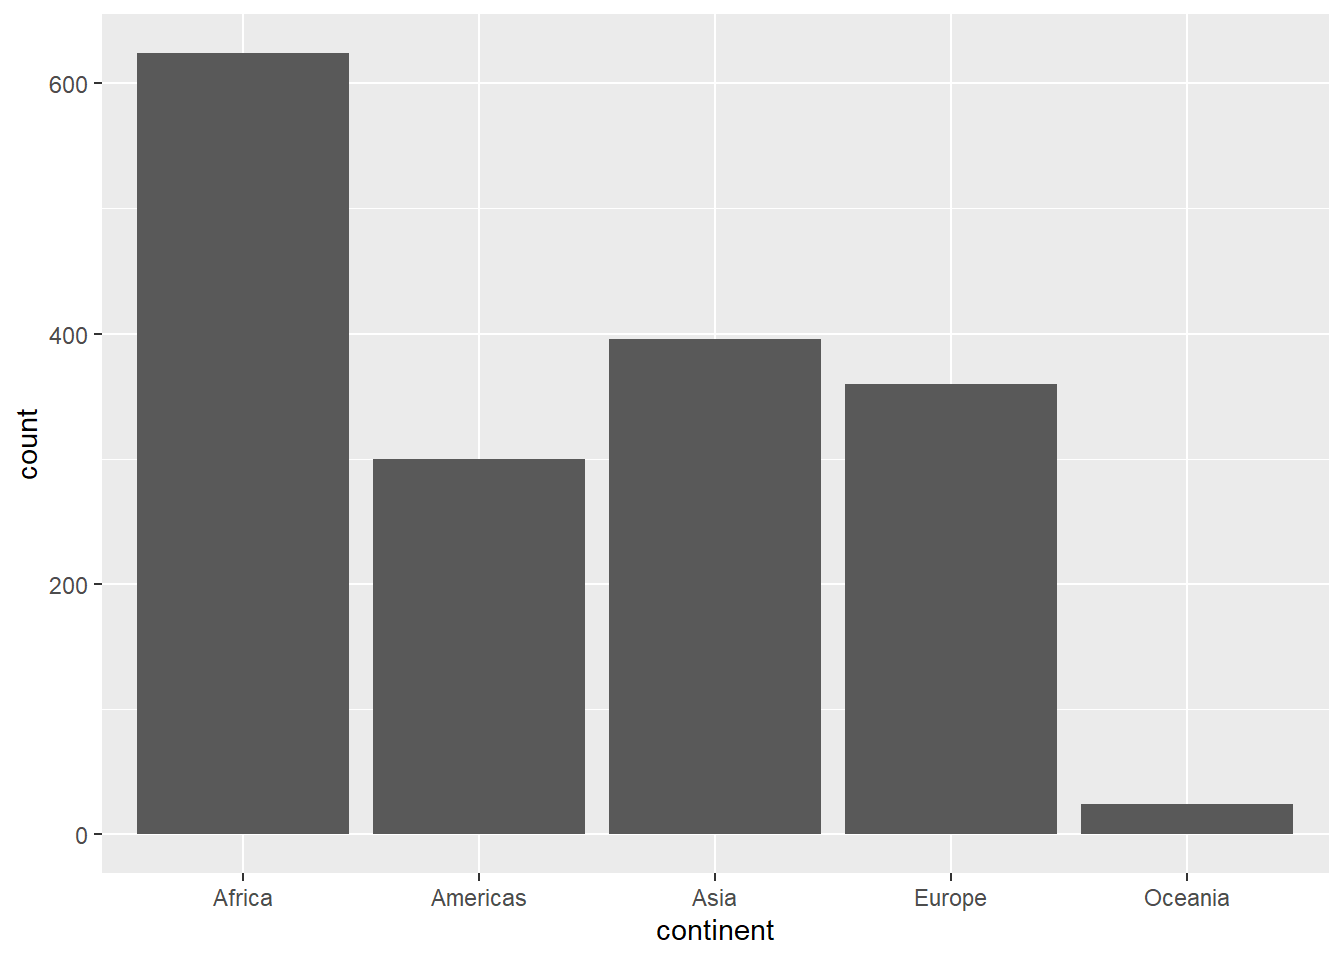
\includegraphics{Applied-Spatial-Data-Analysis_files/figure-latex/unnamed-chunk-4-1.pdf}

\begin{Shaded}
\begin{Highlighting}[]
\FunctionTok{plot}\NormalTok{(poly2\_sg)}
\end{Highlighting}
\end{Shaded}

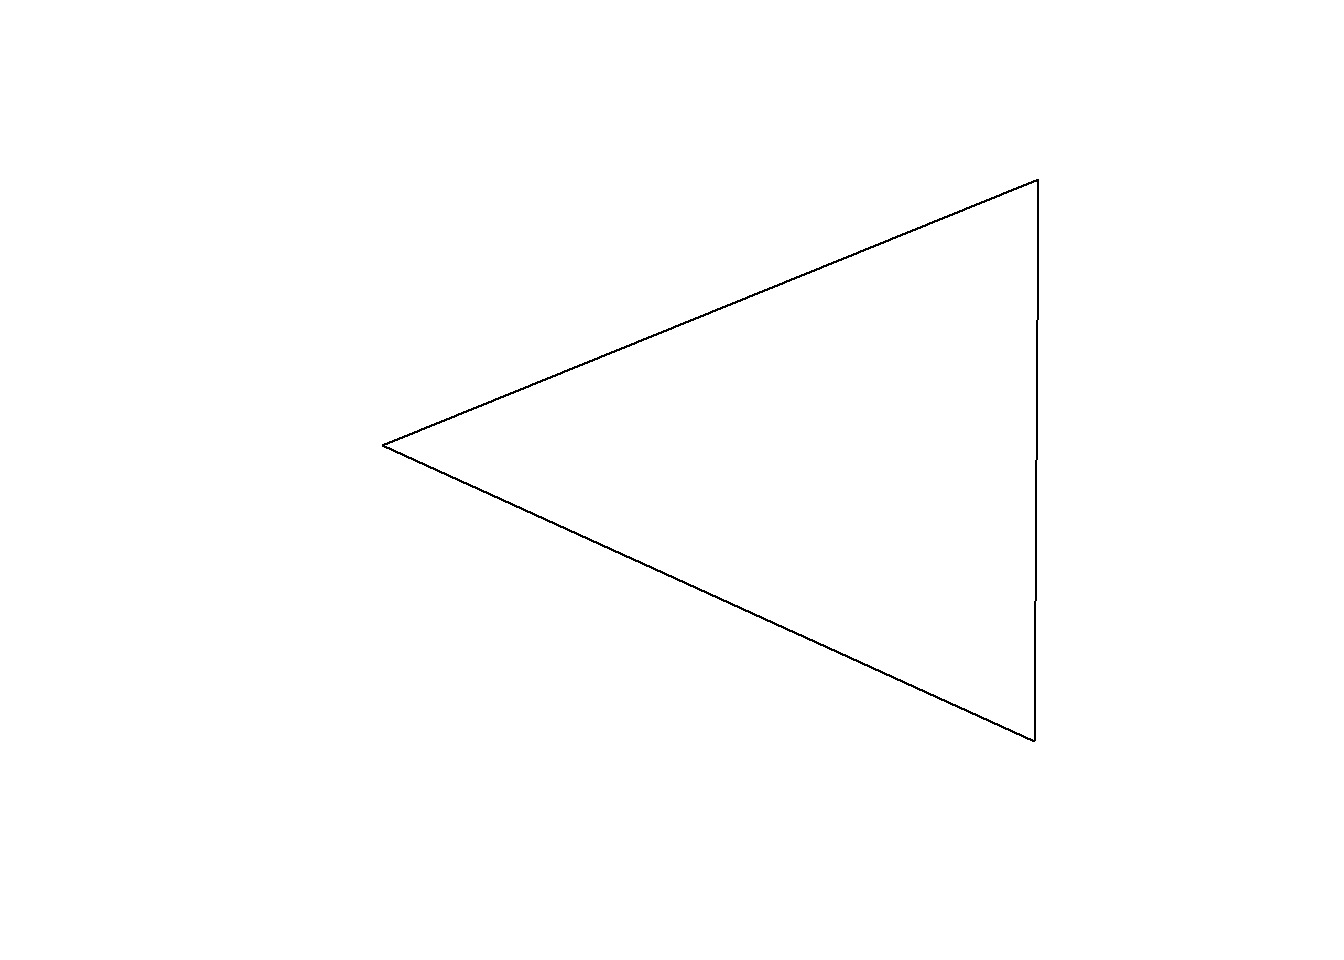
\includegraphics{Applied-Spatial-Data-Analysis_files/figure-latex/unnamed-chunk-4-2.pdf}

\begin{Shaded}
\begin{Highlighting}[]
\CommentTok{\# multipolygon}
\NormalTok{polygons }\OtherTok{\textless{}{-}} \FunctionTok{list}\NormalTok{(poly1, poly2)}
\NormalTok{polygons\_sg }\OtherTok{\textless{}{-}}\NormalTok{ polygons }\SpecialCharTok{\%\textgreater{}\%} \FunctionTok{st\_multipolygon}\NormalTok{()}

\FunctionTok{st\_crs}\NormalTok{(polygons\_sg) }\CommentTok{\# we see that the sf geometry has no CRS set up.}
\end{Highlighting}
\end{Shaded}

\begin{verbatim}
## Coordinate Reference System: NA
\end{verbatim}

\hypertarget{sfc}{%
\subsubsection{sfc}\label{sfc}}

\begin{itemize}
\tightlist
\item
  We usually work with multiple simple features and want to combine them. We have a multipolygon and points and want to combine these. We will use \texttt{st\_sfc()} to merge
\end{itemize}

\begin{Shaded}
\begin{Highlighting}[]
\NormalTok{points\_sfc }\OtherTok{\textless{}{-}} \FunctionTok{st\_sfc}\NormalTok{(point1\_sg, point2\_sg)                   }\CommentTok{\# with no CRS}
\FunctionTok{st\_crs}\NormalTok{(points\_sfc)}
\end{Highlighting}
\end{Shaded}

\begin{verbatim}
## Coordinate Reference System: NA
\end{verbatim}

\begin{Shaded}
\begin{Highlighting}[]
\NormalTok{points\_sfc }\OtherTok{\textless{}{-}} \FunctionTok{st\_sfc}\NormalTok{(point1\_sg, point2\_sg, }\AttributeTok{crs =} \DecValTok{4326}\NormalTok{)       }\CommentTok{\# with appropriate CRS}
\FunctionTok{st\_crs}\NormalTok{(points\_sfc)}
\end{Highlighting}
\end{Shaded}

\begin{verbatim}
## Coordinate Reference System:
##   User input: EPSG:4326 
##   wkt:
## GEOGCRS["WGS 84",
##     DATUM["World Geodetic System 1984",
##         ELLIPSOID["WGS 84",6378137,298.257223563,
##             LENGTHUNIT["metre",1]]],
##     PRIMEM["Greenwich",0,
##         ANGLEUNIT["degree",0.0174532925199433]],
##     CS[ellipsoidal,2],
##         AXIS["geodetic latitude (Lat)",north,
##             ORDER[1],
##             ANGLEUNIT["degree",0.0174532925199433]],
##         AXIS["geodetic longitude (Lon)",east,
##             ORDER[2],
##             ANGLEUNIT["degree",0.0174532925199433]],
##     USAGE[
##         SCOPE["Horizontal component of 3D system."],
##         AREA["World."],
##         BBOX[-90,-180,90,180]],
##     ID["EPSG",4326]]
\end{verbatim}

\begin{Shaded}
\begin{Highlighting}[]
\NormalTok{multipolygon\_sfc }\OtherTok{\textless{}{-}} \FunctionTok{st\_sfc}\NormalTok{(poly1\_sg, poly2\_sg, }\AttributeTok{crs =} \DecValTok{4326}\NormalTok{)}
\FunctionTok{st\_crs}\NormalTok{(multipolygon\_sfc)}
\end{Highlighting}
\end{Shaded}

\begin{verbatim}
## Coordinate Reference System:
##   User input: EPSG:4326 
##   wkt:
## GEOGCRS["WGS 84",
##     DATUM["World Geodetic System 1984",
##         ELLIPSOID["WGS 84",6378137,298.257223563,
##             LENGTHUNIT["metre",1]]],
##     PRIMEM["Greenwich",0,
##         ANGLEUNIT["degree",0.0174532925199433]],
##     CS[ellipsoidal,2],
##         AXIS["geodetic latitude (Lat)",north,
##             ORDER[1],
##             ANGLEUNIT["degree",0.0174532925199433]],
##         AXIS["geodetic longitude (Lon)",east,
##             ORDER[2],
##             ANGLEUNIT["degree",0.0174532925199433]],
##     USAGE[
##         SCOPE["Horizontal component of 3D system."],
##         AREA["World."],
##         BBOX[-90,-180,90,180]],
##     ID["EPSG",4326]]
\end{verbatim}

\hypertarget{sf}{%
\subsubsection{sf}\label{sf}}

We usually have a data frame that stores the attributes of points, polygons, lines. Remember the earthquake magnitude, time, depth for the points; elevation, population, size for the polygons.

For \texttt{point}s

\begin{Shaded}
\begin{Highlighting}[]
\NormalTok{magnitude }\OtherTok{=} \FunctionTok{c}\NormalTok{(}\FloatTok{2.8}\NormalTok{, }\FloatTok{2.7}\NormalTok{)}
\NormalTok{depth }\OtherTok{=} \FunctionTok{c}\NormalTok{(}\FloatTok{8.3}\NormalTok{, }\FloatTok{8.4}\NormalTok{)}
\NormalTok{time }\OtherTok{=} \FunctionTok{c}\NormalTok{(}\DecValTok{1446}\NormalTok{, }\DecValTok{1443}\NormalTok{)}

\NormalTok{earthquake\_marks }\OtherTok{=} \FunctionTok{data.frame}\NormalTok{(magnitude, depth, time)}

\NormalTok{earthquake\_sf }\OtherTok{\textless{}{-}}\NormalTok{ earthquake\_marks }\SpecialCharTok{\%\textgreater{}\%} \FunctionTok{st\_sf}\NormalTok{(}\AttributeTok{geometry =}\NormalTok{ points\_sfc)    }\CommentTok{\# sf object}

\NormalTok{plot1 }\OtherTok{=} \FunctionTok{ggplot}\NormalTok{() }\SpecialCharTok{+} 
  \FunctionTok{geom\_sf}\NormalTok{(}\AttributeTok{data =}\NormalTok{ earthquake\_sf[}\StringTok{"magnitude"}\NormalTok{], }\AttributeTok{color =} \StringTok{"black"}\NormalTok{) }\SpecialCharTok{+}
  \FunctionTok{coord\_sf}\NormalTok{() }
\NormalTok{plot1}
\end{Highlighting}
\end{Shaded}

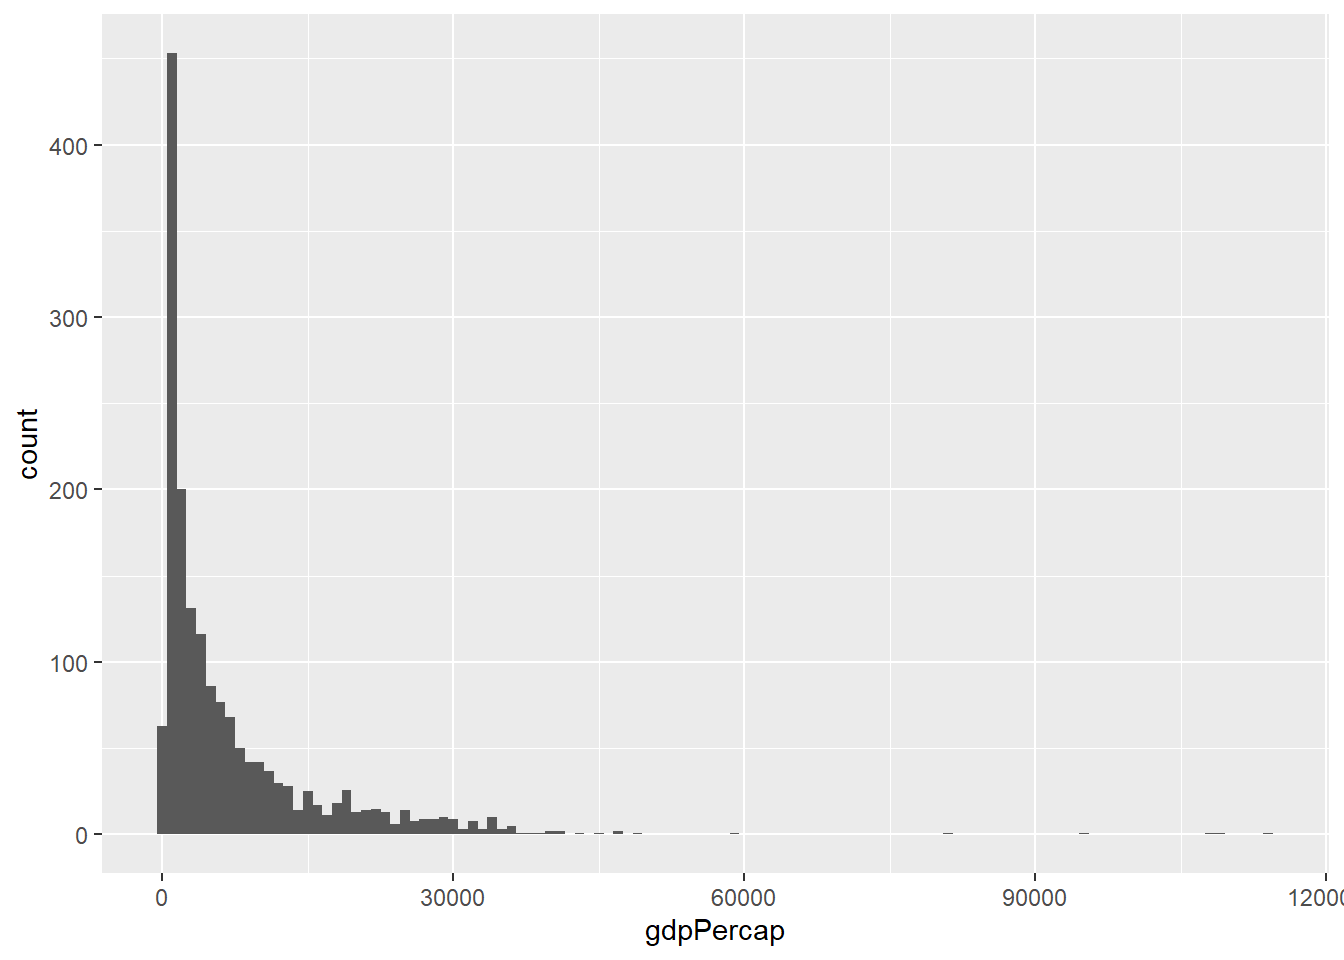
\includegraphics{Applied-Spatial-Data-Analysis_files/figure-latex/unnamed-chunk-6-1.pdf}

\hypertarget{external-files-csv-shp-etc}{%
\subsection{External files (csv, shp etc)}\label{external-files-csv-shp-etc}}

We will use two layers:

\begin{itemize}
\tightlist
\item
  Location of earthquakes - earthquakes
\item
  Boundaries of Turkey as a polygon - turkeyshp
\end{itemize}

One of the files is a shp file, the other one is just a simple csv file.

\begin{itemize}
\tightlist
\item
  Location of earthquakes - earthquakes (from a csv)
\end{itemize}

Read in the dataset as usual

\begin{Shaded}
\begin{Highlighting}[]
\NormalTok{earthquake\_csv }\OtherTok{\textless{}{-}} \FunctionTok{read.csv}\NormalTok{(}\StringTok{"C:/Users/01438475/OneDrive {-} University of Cape Town/ASDA/DataSets/EarthquakesTR.csv"}\NormalTok{)}
\FunctionTok{head}\NormalTok{(earthquake\_csv)}
\end{Highlighting}
\end{Shaded}

\begin{verbatim}
##        Tarih     Saat     Lat    Long Derinlik_km  MD  ML  Mw
## 1 2023.02.07 13:44:51 38.2452 37.9093        13.9 -.- 3.5 -.-
## 2 2023.02.07 13:41:44 38.1057 36.5072         5.0 -.- 3.9 -.-
## 3 2023.02.07 13:37:24 36.4372 35.6998        13.4 -.- 4.0 -.-
## 4 2023.02.07 13:32:27 37.2445 36.9277         5.4 -.- 2.5 -.-
## 5 2023.02.07 13:30:10 38.1428 37.8203         2.0 -.- 2.9 -.-
## 6 2023.02.07 13:27:30 38.3478 38.1357         6.5 -.- 4.7 -.-
##                                Yer
## 1           OREN-AKCADAG (MALATYA)
## 2 MAHMUTBEY-GOKSUN (KAHRAMANMARAS)
## 3     ISKENDERUN KORFEZI (AKDENIZ)
## 4      NAIMLER-NURDAGI (GAZIANTEP)
## 5   FINDIKKOY-DOGANSEHIR (MALATYA)
## 6     KUSDOGAN-YESILYURT (MALATYA)
\end{verbatim}

\begin{Shaded}
\begin{Highlighting}[]
\NormalTok{earthquake\_sf }\OtherTok{\textless{}{-}}\NormalTok{ earthquake\_csv }\SpecialCharTok{\%\textgreater{}\%} 
  \FunctionTok{st\_as\_sf}\NormalTok{(}\AttributeTok{coords =} \FunctionTok{c}\NormalTok{(}\StringTok{"Long"}\NormalTok{, }\StringTok{"Lat"}\NormalTok{), }\AttributeTok{crs =} \DecValTok{4326}\NormalTok{)  }\SpecialCharTok{\%\textgreater{}\%}      \CommentTok{\# convert to sf file \%\textgreater{}\%}
  \CommentTok{\#Here Long comes first.}
  \FunctionTok{st\_transform}\NormalTok{(}\StringTok{"+proj=utm +zone=37 +datum=WGS84 +units=m +no\_defs"}\NormalTok{)                                        }\CommentTok{\# this could be a different CRS}

\FunctionTok{st\_crs}\NormalTok{(earthquake\_sf)}
\end{Highlighting}
\end{Shaded}

\begin{verbatim}
## Coordinate Reference System:
##   User input: +proj=utm +zone=37 +datum=WGS84 +units=m +no_defs 
##   wkt:
## PROJCRS["unknown",
##     BASEGEOGCRS["unknown",
##         DATUM["World Geodetic System 1984",
##             ELLIPSOID["WGS 84",6378137,298.257223563,
##                 LENGTHUNIT["metre",1]],
##             ID["EPSG",6326]],
##         PRIMEM["Greenwich",0,
##             ANGLEUNIT["degree",0.0174532925199433],
##             ID["EPSG",8901]]],
##     CONVERSION["UTM zone 37N",
##         METHOD["Transverse Mercator",
##             ID["EPSG",9807]],
##         PARAMETER["Latitude of natural origin",0,
##             ANGLEUNIT["degree",0.0174532925199433],
##             ID["EPSG",8801]],
##         PARAMETER["Longitude of natural origin",39,
##             ANGLEUNIT["degree",0.0174532925199433],
##             ID["EPSG",8802]],
##         PARAMETER["Scale factor at natural origin",0.9996,
##             SCALEUNIT["unity",1],
##             ID["EPSG",8805]],
##         PARAMETER["False easting",500000,
##             LENGTHUNIT["metre",1],
##             ID["EPSG",8806]],
##         PARAMETER["False northing",0,
##             LENGTHUNIT["metre",1],
##             ID["EPSG",8807]],
##         ID["EPSG",16037]],
##     CS[Cartesian,2],
##         AXIS["(E)",east,
##             ORDER[1],
##             LENGTHUNIT["metre",1,
##                 ID["EPSG",9001]]],
##         AXIS["(N)",north,
##             ORDER[2],
##             LENGTHUNIT["metre",1,
##                 ID["EPSG",9001]]]]
\end{verbatim}

\begin{itemize}
\tightlist
\item
  Boundaries of Turkey as a polygon - turkeyshp
\end{itemize}

\begin{Shaded}
\begin{Highlighting}[]
\FunctionTok{library}\NormalTok{(sf)}
\NormalTok{turkeyshp }\OtherTok{=} \StringTok{"C:/Users/01438475/OneDrive {-} University of Cape Town/ASDA/DataSets/turkey\_administrativelevels0\_1\_2/tur\_polbnda\_adm0.shp"} \SpecialCharTok{\%\textgreater{}\%}
  \FunctionTok{st\_read}\NormalTok{() }\SpecialCharTok{\%\textgreater{}\%}
  \FunctionTok{st\_transform}\NormalTok{(}\StringTok{"+proj=utm +zone=37 +datum=WGS84 +units=m +no\_defs"}\NormalTok{)}
\end{Highlighting}
\end{Shaded}

\begin{verbatim}
## Reading layer `tur_polbnda_adm0' from data source 
##   `C:\Users\01438475\OneDrive - University of Cape Town\ASDA\DataSets\turkey_administrativelevels0_1_2\tur_polbnda_adm0.shp' 
##   using driver `ESRI Shapefile'
## Simple feature collection with 1 feature and 5 fields
## Geometry type: MULTIPOLYGON
## Dimension:     XY
## Bounding box:  xmin: 25.66851 ymin: 35.80842 xmax: 44.81793 ymax: 42.10479
## Geodetic CRS:  WGS 84
\end{verbatim}

Plotting the two together in a simple plot:

\begin{Shaded}
\begin{Highlighting}[]
\FunctionTok{plot}\NormalTok{(}\FunctionTok{st\_geometry}\NormalTok{(turkeyshp))}
\FunctionTok{plot}\NormalTok{(}\FunctionTok{st\_geometry}\NormalTok{(earthquake\_sf), }\AttributeTok{add =} \ConstantTok{TRUE}\NormalTok{, }\AttributeTok{col =} \StringTok{"red"}\NormalTok{)}
\end{Highlighting}
\end{Shaded}

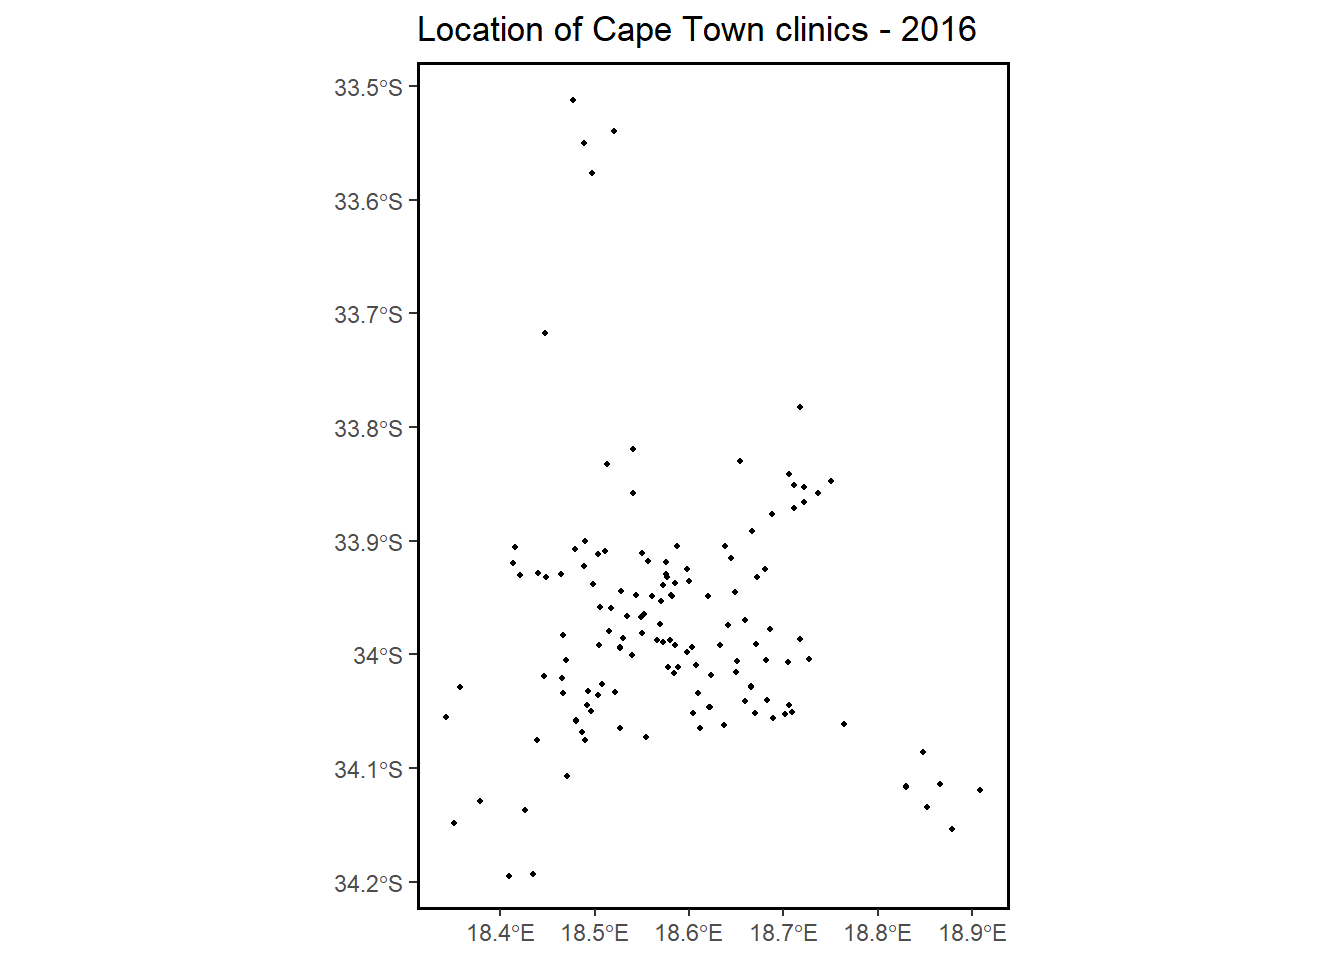
\includegraphics{Applied-Spatial-Data-Analysis_files/figure-latex/unnamed-chunk-9-1.pdf}

or using \texttt{geom\_sf()} in ggplot:

\begin{Shaded}
\begin{Highlighting}[]
\NormalTok{plot1 }\OtherTok{=} \FunctionTok{ggplot}\NormalTok{() }\SpecialCharTok{+}
  \FunctionTok{geom\_sf}\NormalTok{(}\AttributeTok{data =}\NormalTok{ turkeyshp) }\SpecialCharTok{+}
  \FunctionTok{geom\_sf}\NormalTok{(}\AttributeTok{data =}\NormalTok{ earthquake\_sf) }\SpecialCharTok{+}
  \FunctionTok{theme\_minimal}\NormalTok{()}
\end{Highlighting}
\end{Shaded}

Here you see that earthquakes outside of Turkey are also plotted. We can subset only the earthquakes that happened in Turkey:

\begin{Shaded}
\begin{Highlighting}[]
\NormalTok{earthquake\_sf }\OtherTok{=}\NormalTok{ earthquake\_sf[turkeyshp,]}
\NormalTok{plot2 }\OtherTok{=} \FunctionTok{ggplot}\NormalTok{() }\SpecialCharTok{+}
  \FunctionTok{geom\_sf}\NormalTok{(}\AttributeTok{data =}\NormalTok{ turkeyshp) }\SpecialCharTok{+}
  \FunctionTok{geom\_sf}\NormalTok{(}\AttributeTok{data =}\NormalTok{ earthquake\_sf) }\SpecialCharTok{+}
  \FunctionTok{theme\_minimal}\NormalTok{()}
\end{Highlighting}
\end{Shaded}

Visualisations can be done via \texttt{tmap} package as well, and can be saved as png, html files.

\begin{Shaded}
\begin{Highlighting}[]
\FunctionTok{tmap\_mode}\NormalTok{(}\StringTok{"view"}\NormalTok{)}
\end{Highlighting}
\end{Shaded}

\begin{verbatim}
## tmap mode set to interactive viewing
\end{verbatim}

\begin{Shaded}
\begin{Highlighting}[]
\NormalTok{tmap1 }\OtherTok{=} \FunctionTok{tm\_shape}\NormalTok{(turkeyshp)}\SpecialCharTok{+}\FunctionTok{tm\_polygons}\NormalTok{() }\SpecialCharTok{+}\FunctionTok{tm\_shape}\NormalTok{(earthquake\_sf) }\SpecialCharTok{+} \FunctionTok{tm\_dots}\NormalTok{()}
\FunctionTok{tmap\_save}\NormalTok{(tmap1, }\AttributeTok{filename=} \StringTok{"turkeyearthquakes.html"}\NormalTok{)}
\end{Highlighting}
\end{Shaded}

\begin{verbatim}
## Interactive map saved to C:\Users\01438475\OneDrive - University of Cape Town\ASDA\bookdown-demo-master\turkeyearthquakes.html
\end{verbatim}

\hypertarget{simulated-datasets}{%
\subsection{Simulated Datasets}\label{simulated-datasets}}

\hypertarget{csr-data-points}{%
\paragraph{CSR Data Points}\label{csr-data-points}}

\begin{Shaded}
\begin{Highlighting}[]
\FunctionTok{set.seed}\NormalTok{(}\DecValTok{135}\NormalTok{)}
\NormalTok{xy\_csr }\OtherTok{\textless{}{-}} \FunctionTok{matrix}\NormalTok{(}\FunctionTok{runif}\NormalTok{(}\DecValTok{80}\NormalTok{), }\AttributeTok{ncol=}\DecValTok{2}\NormalTok{)}
\NormalTok{pp\_csr }\OtherTok{\textless{}{-}} \FunctionTok{as.ppp}\NormalTok{(xy\_csr, }\FunctionTok{c}\NormalTok{(}\DecValTok{0}\NormalTok{,}\DecValTok{1}\NormalTok{,}\DecValTok{0}\NormalTok{,}\DecValTok{1}\NormalTok{))}
\FunctionTok{plot}\NormalTok{(pp\_csr)}
\end{Highlighting}
\end{Shaded}

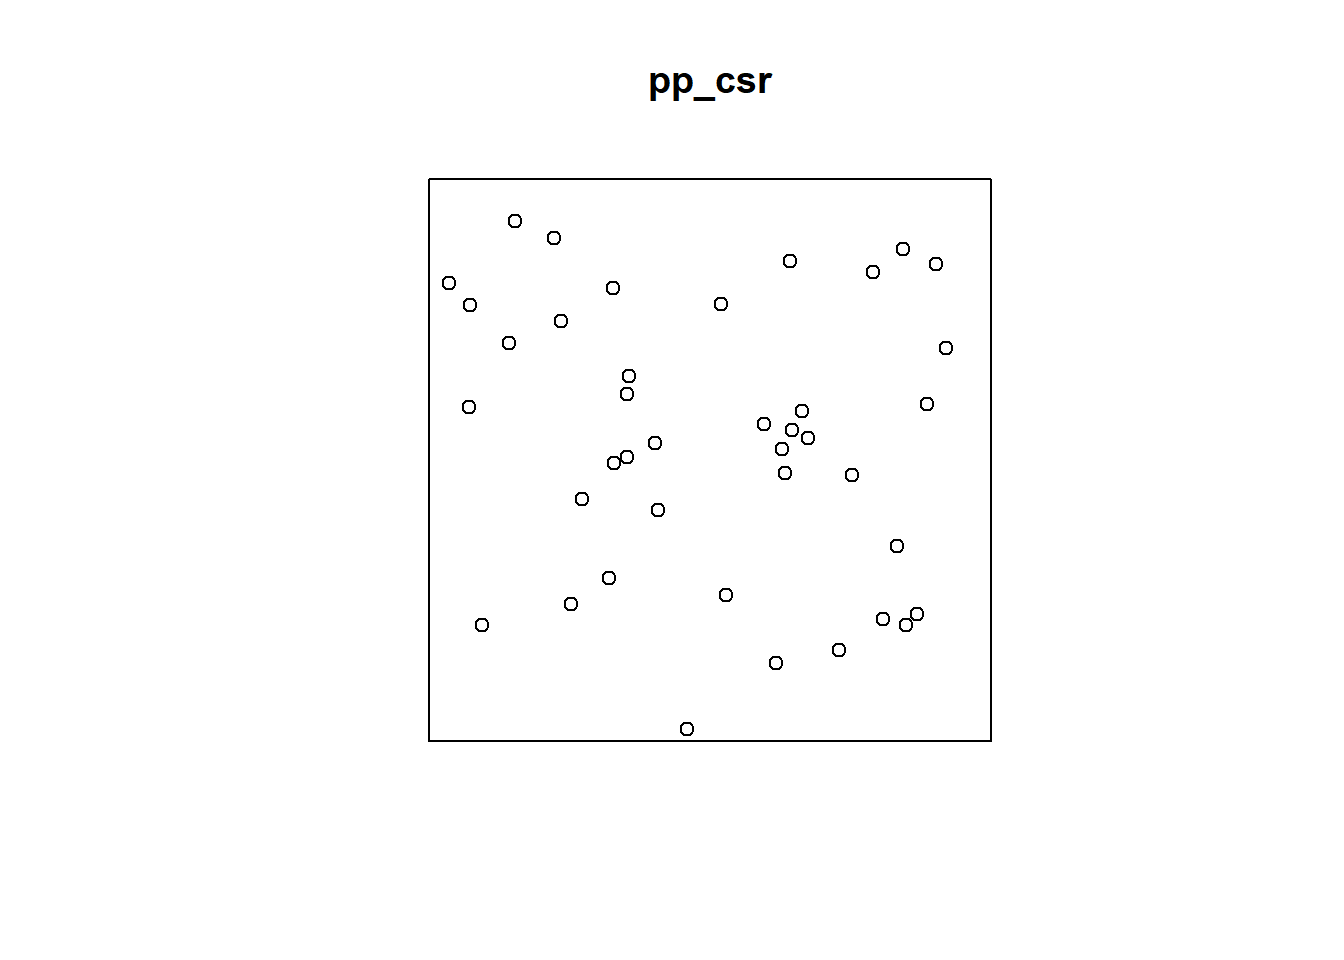
\includegraphics{Applied-Spatial-Data-Analysis_files/figure-latex/xy_csr-1.pdf}

\hypertarget{csr-data-points-with-marks}{%
\paragraph{CSR Data Points with Marks}\label{csr-data-points-with-marks}}

\begin{Shaded}
\begin{Highlighting}[]
\FunctionTok{set.seed}\NormalTok{(}\DecValTok{135}\NormalTok{)}
\NormalTok{xy\_csr }\OtherTok{\textless{}{-}} \FunctionTok{matrix}\NormalTok{(}\FunctionTok{runif}\NormalTok{(}\DecValTok{2000}\NormalTok{), }\AttributeTok{ncol=}\DecValTok{2}\NormalTok{)}
\NormalTok{mark\_numerical }\OtherTok{=} \FunctionTok{rexp}\NormalTok{(}\DecValTok{1000}\NormalTok{)}
\NormalTok{mark\_categorical }\OtherTok{=}  \FunctionTok{sample}\NormalTok{(}\DecValTok{0}\SpecialCharTok{:}\DecValTok{1}\NormalTok{,}\AttributeTok{size=}\DecValTok{1000}\NormalTok{,}\AttributeTok{replace=}\ConstantTok{TRUE}\NormalTok{)}

\CommentTok{\# plot without marks}
\NormalTok{pp\_csr\_m }\OtherTok{\textless{}{-}} \FunctionTok{as.ppp}\NormalTok{(xy\_csr, }\FunctionTok{c}\NormalTok{(}\DecValTok{0}\NormalTok{,}\DecValTok{1}\NormalTok{,}\DecValTok{0}\NormalTok{,}\DecValTok{1}\NormalTok{))}
\FunctionTok{plot}\NormalTok{(pp\_csr\_m)}
\end{Highlighting}
\end{Shaded}

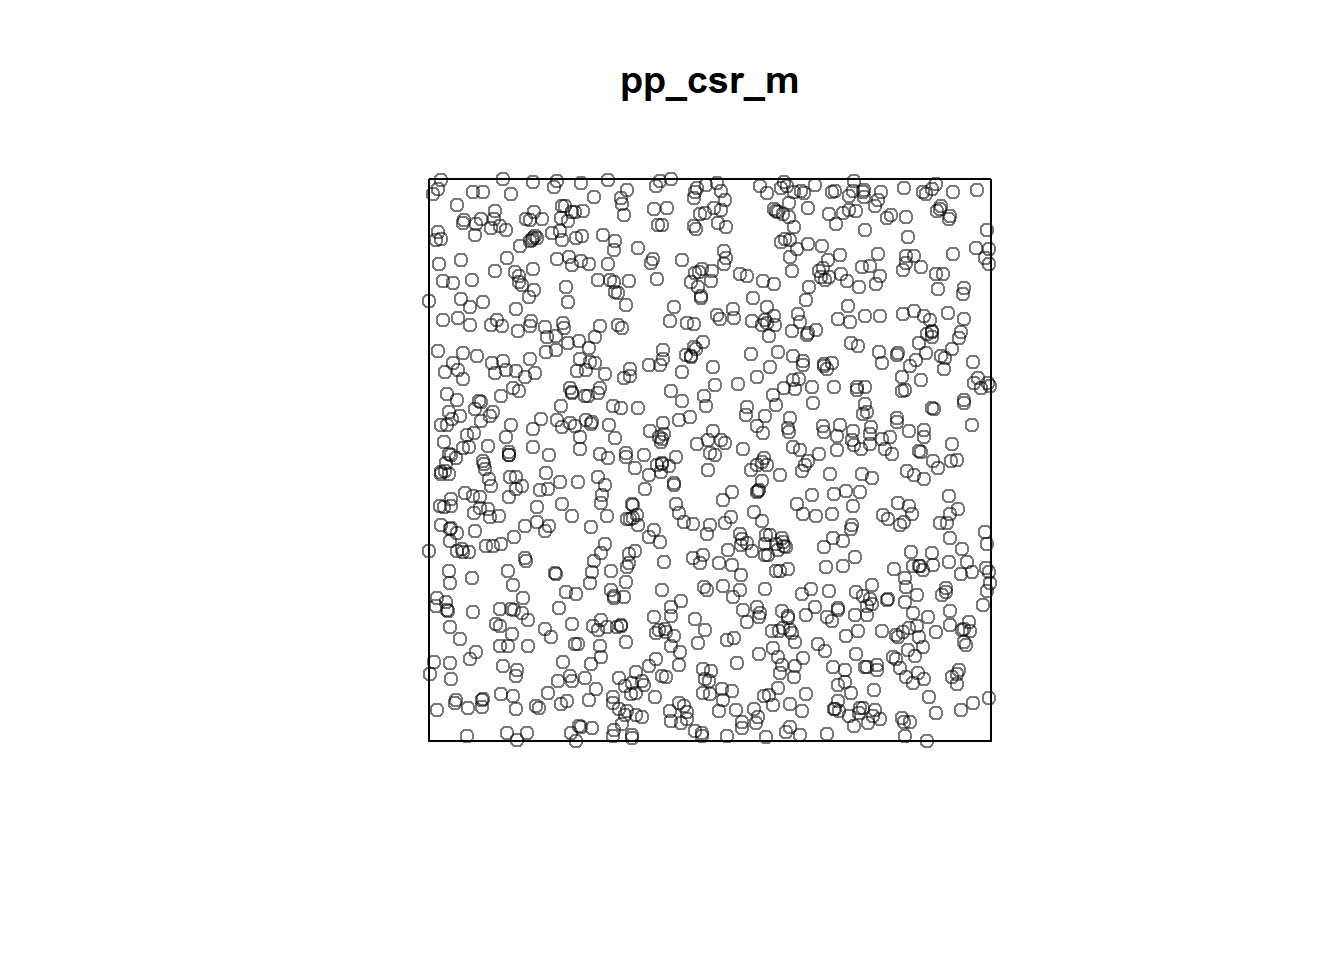
\includegraphics{Applied-Spatial-Data-Analysis_files/figure-latex/xy_csr with marks-1.pdf}

\begin{Shaded}
\begin{Highlighting}[]
\CommentTok{\# plot with marks}
\NormalTok{xy\_csr\_withmark }\OtherTok{=} \FunctionTok{as.data.frame}\NormalTok{(}\FunctionTok{cbind}\NormalTok{(xy\_csr,mark\_numerical, mark\_categorical))}

\CommentTok{\# The categorical variable needs to be set as factor with clearly defined levels}

\NormalTok{xy\_csr\_withmark}\SpecialCharTok{$}\NormalTok{mark\_categorical }\OtherTok{=} \FunctionTok{factor}\NormalTok{(xy\_csr\_withmark}\SpecialCharTok{$}\NormalTok{mark\_categorical, }\AttributeTok{levels =} \FunctionTok{c}\NormalTok{(}\StringTok{"0"}\NormalTok{,}\StringTok{"1"}\NormalTok{))}

\CommentTok{\# set as point pattern}

\NormalTok{pp\_csr\_withmark }\OtherTok{=} \FunctionTok{with}\NormalTok{(xy\_csr\_withmark, }\FunctionTok{ppp}\NormalTok{(V1,V2,}\FunctionTok{c}\NormalTok{(}\DecValTok{0}\NormalTok{,}\DecValTok{1}\NormalTok{),}\FunctionTok{c}\NormalTok{(}\DecValTok{0}\NormalTok{,}\DecValTok{1}\NormalTok{),}\AttributeTok{marks=}\NormalTok{xy\_csr\_withmark[,}\DecValTok{4}\NormalTok{]))}
\FunctionTok{plot}\NormalTok{(pp\_csr\_withmark)}
\end{Highlighting}
\end{Shaded}

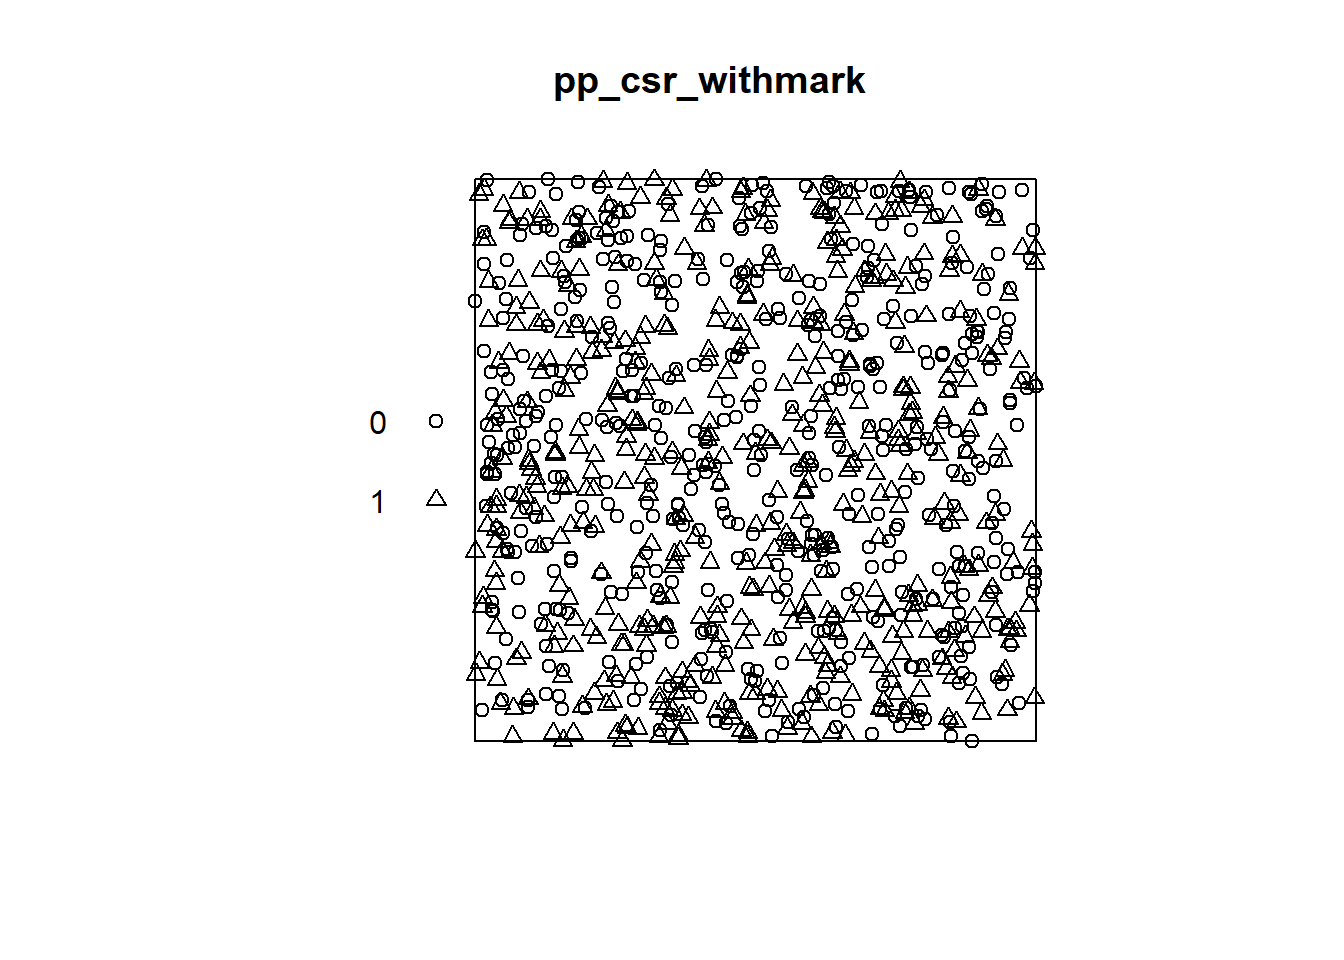
\includegraphics{Applied-Spatial-Data-Analysis_files/figure-latex/xy_csr with marks-2.pdf}

\hypertarget{regular-data-points}{%
\paragraph{Regular Data Points}\label{regular-data-points}}

\begin{Shaded}
\begin{Highlighting}[]
\NormalTok{regular }\OtherTok{\textless{}{-}} \FunctionTok{read.csv}\NormalTok{(}\StringTok{"C:/Users/01438475/OneDrive {-} University of Cape Town/ASDA/regular.csv"}\NormalTok{)}
\NormalTok{xy\_regular }\OtherTok{\textless{}{-}} \FunctionTok{matrix}\NormalTok{(}\FunctionTok{cbind}\NormalTok{(regular}\SpecialCharTok{$}\NormalTok{X,regular}\SpecialCharTok{$}\NormalTok{Y), }\AttributeTok{ncol=}\DecValTok{2}\NormalTok{)}
\NormalTok{pp\_regular }\OtherTok{\textless{}{-}} \FunctionTok{as.ppp}\NormalTok{(xy\_regular, }\FunctionTok{c}\NormalTok{(}\DecValTok{0}\NormalTok{,}\DecValTok{1}\NormalTok{,}\DecValTok{0}\NormalTok{,}\DecValTok{1}\NormalTok{))}
\FunctionTok{plot}\NormalTok{(pp\_regular)}
\end{Highlighting}
\end{Shaded}

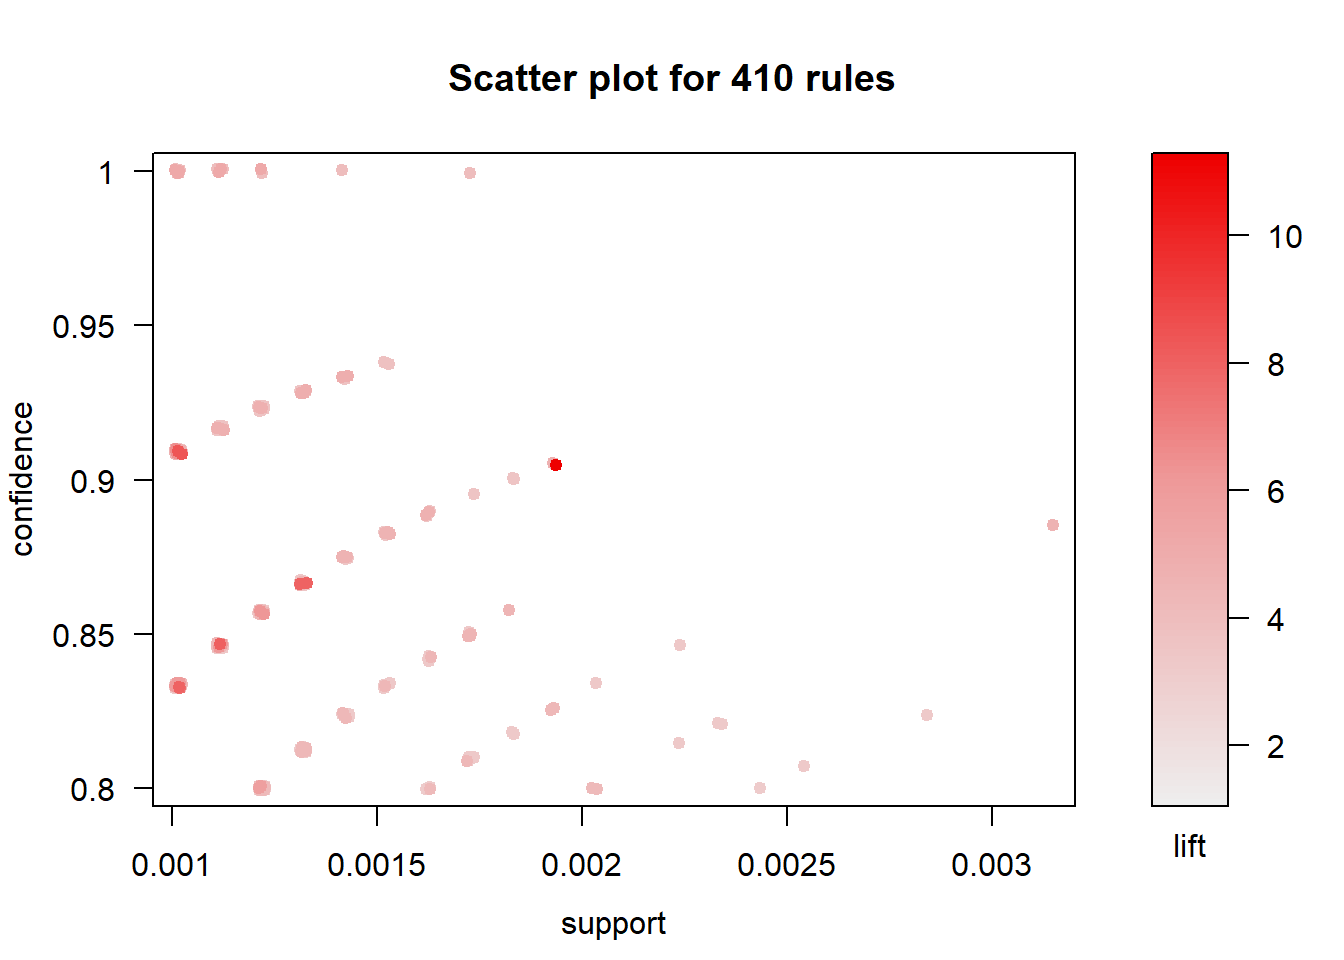
\includegraphics{Applied-Spatial-Data-Analysis_files/figure-latex/unnamed-chunk-13-1.pdf}

\hypertarget{cluster-data-points}{%
\paragraph{Cluster Data Points}\label{cluster-data-points}}

\begin{Shaded}
\begin{Highlighting}[]
\NormalTok{cluster }\OtherTok{\textless{}{-}} \FunctionTok{read.csv}\NormalTok{(}\StringTok{"C:/Users/01438475/OneDrive {-} University of Cape Town/ASDA/cluster.csv"}\NormalTok{)}
\NormalTok{xy\_cluster }\OtherTok{\textless{}{-}} \FunctionTok{matrix}\NormalTok{(}\FunctionTok{cbind}\NormalTok{(cluster}\SpecialCharTok{$}\NormalTok{X,cluster}\SpecialCharTok{$}\NormalTok{Y), }\AttributeTok{ncol=}\DecValTok{2}\NormalTok{)}
\NormalTok{pp\_cluster }\OtherTok{\textless{}{-}} \FunctionTok{as.ppp}\NormalTok{(xy\_cluster, }\FunctionTok{c}\NormalTok{(}\DecValTok{0}\NormalTok{,}\DecValTok{1}\NormalTok{,}\DecValTok{0}\NormalTok{,}\DecValTok{1}\NormalTok{))}
\FunctionTok{plot}\NormalTok{(pp\_cluster)}
\end{Highlighting}
\end{Shaded}

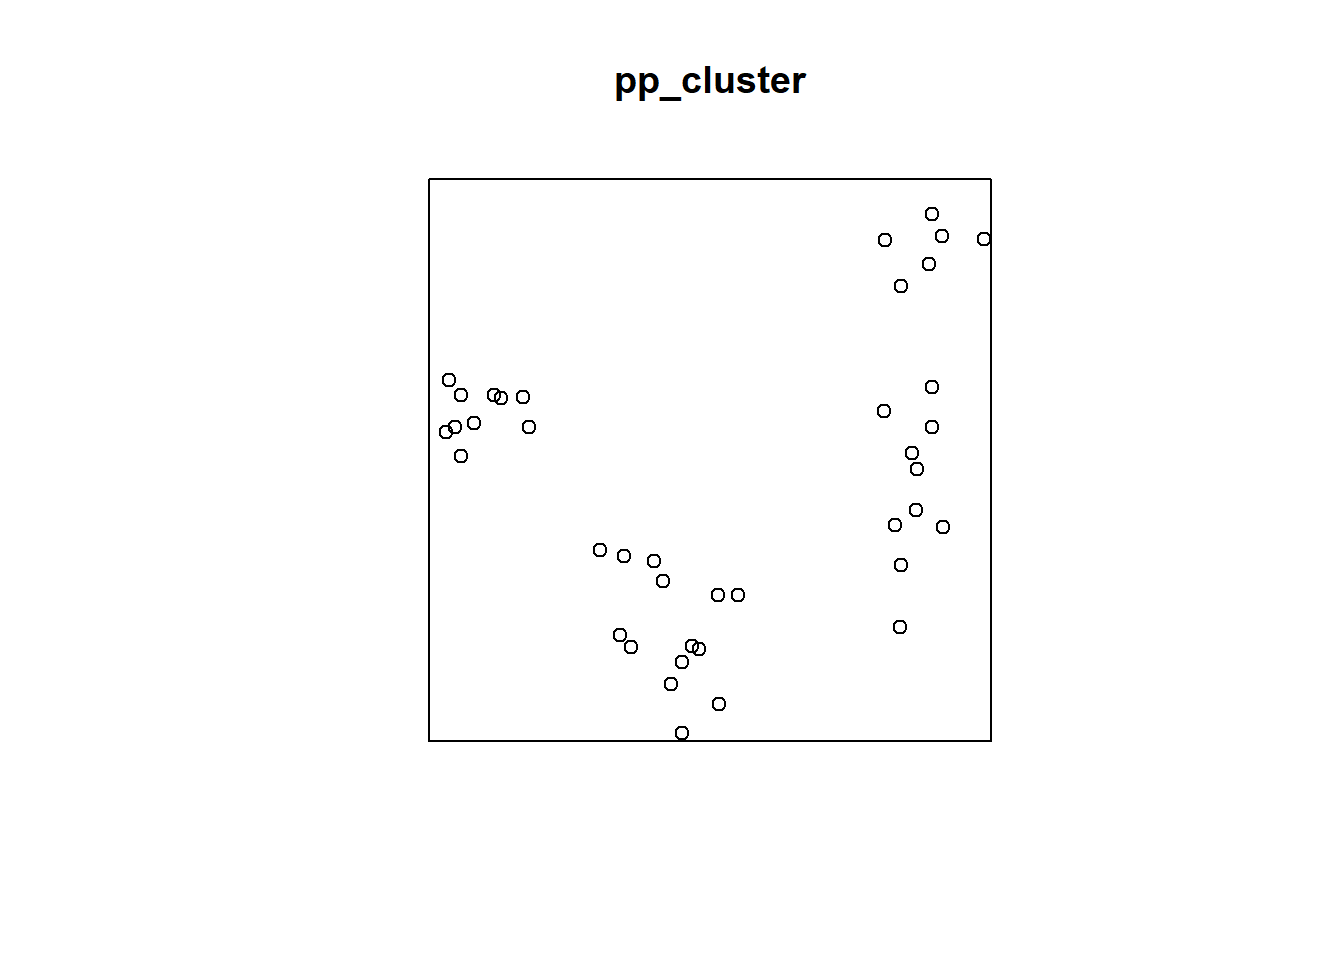
\includegraphics{Applied-Spatial-Data-Analysis_files/figure-latex/unnamed-chunk-14-1.pdf}

\hypertarget{swedishpines-dataset-from-spatstat.data-library}{%
\subsection{Swedishpines Dataset from spatstat.data library}\label{swedishpines-dataset-from-spatstat.data-library}}

\begin{Shaded}
\begin{Highlighting}[]
\FunctionTok{data}\NormalTok{(swedishpines)}
\NormalTok{swp }\OtherTok{=} \FunctionTok{rescale.ppp}\NormalTok{(swedishpines)}
\NormalTok{swp}
\end{Highlighting}
\end{Shaded}

\begin{Shaded}
\begin{Highlighting}[]
\NormalTok{\#\# Planar point pattern: 71 points}
\NormalTok{\#\# window: rectangle = [0, 9.6] x [0, 10] metres}
\end{Highlighting}
\end{Shaded}

\begin{Shaded}
\begin{Highlighting}[]
\FunctionTok{class}\NormalTok{(swp)}
\end{Highlighting}
\end{Shaded}

\begin{Shaded}
\begin{Highlighting}[]
\NormalTok{\#\# [1] "ppp"}
\end{Highlighting}
\end{Shaded}

\begin{Shaded}
\begin{Highlighting}[]
\FunctionTok{summary}\NormalTok{(swp)}
\end{Highlighting}
\end{Shaded}

\begin{Shaded}
\begin{Highlighting}[]
\NormalTok{\#\# Planar point pattern:  71 points}
\NormalTok{\#\# Average intensity 0.7395833 points per square metre}
\NormalTok{\#\# }
\NormalTok{\#\# Coordinates are given to 1 decimal place}
\NormalTok{\#\# i.e. rounded to the nearest multiple of 0.1 metres}
\NormalTok{\#\# }
\NormalTok{\#\# Window: rectangle = [0, 9.6] x [0, 10] metres}
\NormalTok{\#\# Window area = 96 square metres}
\NormalTok{\#\# Unit of length: 1 metre}
\end{Highlighting}
\end{Shaded}

\begin{Shaded}
\begin{Highlighting}[]
\FunctionTok{plot}\NormalTok{(swp)}
\end{Highlighting}
\end{Shaded}

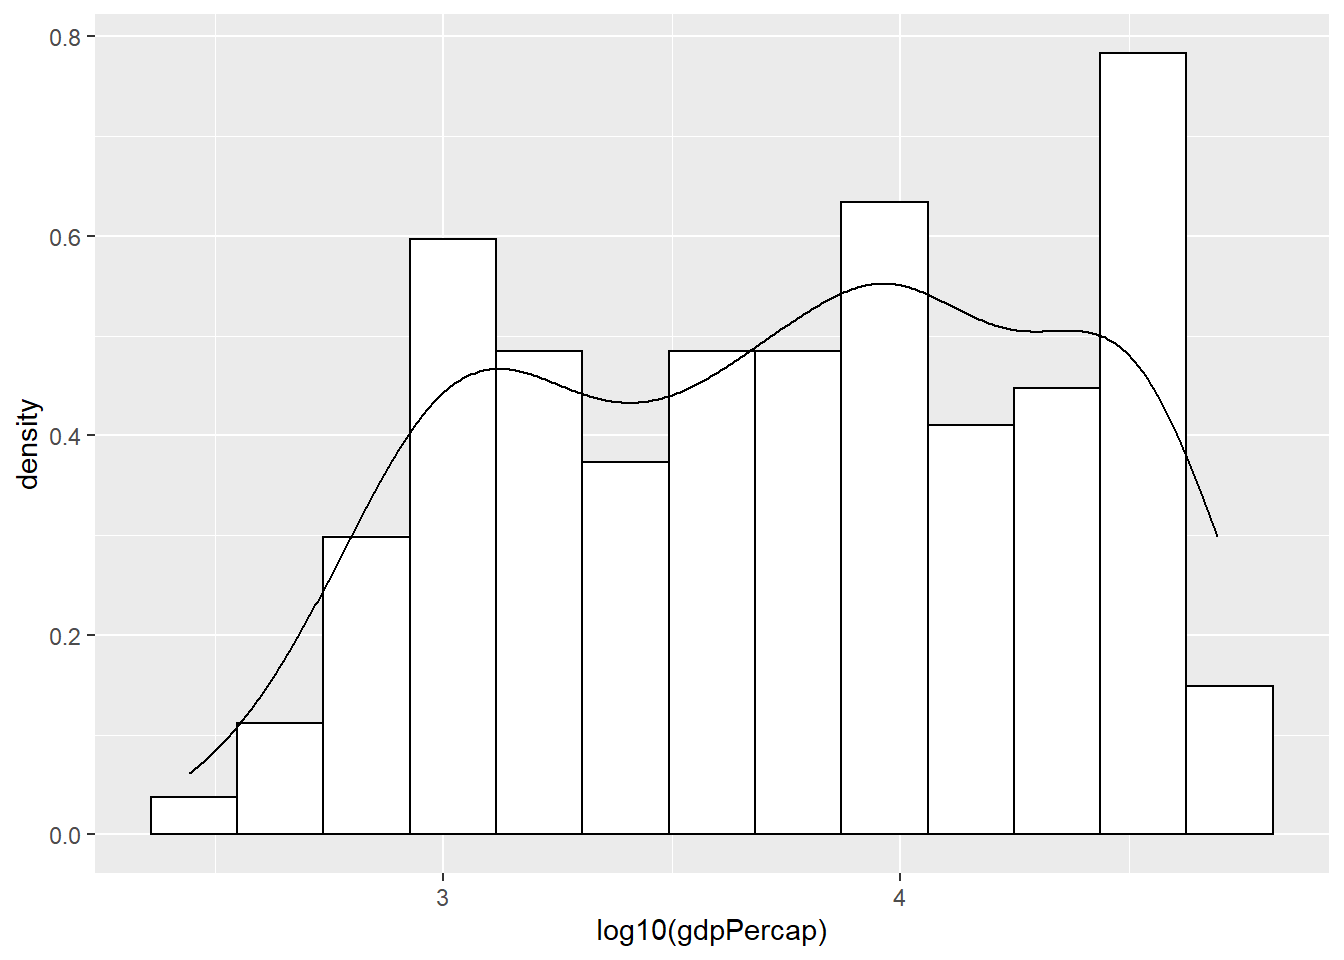
\includegraphics{Applied-Spatial-Data-Analysis_files/figure-latex/unnamed-chunk-15-1.pdf}

\hypertarget{external-datasets---turkey}{%
\subsection{External datasets - Turkey}\label{external-datasets---turkey}}

Let us go back to Earthquake data that we converted to sf object.

Convert the \texttt{sf} objects to \texttt{ppp} point pattern object using function \texttt{as.ppp} so that we can analyse them in R with spatstat.

\begin{Shaded}
\begin{Highlighting}[]
\CommentTok{\# only the geometry}
\NormalTok{earthquake\_ppp }\OtherTok{=} \FunctionTok{as.ppp}\NormalTok{(}\FunctionTok{st\_geometry}\NormalTok{(earthquake\_sf))}
\NormalTok{turkeyshp\_owin }\OtherTok{=} \FunctionTok{as.owin}\NormalTok{(}\FunctionTok{st\_geometry}\NormalTok{(turkeyshp))}

\FunctionTok{plot}\NormalTok{(earthquake\_ppp)}
\end{Highlighting}
\end{Shaded}

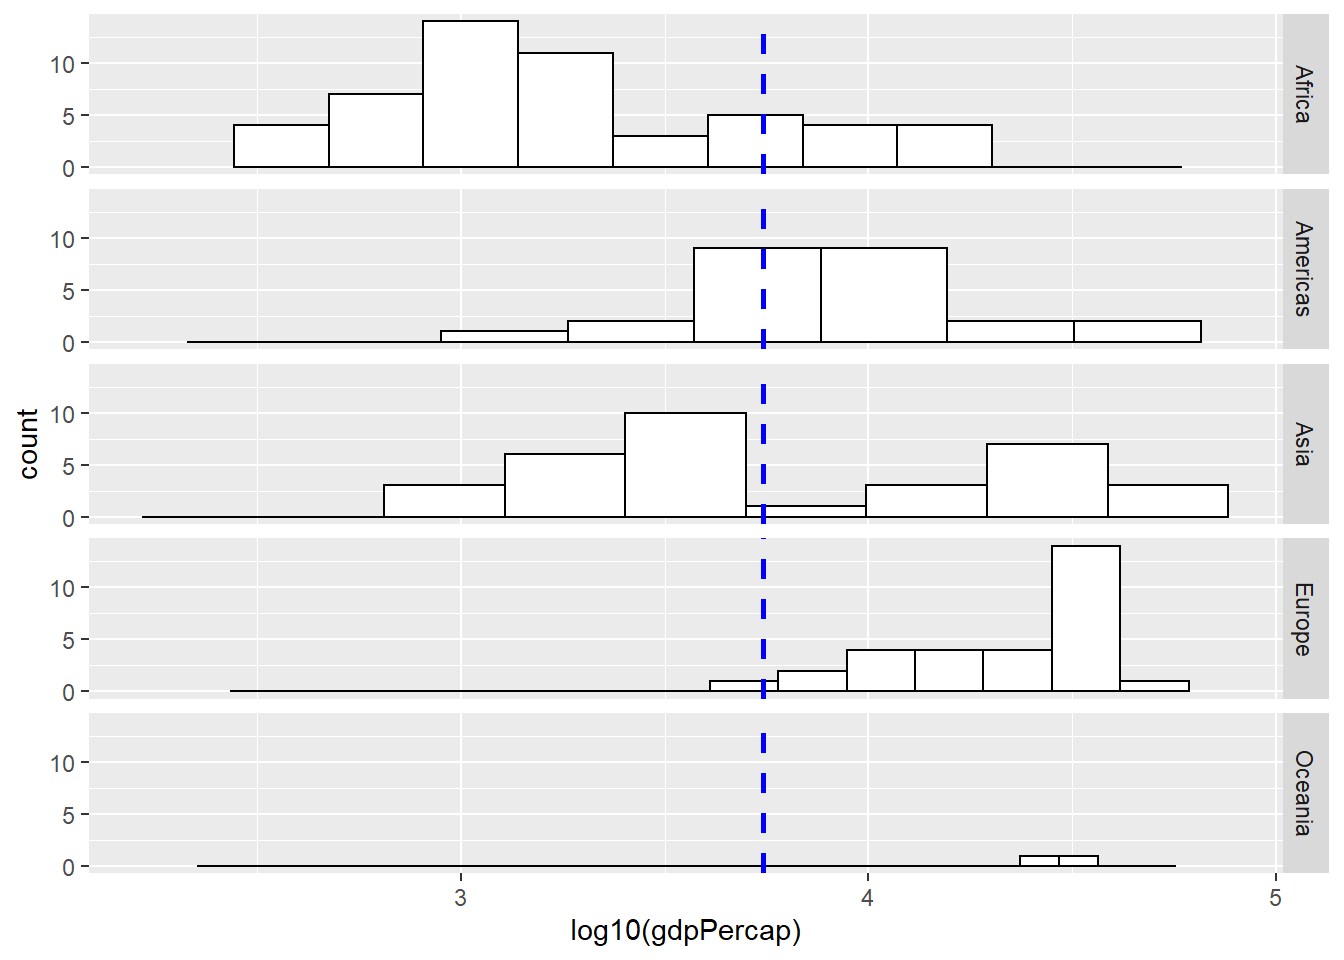
\includegraphics{Applied-Spatial-Data-Analysis_files/figure-latex/unnamed-chunk-16-1.pdf}

\begin{Shaded}
\begin{Highlighting}[]
\FunctionTok{plot}\NormalTok{(turkeyshp\_owin)}
\end{Highlighting}
\end{Shaded}

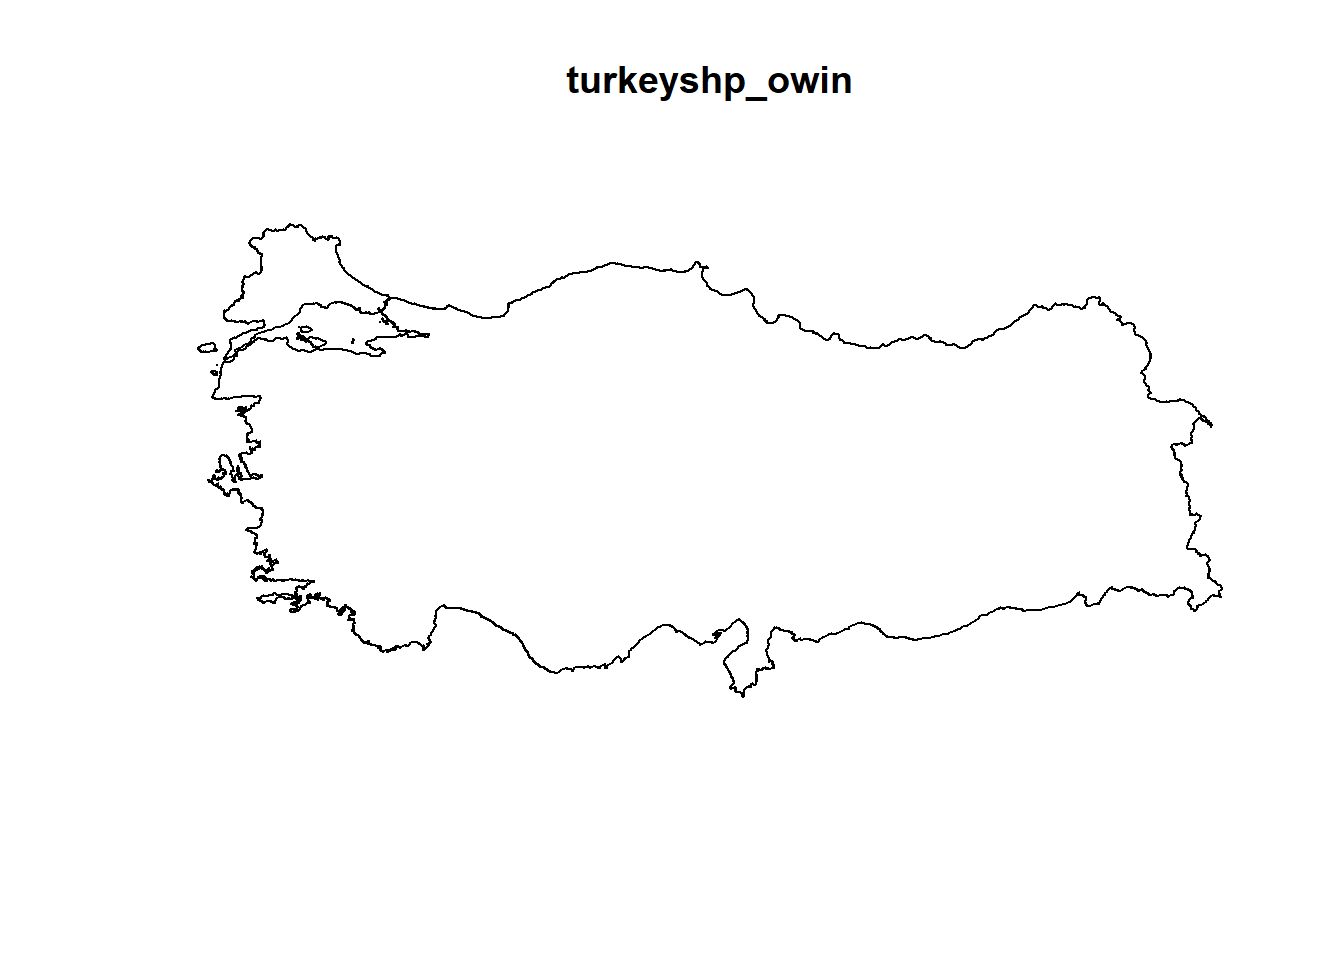
\includegraphics{Applied-Spatial-Data-Analysis_files/figure-latex/unnamed-chunk-16-2.pdf}

The observation window and the point pattern can be combined, so that the custom window replaces the default rectangular window:

\begin{Shaded}
\begin{Highlighting}[]
\NormalTok{earthquake\_ppp }\OtherTok{=}\NormalTok{ earthquake\_ppp[turkeyshp\_owin]}
\FunctionTok{plot}\NormalTok{(earthquake\_ppp)}
\end{Highlighting}
\end{Shaded}

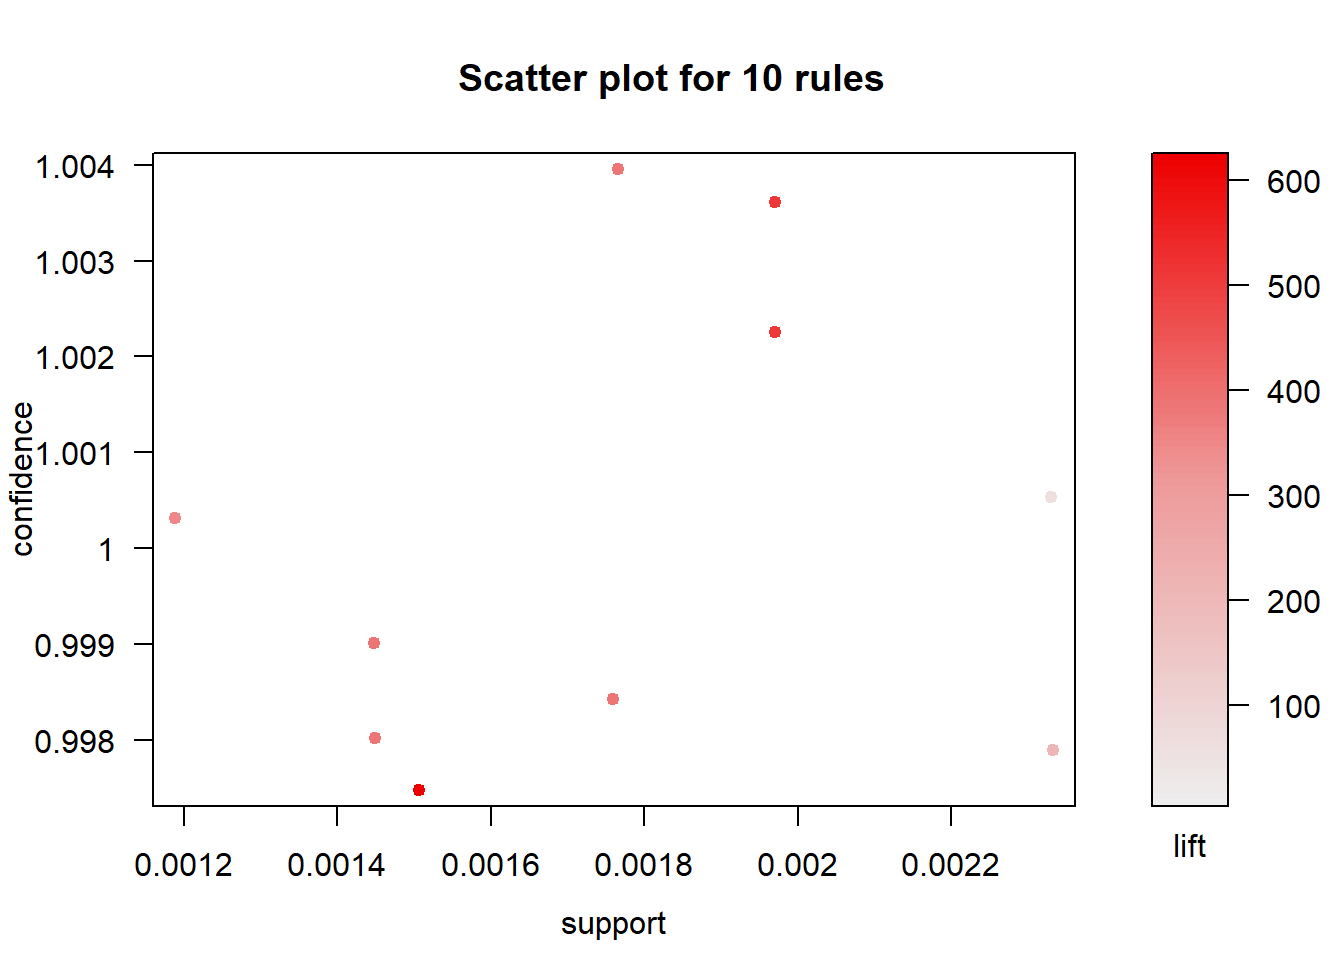
\includegraphics{Applied-Spatial-Data-Analysis_files/figure-latex/unnamed-chunk-17-1.pdf}

We might want to incorporate some marks to these points:

\begin{Shaded}
\begin{Highlighting}[]
\CommentTok{\# if there are marks that need to be included:}

\NormalTok{earthquake\_ppp.marked\_numeric }\OtherTok{\textless{}{-}} \FunctionTok{ppp}\NormalTok{(earthquake\_ppp}\SpecialCharTok{$}\NormalTok{x, earthquake\_ppp}\SpecialCharTok{$}\NormalTok{y, }\AttributeTok{window =}\NormalTok{ turkeyshp\_owin, }\AttributeTok{marks =}\FunctionTok{data.frame}\NormalTok{(earthquake\_sf)}\SpecialCharTok{$}\NormalTok{ML)}

\FunctionTok{plot}\NormalTok{(earthquake\_ppp.marked\_numeric, }\AttributeTok{use.marks=}\ConstantTok{TRUE}\NormalTok{)}
\end{Highlighting}
\end{Shaded}

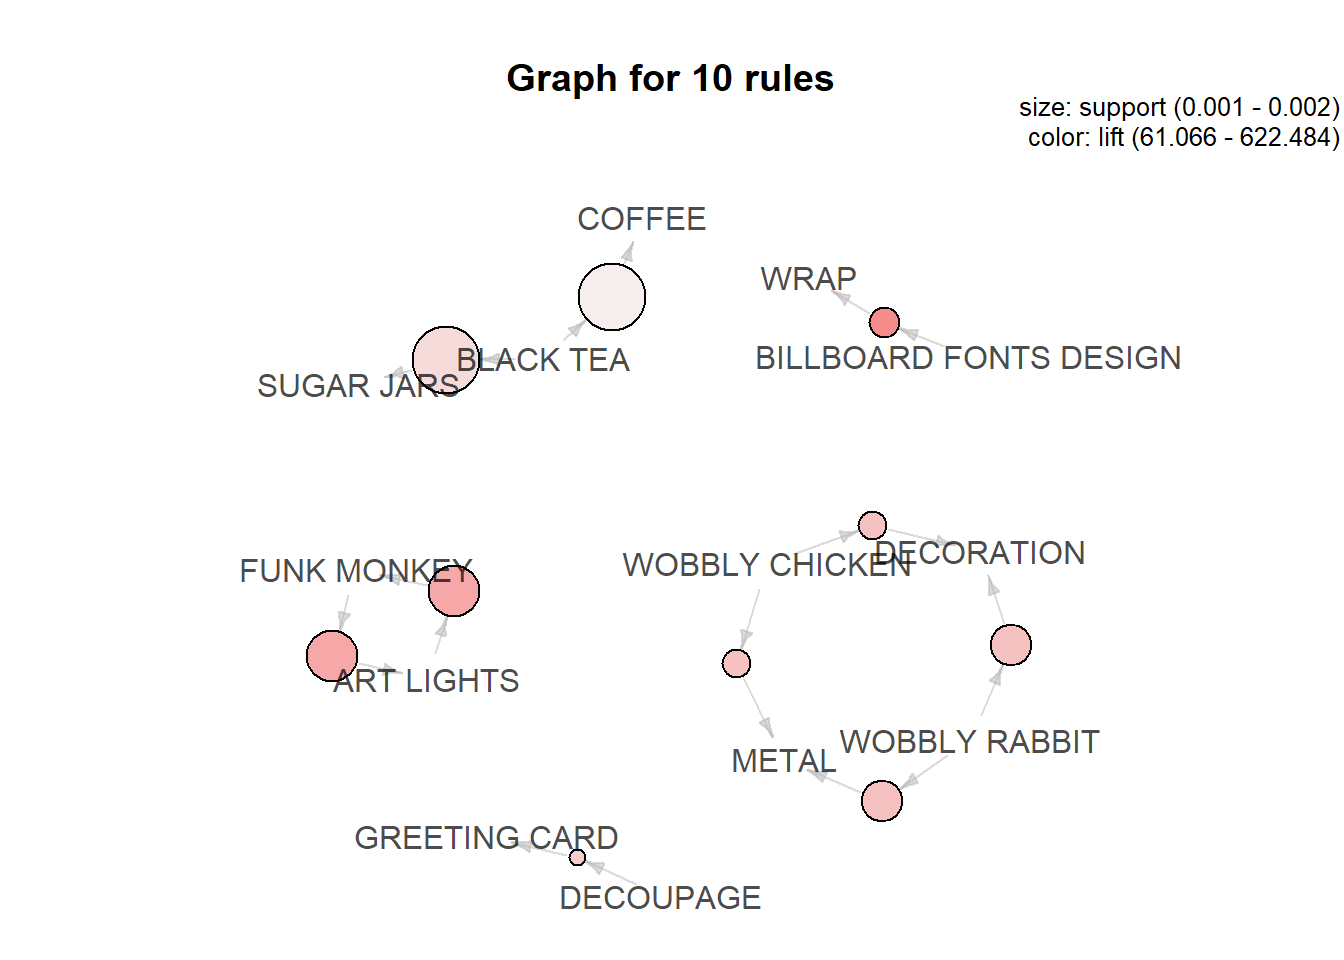
\includegraphics{Applied-Spatial-Data-Analysis_files/figure-latex/unnamed-chunk-18-1.pdf}

\begin{Shaded}
\begin{Highlighting}[]
\NormalTok{earthquake\_ppp.marked\_categorical }\OtherTok{\textless{}{-}} \FunctionTok{ppp}\NormalTok{(earthquake\_ppp}\SpecialCharTok{$}\NormalTok{x, earthquake\_ppp}\SpecialCharTok{$}\NormalTok{y, }\AttributeTok{window =}\NormalTok{ turkeyshp\_owin, }\AttributeTok{marks =}\FunctionTok{ifelse}\NormalTok{(}\FunctionTok{data.frame}\NormalTok{(earthquake\_sf)}\SpecialCharTok{$}\NormalTok{ML}\SpecialCharTok{\textless{}}\DecValTok{5}\NormalTok{,}\StringTok{"low"}\NormalTok{,}\StringTok{"high"}\NormalTok{))}

\FunctionTok{plot}\NormalTok{(earthquake\_ppp.marked\_categorical, }\AttributeTok{use.marks=}\ConstantTok{TRUE}\NormalTok{, }
     \AttributeTok{cols=}\FunctionTok{c}\NormalTok{(}\StringTok{"red"}\NormalTok{,}\StringTok{"blue"}\NormalTok{,}\StringTok{"pink"}\NormalTok{),}
     \AttributeTok{markscale=}\FloatTok{0.1}\NormalTok{,}
     \AttributeTok{pch=}\DecValTok{21}\NormalTok{, }\AttributeTok{cex=}\DecValTok{1}\NormalTok{)}
\end{Highlighting}
\end{Shaded}

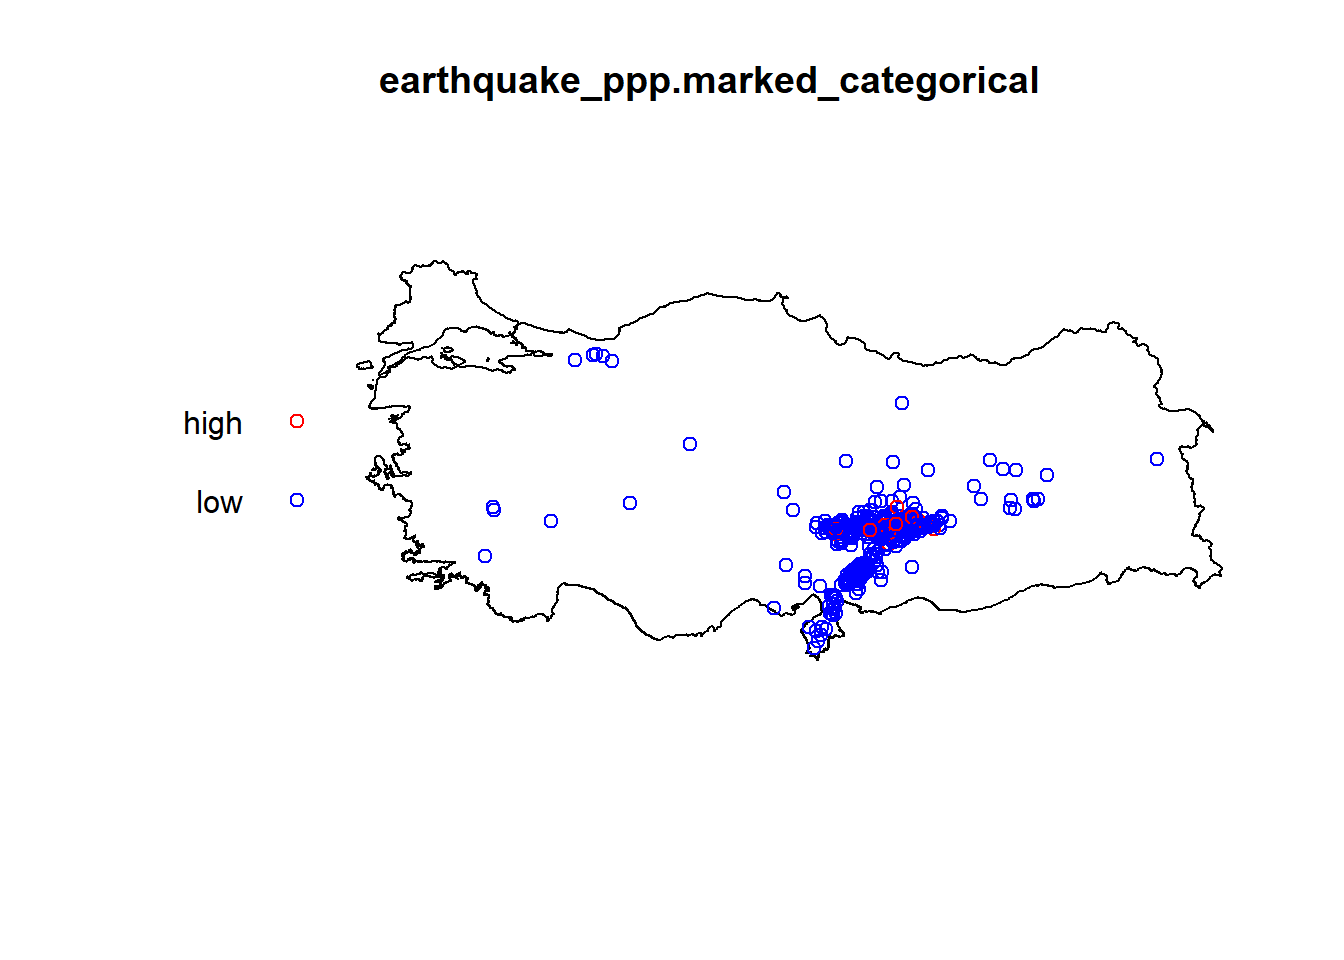
\includegraphics{Applied-Spatial-Data-Analysis_files/figure-latex/unnamed-chunk-18-2.pdf}

\url{https://rspatial.org/raster/rosu/Chapter5.html}
\url{https://geobgu.xyz/r/point-pattern-analysis.html}
\url{https://www.keene.edu/campus/maps/tool/}
\url{https://data.humdata.org/dataset/cod-ab-tur}?
\url{https://www.jla-data.net/eng/merging-geometry-of-sf-objects-in-r/}

\hypertarget{external-datasets---clinics-dataset-sa}{%
\paragraph{External Datasets - Clinics Dataset SA}\label{external-datasets---clinics-dataset-sa}}

Download the data from the following:

\url{https://web1.capetown.gov.za/web1/OpenDataPortal/DatasetDetail?DatasetName=Clinics}

\begin{Shaded}
\begin{Highlighting}[]
\FunctionTok{library}\NormalTok{(sf)}

\NormalTok{RSA\_roads }\OtherTok{=} \StringTok{"C:/Users/01438475/OneDrive {-} University of Cape Town/ASDA/DataSets/zafrds8ff5a/ZAF\_roads.shp"} \SpecialCharTok{\%\textgreater{}\%} 
  \FunctionTok{st\_read}\NormalTok{() }\SpecialCharTok{\%\textgreater{}\%} \FunctionTok{st\_transform}\NormalTok{(}\DecValTok{4326}\NormalTok{)}
\end{Highlighting}
\end{Shaded}

\begin{verbatim}
## Reading layer `ZAF_roads' from data source 
##   `C:\Users\01438475\OneDrive - University of Cape Town\ASDA\DataSets\zafrds8ff5a\ZAF_roads.shp' 
##   using driver `ESRI Shapefile'
## Simple feature collection with 5559 features and 5 fields
## Geometry type: MULTILINESTRING
## Dimension:     XY
## Bounding box:  xmin: 16.48784 ymin: -34.82747 xmax: 32.85267 ymax: -22.17693
## Geodetic CRS:  WGS 84
\end{verbatim}

\begin{Shaded}
\begin{Highlighting}[]
\NormalTok{RSA\_biome }\OtherTok{=} \StringTok{"C:/Users/01438475/OneDrive {-} University of Cape Town/ASDA/DataSets/rsabiome4xkhi/RSA\_biome.shp"} \SpecialCharTok{\%\textgreater{}\%} 
  \FunctionTok{st\_read}\NormalTok{() }\SpecialCharTok{\%\textgreater{}\%} \FunctionTok{st\_transform}\NormalTok{(}\DecValTok{4326}\NormalTok{)}
\end{Highlighting}
\end{Shaded}

\begin{verbatim}
## Reading layer `RSA_biome' from data source 
##   `C:\Users\01438475\OneDrive - University of Cape Town\ASDA\DataSets\rsabiome4xkhi\RSA_biome.shp' 
##   using driver `ESRI Shapefile'
## Simple feature collection with 3127 features and 1 field
## Geometry type: POLYGON
## Dimension:     XY
## Bounding box:  xmin: 16.45296 ymin: -34.8336 xmax: 32.8928 ymax: -22.12583
## Geodetic CRS:  Hartebeesthoek94
\end{verbatim}

\begin{Shaded}
\begin{Highlighting}[]
\NormalTok{clinics\_sf }\OtherTok{=} \StringTok{"C:/Users/01438475/OneDrive {-} University of Cape Town/ASDA/DataSets/Clinics/SL\_CLNC.shp"} \SpecialCharTok{\%\textgreater{}\%} 
  \FunctionTok{st\_read}\NormalTok{() }\SpecialCharTok{\%\textgreater{}\%} \FunctionTok{st\_transform}\NormalTok{(}\DecValTok{4326}\NormalTok{)}
\end{Highlighting}
\end{Shaded}

\begin{verbatim}
## Reading layer `SL_CLNC' from data source 
##   `C:\Users\01438475\OneDrive - University of Cape Town\ASDA\DataSets\Clinics\SL_CLNC.shp' 
##   using driver `ESRI Shapefile'
## Simple feature collection with 149 features and 5 fields
## Geometry type: POINT
## Dimension:     XY
## Bounding box:  xmin: 18.34268 ymin: -34.19491 xmax: 18.90847 ymax: -33.51262
## Geodetic CRS:  WGS 84
\end{verbatim}

\begin{Shaded}
\begin{Highlighting}[]
\NormalTok{ct.wards\_sf }\OtherTok{\textless{}{-}} \StringTok{"C:/Users/01438475/OneDrive {-} University of Cape Town/ASDA/DataSets/sa/CPT/electoral wards for cpt.shp"} \SpecialCharTok{\%\textgreater{}\%}
  \FunctionTok{st\_read}\NormalTok{(}\AttributeTok{quiet =} \ConstantTok{TRUE}\NormalTok{) }\SpecialCharTok{\%\textgreater{}\%} 
  \FunctionTok{st\_set\_crs}\NormalTok{(}\DecValTok{4326}\NormalTok{)}

\FunctionTok{st\_crs}\NormalTok{(ct.wards\_sf)}
\end{Highlighting}
\end{Shaded}

\begin{verbatim}
## Coordinate Reference System:
##   User input: EPSG:4326 
##   wkt:
## GEOGCRS["WGS 84",
##     DATUM["World Geodetic System 1984",
##         ELLIPSOID["WGS 84",6378137,298.257223563,
##             LENGTHUNIT["metre",1]]],
##     PRIMEM["Greenwich",0,
##         ANGLEUNIT["degree",0.0174532925199433]],
##     CS[ellipsoidal,2],
##         AXIS["geodetic latitude (Lat)",north,
##             ORDER[1],
##             ANGLEUNIT["degree",0.0174532925199433]],
##         AXIS["geodetic longitude (Lon)",east,
##             ORDER[2],
##             ANGLEUNIT["degree",0.0174532925199433]],
##     USAGE[
##         SCOPE["Horizontal component of 3D system."],
##         AREA["World."],
##         BBOX[-90,-180,90,180]],
##     ID["EPSG",4326]]
\end{verbatim}

\begin{Shaded}
\begin{Highlighting}[]
\FunctionTok{st\_crs}\NormalTok{(clinics\_sf)}
\end{Highlighting}
\end{Shaded}

\begin{verbatim}
## Coordinate Reference System:
##   User input: EPSG:4326 
##   wkt:
## GEOGCRS["WGS 84",
##     DATUM["World Geodetic System 1984",
##         ELLIPSOID["WGS 84",6378137,298.257223563,
##             LENGTHUNIT["metre",1]]],
##     PRIMEM["Greenwich",0,
##         ANGLEUNIT["degree",0.0174532925199433]],
##     CS[ellipsoidal,2],
##         AXIS["geodetic latitude (Lat)",north,
##             ORDER[1],
##             ANGLEUNIT["degree",0.0174532925199433]],
##         AXIS["geodetic longitude (Lon)",east,
##             ORDER[2],
##             ANGLEUNIT["degree",0.0174532925199433]],
##     USAGE[
##         SCOPE["Horizontal component of 3D system."],
##         AREA["World."],
##         BBOX[-90,-180,90,180]],
##     ID["EPSG",4326]]
\end{verbatim}

\begin{Shaded}
\begin{Highlighting}[]
\FunctionTok{class}\NormalTok{(clinics\_sf)}
\end{Highlighting}
\end{Shaded}

\begin{verbatim}
## [1] "sf"         "data.frame"
\end{verbatim}

\begin{Shaded}
\begin{Highlighting}[]
\FunctionTok{summary}\NormalTok{(clinics\_sf)}
\end{Highlighting}
\end{Shaded}

\begin{verbatim}
##      LCTN               ATHY               NAME              CLASS          
##  Length:149         Length:149         Length:149         Length:149        
##  Class :character   Class :character   Class :character   Class :character  
##  Mode  :character   Mode  :character   Mode  :character   Mode  :character  
##      RGN                     geometry  
##  Length:149         POINT        :149  
##  Class :character   epsg:4326    :  0  
##  Mode  :character   +proj=long...:  0
\end{verbatim}

\hypertarget{swedishpines-dataset-from-spatstat.data-library-1}{%
\subsection{Swedishpines Dataset from spatstat.data library}\label{swedishpines-dataset-from-spatstat.data-library-1}}

\begin{Shaded}
\begin{Highlighting}[]
\FunctionTok{data}\NormalTok{(swedishpines)}
\NormalTok{swp }\OtherTok{=} \FunctionTok{rescale.ppp}\NormalTok{(swedishpines)}
\FunctionTok{class}\NormalTok{(swp)}
\end{Highlighting}
\end{Shaded}

\begin{Shaded}
\begin{Highlighting}[]
\NormalTok{\#\# [1] "ppp"}
\end{Highlighting}
\end{Shaded}

\begin{Shaded}
\begin{Highlighting}[]
\FunctionTok{summary}\NormalTok{(swp)}
\end{Highlighting}
\end{Shaded}

\begin{Shaded}
\begin{Highlighting}[]
\NormalTok{\#\# Planar point pattern:  71 points}
\NormalTok{\#\# Average intensity 0.7395833 points per square metre}
\NormalTok{\#\# }
\NormalTok{\#\# Coordinates are given to 1 decimal place}
\NormalTok{\#\# i.e. rounded to the nearest multiple of 0.1 metres}
\NormalTok{\#\# }
\NormalTok{\#\# Window: rectangle = [0, 9.6] x [0, 10] metres}
\NormalTok{\#\# Window area = 96 square metres}
\NormalTok{\#\# Unit of length: 1 metre}
\end{Highlighting}
\end{Shaded}

\begin{Shaded}
\begin{Highlighting}[]
\FunctionTok{plot}\NormalTok{(swp)}
\end{Highlighting}
\end{Shaded}

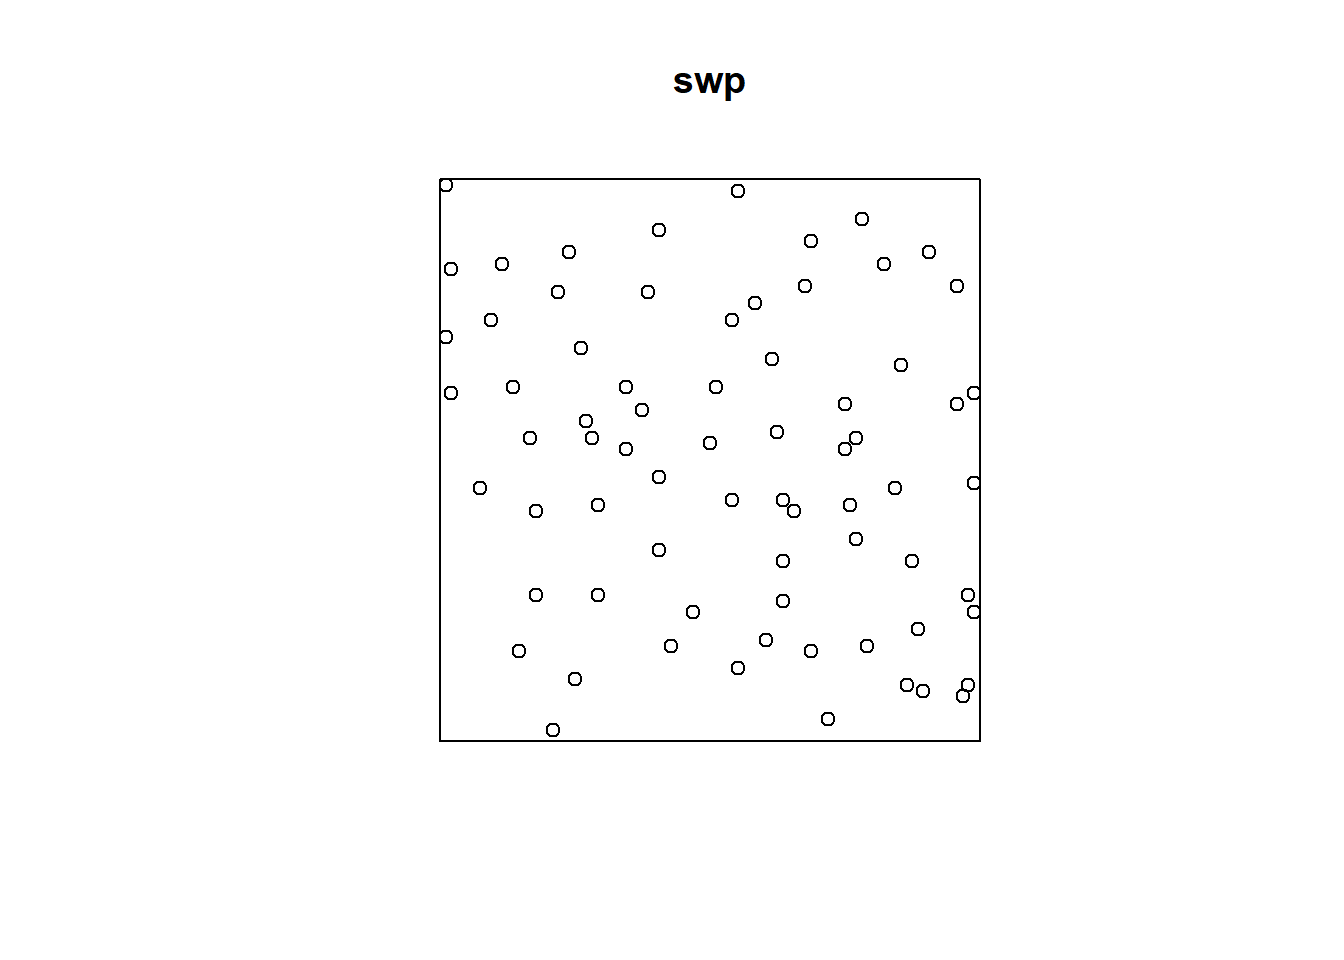
\includegraphics{Applied-Spatial-Data-Analysis_files/figure-latex/unnamed-chunk-20-1.pdf}

\hypertarget{clinics-dataset-using-simple-features-sf}{%
\subsection{Clinics Dataset Using Simple Features (SF)}\label{clinics-dataset-using-simple-features-sf}}

Download the data from the following:

\url{https://web1.capetown.gov.za/web1/OpenDataPortal/DatasetDetail?DatasetName=Clinics}

Extract the data frame into R:

\begin{Shaded}
\begin{Highlighting}[]
\FunctionTok{library}\NormalTok{(sf)}
\NormalTok{clinics\_sf }\OtherTok{=} \FunctionTok{st\_read}\NormalTok{(}\StringTok{"C:/Users/01438475/OneDrive {-} University of Cape Town/ASDA/DataSets/Clinics/SL\_CLNC.shp"}\NormalTok{)}
\end{Highlighting}
\end{Shaded}

\begin{verbatim}
## Reading layer `SL_CLNC' from data source 
##   `C:\Users\01438475\OneDrive - University of Cape Town\ASDA\DataSets\Clinics\SL_CLNC.shp' 
##   using driver `ESRI Shapefile'
## Simple feature collection with 149 features and 5 fields
## Geometry type: POINT
## Dimension:     XY
## Bounding box:  xmin: 18.34268 ymin: -34.19491 xmax: 18.90847 ymax: -33.51262
## Geodetic CRS:  WGS 84
\end{verbatim}

\begin{Shaded}
\begin{Highlighting}[]
\NormalTok{clinics\_sf}
\end{Highlighting}
\end{Shaded}

\begin{verbatim}
## Simple feature collection with 149 features and 5 fields
## Geometry type: POINT
## Dimension:     XY
## Bounding box:  xmin: 18.34268 ymin: -34.19491 xmax: 18.90847 ymax: -33.51262
## Geodetic CRS:  WGS 84
## First 10 features:
##                                        LCTN              ATHY
## 1           C/O Adam/ Liedeman Street Mamre              PAWC
## 2                 Cnr Hermes & GrosvenorAve CITY OF CAPE TOWN
## 3            Hassen Kahn Ave Rusthof Strand              PAWC
## 4              61 Central Circle, Fish Hoek CITY OF CAPE TOWN
## 5                     Simon Street, Nomzamo CITY OF CAPE TOWN
## 6  C/O Musical and Hospital Street Macassar              PAWC
## 7            28 Church Street Somerset West CITY OF CAPE TOWN
## 8                       Fagan Street Strand CITY OF CAPE TOWN
## 9    Karbonkel Road, CMC Building, Hout Bay              PAWC
## 10                Midmar Street Groenvallei CITY OF CAPE TOWN
##                      NAME                CLASS       RGN
## 1               MAMRE CDC Community Day Centre   Western
## 2        SAXON SEA CLINIC               Clinic   Western
## 3            GUSTROUW CDC Community Day Centre   Eastern
## 4        FISH HOEK CLINIC               Clinic  Southern
## 5              IKWEZI CDC Community Day Centre   Eastern
## 6            MACASSAR CDC Community Day Centre   Eastern
## 7    SOMERSET WEST CLINIC               Clinic   Eastern
## 8  FAGAN STREET SATELLITE            Satellite   Eastern
## 9    HOUT BAY HARBOUR CDC Community Day Centre  Southern
## 10  GROENVALLEI SATELLITE            Satellite Tygerberg
##                      geometry
## 1  POINT (18.47692 -33.51262)
## 2  POINT (18.48881 -33.55012)
## 3  POINT (18.85211 -34.13472)
## 4  POINT (18.42632 -34.13669)
## 5  POINT (18.86622 -34.11375)
## 6  POINT (18.76369 -34.06105)
## 7  POINT (18.84814 -34.08579)
## 8   POINT (18.82979 -34.1162)
## 9   POINT (18.34268 -34.0549)
## 10 POINT (18.66701 -33.89165)
\end{verbatim}

\begin{Shaded}
\begin{Highlighting}[]
\FunctionTok{class}\NormalTok{(clinics\_sf)}
\end{Highlighting}
\end{Shaded}

\begin{verbatim}
## [1] "sf"         "data.frame"
\end{verbatim}

\begin{Shaded}
\begin{Highlighting}[]
\FunctionTok{summary}\NormalTok{(clinics\_sf)}
\end{Highlighting}
\end{Shaded}

\begin{verbatim}
##      LCTN               ATHY               NAME              CLASS          
##  Length:149         Length:149         Length:149         Length:149        
##  Class :character   Class :character   Class :character   Class :character  
##  Mode  :character   Mode  :character   Mode  :character   Mode  :character  
##      RGN                     geometry  
##  Length:149         POINT        :149  
##  Class :character   epsg:4326    :  0  
##  Mode  :character   +proj=long...:  0
\end{verbatim}

\hypertarget{plotting-datasets}{%
\section{Plotting Datasets}\label{plotting-datasets}}

\hypertarget{basic-plot-function}{%
\subsection{Basic plot() function}\label{basic-plot-function}}

\begin{Shaded}
\begin{Highlighting}[]
\FunctionTok{plot}\NormalTok{(swp)}
\end{Highlighting}
\end{Shaded}

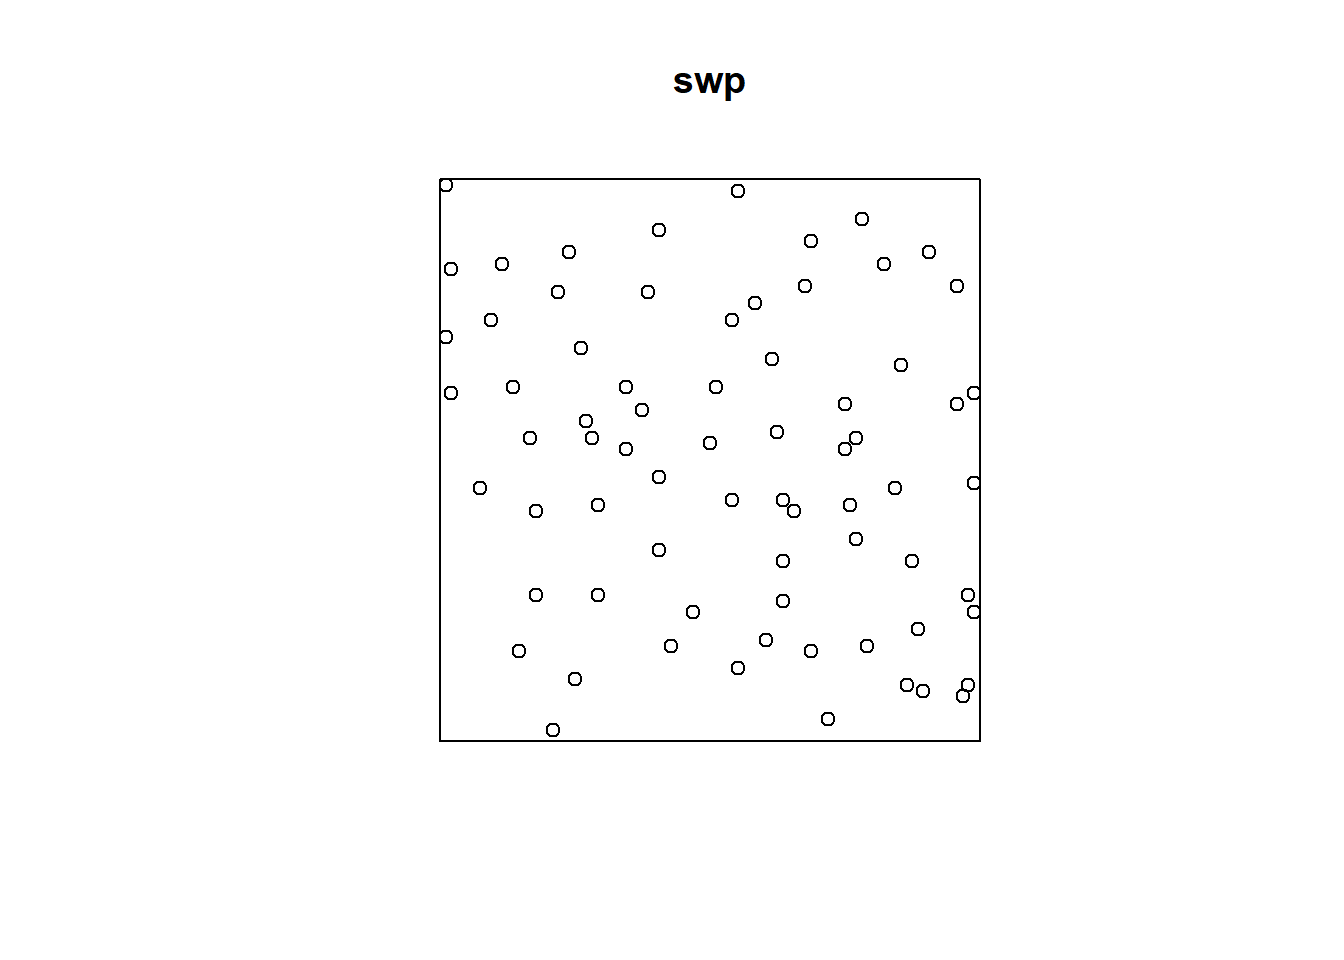
\includegraphics{Applied-Spatial-Data-Analysis_files/figure-latex/unnamed-chunk-22-1.pdf}

\hypertarget{basic-ggplot-function---sf-object}{%
\subsection{Basic ggplot() function - (sf) object}\label{basic-ggplot-function---sf-object}}

\begin{Shaded}
\begin{Highlighting}[]
\FunctionTok{library}\NormalTok{(ggplot2)}
\NormalTok{plot1 }\OtherTok{=} \FunctionTok{ggplot}\NormalTok{() }\SpecialCharTok{+} 
  \FunctionTok{geom\_sf}\NormalTok{(}\AttributeTok{data =}\NormalTok{ clinics\_sf, }\AttributeTok{size =}\NormalTok{ .}\DecValTok{8}\NormalTok{, }\AttributeTok{color =} \StringTok{"black"}\NormalTok{) }\SpecialCharTok{+} 
  \FunctionTok{ggtitle}\NormalTok{(}\StringTok{"Location of Cape Town clinics {-} 2016"}\NormalTok{) }\SpecialCharTok{+} 
  \CommentTok{\# not specifying crs here, coord\_sf will use the CRS defined in the first layer = "+proj=longlat +datum=WGS84 +no\_defs"}
  \FunctionTok{coord\_sf}\NormalTok{() }
\NormalTok{plot1}
\end{Highlighting}
\end{Shaded}

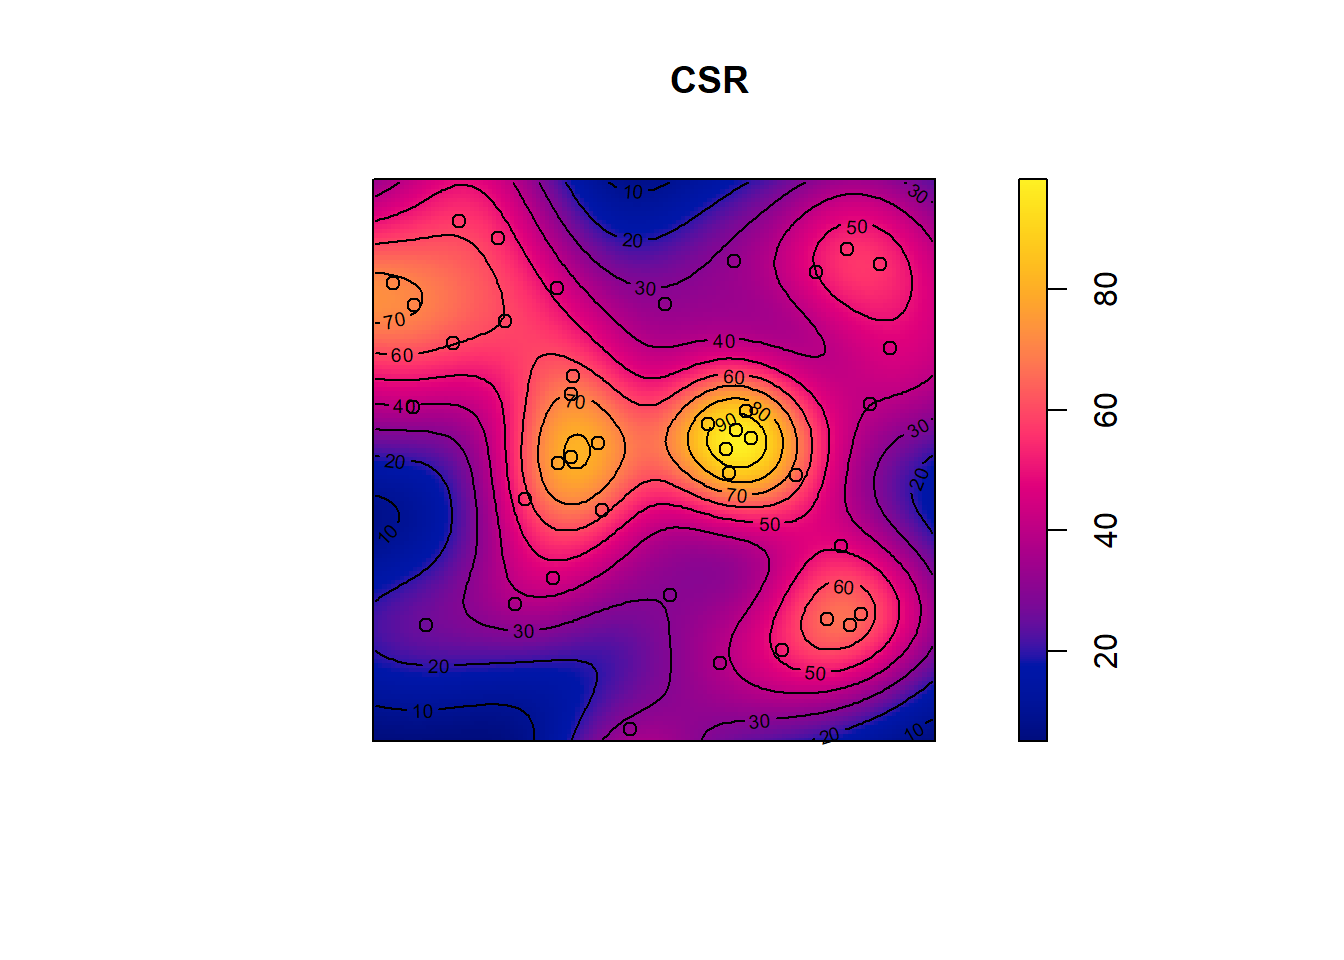
\includegraphics{Applied-Spatial-Data-Analysis_files/figure-latex/unnamed-chunk-23-1.pdf}

\hypertarget{ggplot-function-with-a-bounding-box---sf-object}{%
\subsection{ggplot() function with a bounding box - (sf) object}\label{ggplot-function-with-a-bounding-box---sf-object}}

\begin{Shaded}
\begin{Highlighting}[]
\FunctionTok{library}\NormalTok{(ggplot2)}
\NormalTok{plot2 }\OtherTok{=} \FunctionTok{ggplot}\NormalTok{() }\SpecialCharTok{+} 
  \FunctionTok{geom\_sf}\NormalTok{(}\AttributeTok{data =}\NormalTok{ clinics\_sf, }\AttributeTok{size =}\NormalTok{ .}\DecValTok{8}\NormalTok{, }\AttributeTok{color =} \StringTok{"black"}\NormalTok{) }\SpecialCharTok{+} 
  \FunctionTok{ggtitle}\NormalTok{(}\StringTok{"Location of Cape Town clinics {-} 2016"}\NormalTok{) }\SpecialCharTok{+} 
  \FunctionTok{coord\_sf}\NormalTok{(}\AttributeTok{xlim =} \FunctionTok{c}\NormalTok{(}\FloatTok{18.34}\NormalTok{, }\FloatTok{18.91}\NormalTok{), }\AttributeTok{ylim =} \FunctionTok{c}\NormalTok{(}\SpecialCharTok{{-}}\FloatTok{34.19}\NormalTok{, }\SpecialCharTok{{-}}\FloatTok{33.51262}\NormalTok{)) }\SpecialCharTok{+}
  \FunctionTok{theme}\NormalTok{(}\AttributeTok{panel.grid.major =} \FunctionTok{element\_blank}\NormalTok{(), }
        \AttributeTok{panel.grid.minor =} \FunctionTok{element\_blank}\NormalTok{(),}
        \AttributeTok{panel.background =} \FunctionTok{element\_rect}\NormalTok{(}\AttributeTok{colour =} \StringTok{"black"}\NormalTok{, }\AttributeTok{size=}\DecValTok{1}\NormalTok{, }\AttributeTok{fill=}\ConstantTok{NA}\NormalTok{))}
\end{Highlighting}
\end{Shaded}

\begin{verbatim}
## Warning: The `size` argument of `element_rect()` is deprecated as of ggplot2 3.4.0.
## i Please use the `linewidth` argument instead.
\end{verbatim}

\begin{Shaded}
\begin{Highlighting}[]
\NormalTok{plot2}
\end{Highlighting}
\end{Shaded}

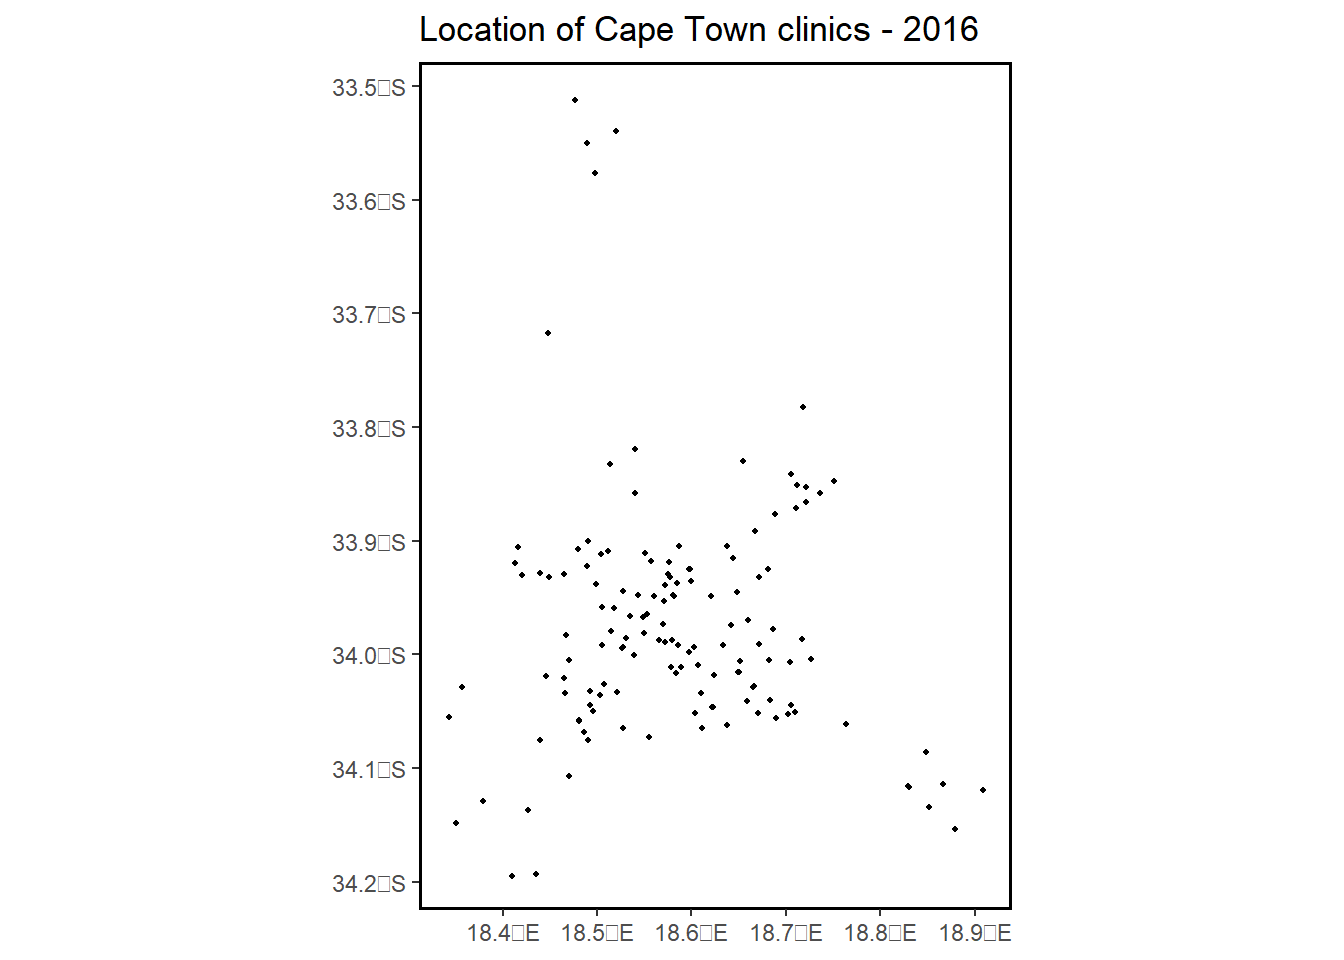
\includegraphics{Applied-Spatial-Data-Analysis_files/figure-latex/unnamed-chunk-24-1.pdf}

\hypertarget{ggplot-with-electoral-wards-shape-file}{%
\subsection{ggplot() with Electoral Wards Shape File}\label{ggplot-with-electoral-wards-shape-file}}

In order to plot using the electoral wards polygons, we need the sf data frame to be converted into Spatial Points Data Frame (sp).

\begin{Shaded}
\begin{Highlighting}[]
\NormalTok{clinics\_sp }\OtherTok{\textless{}{-}} \FunctionTok{as}\NormalTok{(clinics\_sf, }\AttributeTok{Class =} \StringTok{"Spatial"}\NormalTok{)}
\FunctionTok{class}\NormalTok{(clinics\_sp)}
\end{Highlighting}
\end{Shaded}

\begin{verbatim}
## [1] "SpatialPointsDataFrame"
## attr(,"package")
## [1] "sp"
\end{verbatim}

Download the CPT electoral wards and import the shape file as follows:

\begin{Shaded}
\begin{Highlighting}[]
\FunctionTok{library}\NormalTok{(sf)}
\NormalTok{ct.wards\_sf }\OtherTok{=} \FunctionTok{st\_read}\NormalTok{(}\StringTok{"C:/Users/01438475/OneDrive {-} University of Cape Town/ASDA/DataSets/sa/CPT/electoral wards for cpt.shp"}\NormalTok{)}
\end{Highlighting}
\end{Shaded}

\begin{verbatim}
## Reading layer `electoral wards for cpt' from data source 
##   `C:\Users\01438475\OneDrive - University of Cape Town\ASDA\DataSets\sa\CPT\electoral wards for cpt.shp' 
##   using driver `ESRI Shapefile'
## Simple feature collection with 111 features and 9 fields
## Geometry type: MULTIPOLYGON
## Dimension:     XY
## Bounding box:  xmin: 18.30722 ymin: -34.35834 xmax: 19.00467 ymax: -33.47128
## CRS:           NA
\end{verbatim}

\begin{Shaded}
\begin{Highlighting}[]
\FunctionTok{st\_geometry\_type}\NormalTok{(ct.wards\_sf)}
\end{Highlighting}
\end{Shaded}

\begin{verbatim}
##   [1] MULTIPOLYGON MULTIPOLYGON MULTIPOLYGON MULTIPOLYGON MULTIPOLYGON
##   [6] MULTIPOLYGON MULTIPOLYGON MULTIPOLYGON MULTIPOLYGON MULTIPOLYGON
##  [11] MULTIPOLYGON MULTIPOLYGON MULTIPOLYGON MULTIPOLYGON MULTIPOLYGON
##  [16] MULTIPOLYGON MULTIPOLYGON MULTIPOLYGON MULTIPOLYGON MULTIPOLYGON
##  [21] MULTIPOLYGON MULTIPOLYGON MULTIPOLYGON MULTIPOLYGON MULTIPOLYGON
##  [26] MULTIPOLYGON MULTIPOLYGON MULTIPOLYGON MULTIPOLYGON MULTIPOLYGON
##  [31] MULTIPOLYGON MULTIPOLYGON MULTIPOLYGON MULTIPOLYGON MULTIPOLYGON
##  [36] MULTIPOLYGON MULTIPOLYGON MULTIPOLYGON MULTIPOLYGON MULTIPOLYGON
##  [41] MULTIPOLYGON MULTIPOLYGON MULTIPOLYGON MULTIPOLYGON MULTIPOLYGON
##  [46] MULTIPOLYGON MULTIPOLYGON MULTIPOLYGON MULTIPOLYGON MULTIPOLYGON
##  [51] MULTIPOLYGON MULTIPOLYGON MULTIPOLYGON MULTIPOLYGON MULTIPOLYGON
##  [56] MULTIPOLYGON MULTIPOLYGON MULTIPOLYGON MULTIPOLYGON MULTIPOLYGON
##  [61] MULTIPOLYGON MULTIPOLYGON MULTIPOLYGON MULTIPOLYGON MULTIPOLYGON
##  [66] MULTIPOLYGON MULTIPOLYGON MULTIPOLYGON MULTIPOLYGON MULTIPOLYGON
##  [71] MULTIPOLYGON MULTIPOLYGON MULTIPOLYGON MULTIPOLYGON MULTIPOLYGON
##  [76] MULTIPOLYGON MULTIPOLYGON MULTIPOLYGON MULTIPOLYGON MULTIPOLYGON
##  [81] MULTIPOLYGON MULTIPOLYGON MULTIPOLYGON MULTIPOLYGON MULTIPOLYGON
##  [86] MULTIPOLYGON MULTIPOLYGON MULTIPOLYGON MULTIPOLYGON MULTIPOLYGON
##  [91] MULTIPOLYGON MULTIPOLYGON MULTIPOLYGON MULTIPOLYGON MULTIPOLYGON
##  [96] MULTIPOLYGON MULTIPOLYGON MULTIPOLYGON MULTIPOLYGON MULTIPOLYGON
## [101] MULTIPOLYGON MULTIPOLYGON MULTIPOLYGON MULTIPOLYGON MULTIPOLYGON
## [106] MULTIPOLYGON MULTIPOLYGON MULTIPOLYGON MULTIPOLYGON MULTIPOLYGON
## [111] MULTIPOLYGON
## 18 Levels: GEOMETRY POINT LINESTRING POLYGON MULTIPOINT ... TRIANGLE
\end{verbatim}

\begin{Shaded}
\begin{Highlighting}[]
\FunctionTok{library}\NormalTok{(ggplot2)}
\FunctionTok{ggplot}\NormalTok{() }\SpecialCharTok{+} 
  \FunctionTok{geom\_sf}\NormalTok{(}\AttributeTok{data =}\NormalTok{ ct.wards\_sf, }\AttributeTok{size =}\NormalTok{ .}\DecValTok{5}\NormalTok{, }\AttributeTok{color =} \StringTok{"black"}\NormalTok{) }\SpecialCharTok{+} 
  \FunctionTok{geom\_point}\NormalTok{(}\FunctionTok{aes}\NormalTok{(}\AttributeTok{x =}\NormalTok{ clinics\_sp}\SpecialCharTok{@}\NormalTok{coords[,}\DecValTok{1}\NormalTok{], }\AttributeTok{y =}\NormalTok{ clinics\_sp}\SpecialCharTok{@}\NormalTok{coords[,}\DecValTok{2}\NormalTok{]),}
             \AttributeTok{data =}\NormalTok{ clinics\_sp}\SpecialCharTok{@}\NormalTok{data, }\AttributeTok{alpha =} \DecValTok{1}\NormalTok{,}\AttributeTok{size=}\DecValTok{2}\NormalTok{, }\AttributeTok{color =} \StringTok{"red"}\NormalTok{)}\SpecialCharTok{+} 
  \FunctionTok{ggtitle}\NormalTok{(}\StringTok{"Spatial locations of Cape Town clinics within wards"}\NormalTok{) }\SpecialCharTok{+} 
  \FunctionTok{coord\_sf}\NormalTok{()}
\end{Highlighting}
\end{Shaded}

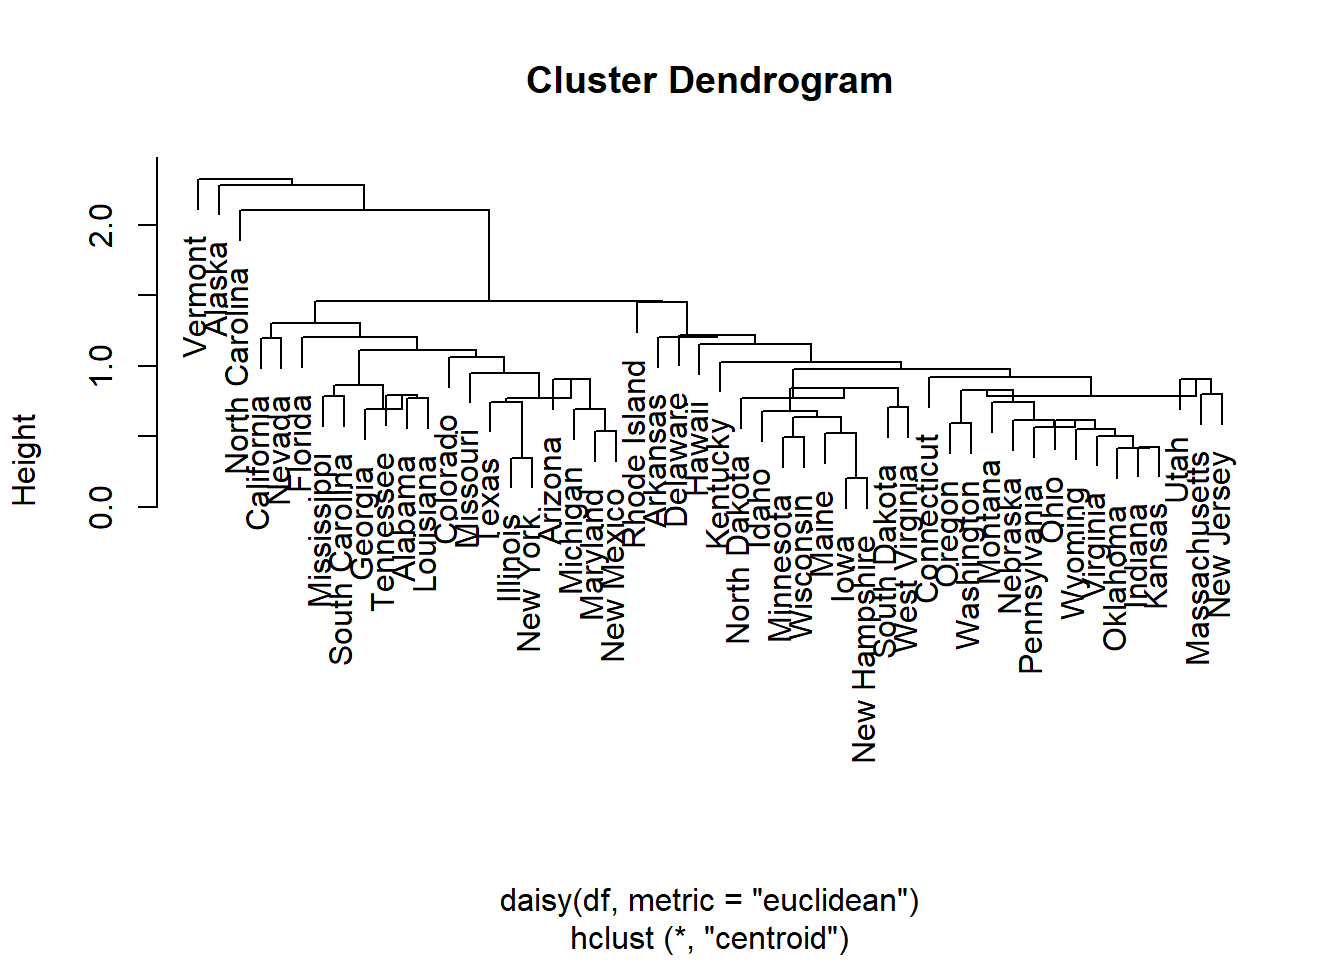
\includegraphics{Applied-Spatial-Data-Analysis_files/figure-latex/unnamed-chunk-26-1.pdf}

\hypertarget{quadrat-analysis---quadrat-counts-and-tests}{%
\section{Quadrat Analysis - Quadrat Counts and Tests}\label{quadrat-analysis---quadrat-counts-and-tests}}

\hypertarget{turkey-earthquake}{%
\subsection{Turkey Earthquake}\label{turkey-earthquake}}

\begin{Shaded}
\begin{Highlighting}[]
\NormalTok{q }\OtherTok{=} \FunctionTok{quadratcount}\NormalTok{(earthquake\_ppp, }\AttributeTok{nx =} \DecValTok{7}\NormalTok{, }\AttributeTok{ny =} \DecValTok{7}\NormalTok{)}
\FunctionTok{plot}\NormalTok{(q)}
\end{Highlighting}
\end{Shaded}

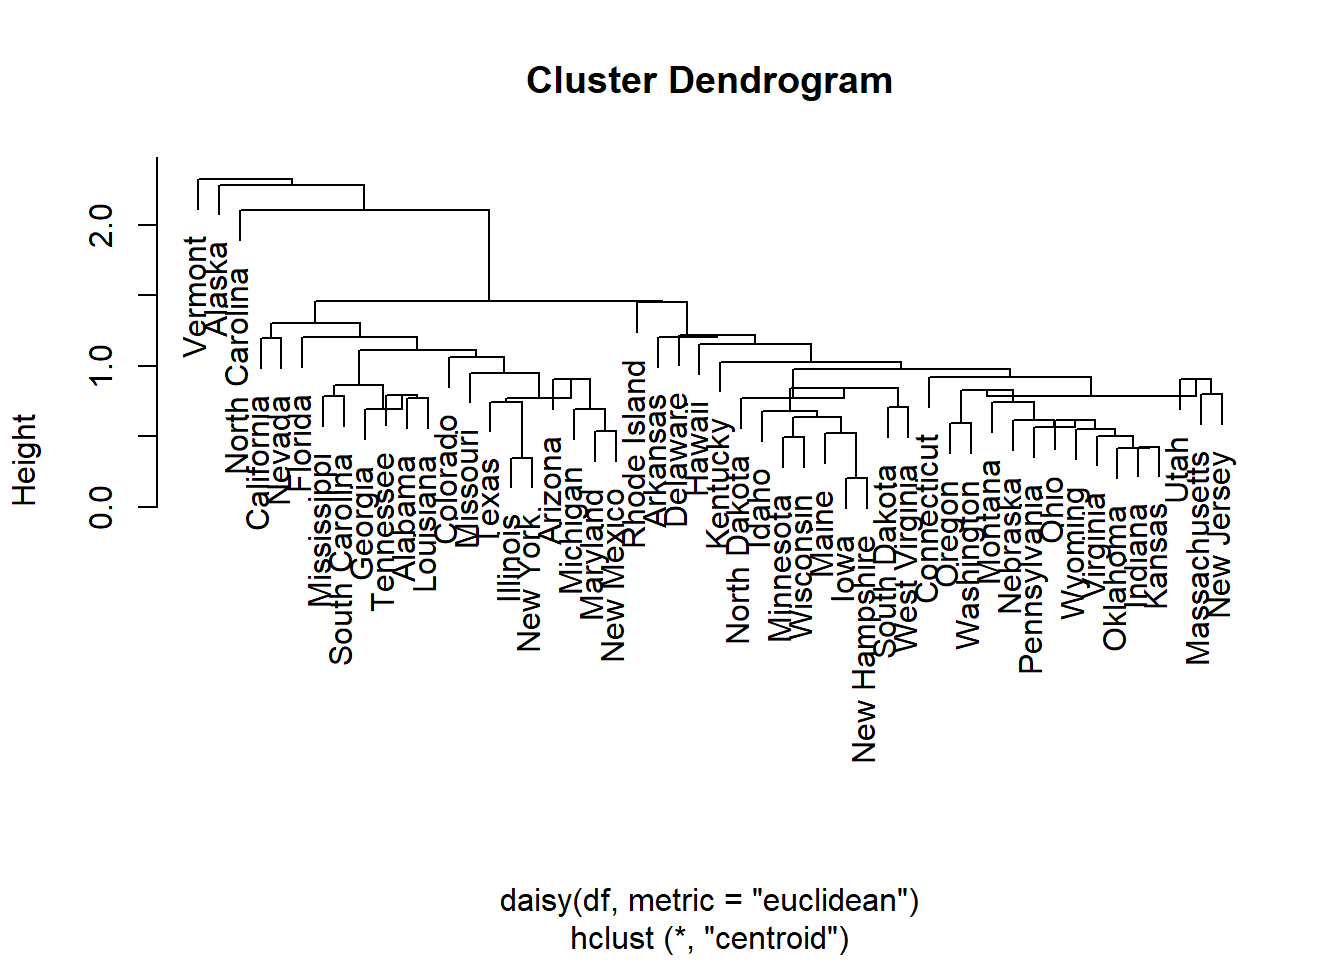
\includegraphics{Applied-Spatial-Data-Analysis_files/figure-latex/unnamed-chunk-27-1.pdf}

\begin{Shaded}
\begin{Highlighting}[]
\NormalTok{den }\OtherTok{=} \FunctionTok{density}\NormalTok{(earthquake\_ppp)}
\FunctionTok{plot}\NormalTok{(den)}
\end{Highlighting}
\end{Shaded}

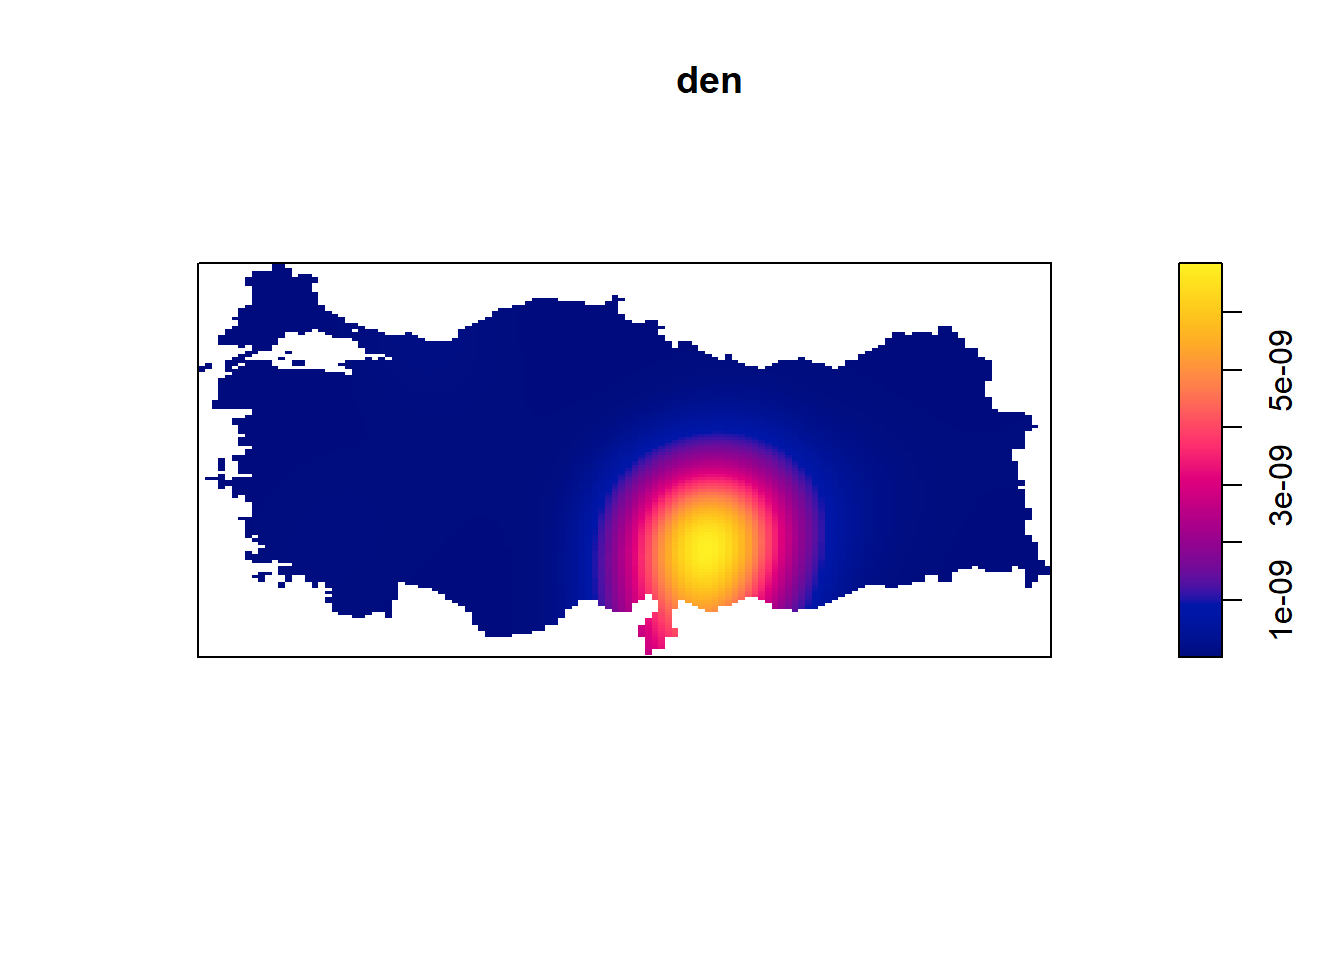
\includegraphics{Applied-Spatial-Data-Analysis_files/figure-latex/unnamed-chunk-27-2.pdf}

\hypertarget{swp-dataset}{%
\subsection{swp dataset}\label{swp-dataset}}

Quadrat counts:

\begin{Shaded}
\begin{Highlighting}[]
\NormalTok{Q3x3 }\OtherTok{=} \FunctionTok{quadratcount}\NormalTok{(swp, }\AttributeTok{nx=}\DecValTok{3}\NormalTok{, }\AttributeTok{ny=}\DecValTok{3}\NormalTok{)}
\FunctionTok{plot}\NormalTok{(swp)}
\FunctionTok{plot}\NormalTok{(Q3x3, }\AttributeTok{add=}\ConstantTok{TRUE}\NormalTok{, }\AttributeTok{col=}\StringTok{"red"}\NormalTok{, }\AttributeTok{cex=}\FloatTok{1.5}\NormalTok{, }\AttributeTok{lty=}\DecValTok{2}\NormalTok{)}
\end{Highlighting}
\end{Shaded}

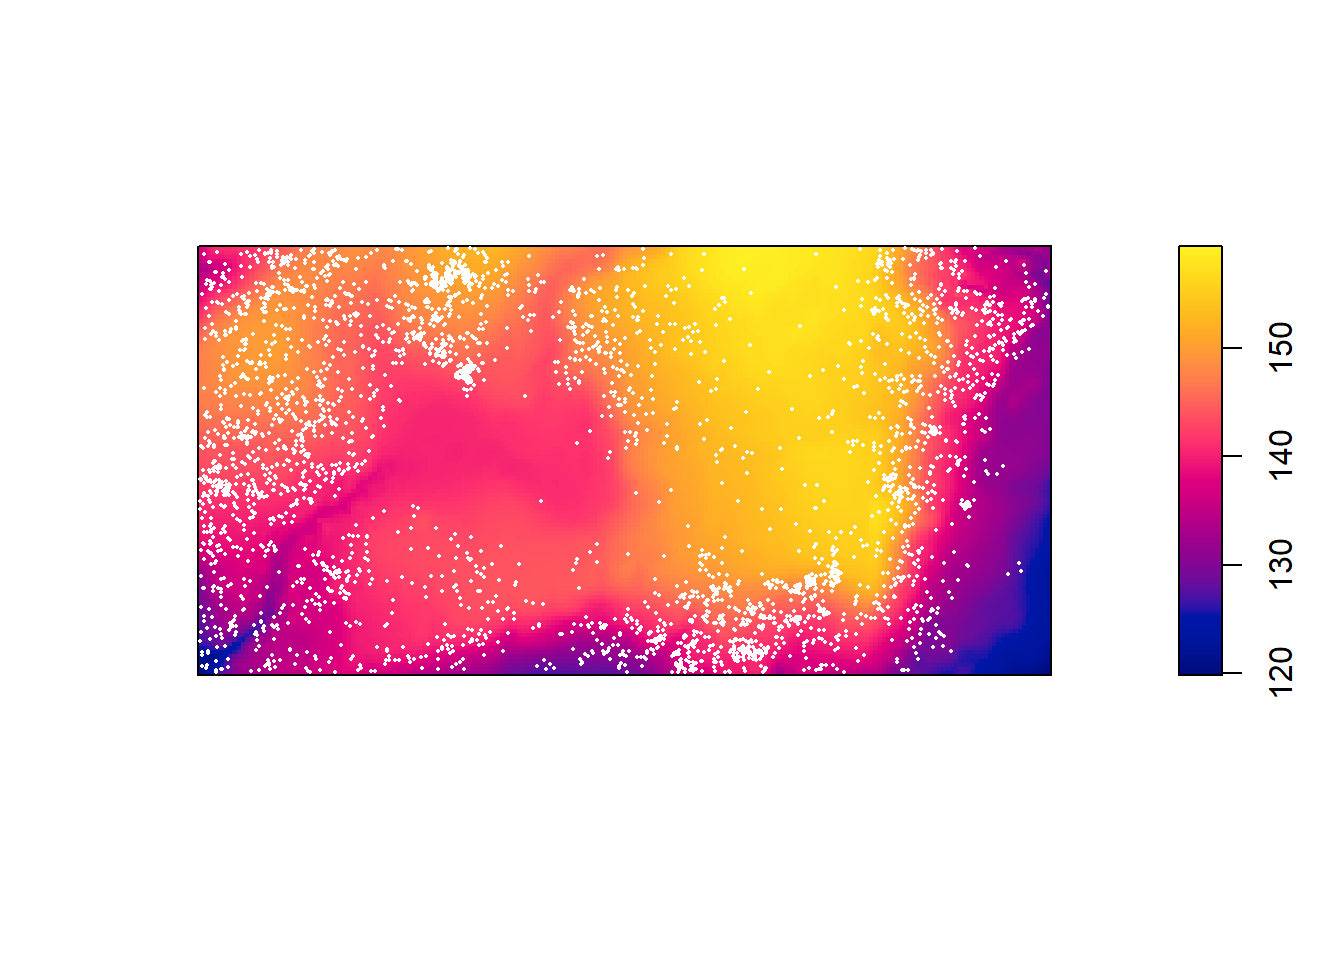
\includegraphics{Applied-Spatial-Data-Analysis_files/figure-latex/unnamed-chunk-28-1.pdf}

\begin{Shaded}
\begin{Highlighting}[]
\CommentTok{\# Plot the density}
\NormalTok{cl }\OtherTok{\textless{}{-}}  \FunctionTok{interp.colours}\NormalTok{(}\FunctionTok{c}\NormalTok{(}\StringTok{"lightyellow"}\NormalTok{, }\StringTok{"orange"}\NormalTok{ ,}\StringTok{"red"}\NormalTok{), }\DecValTok{20}\NormalTok{)}

\FunctionTok{plot}\NormalTok{( }\FunctionTok{intensity}\NormalTok{(Q3x3, }\AttributeTok{image=}\ConstantTok{TRUE}\NormalTok{), }\AttributeTok{las=}\DecValTok{1}\NormalTok{, }\AttributeTok{col=}\NormalTok{cl, }\AttributeTok{main=}\ConstantTok{NULL}\NormalTok{)}
\FunctionTok{plot}\NormalTok{(swp, }\AttributeTok{pch=}\DecValTok{20}\NormalTok{, }\AttributeTok{cex=}\FloatTok{0.6}\NormalTok{, }\AttributeTok{col=}\StringTok{"black"}\NormalTok{, }\AttributeTok{add=}\ConstantTok{TRUE}\NormalTok{)  }\CommentTok{\# Add points}
\end{Highlighting}
\end{Shaded}

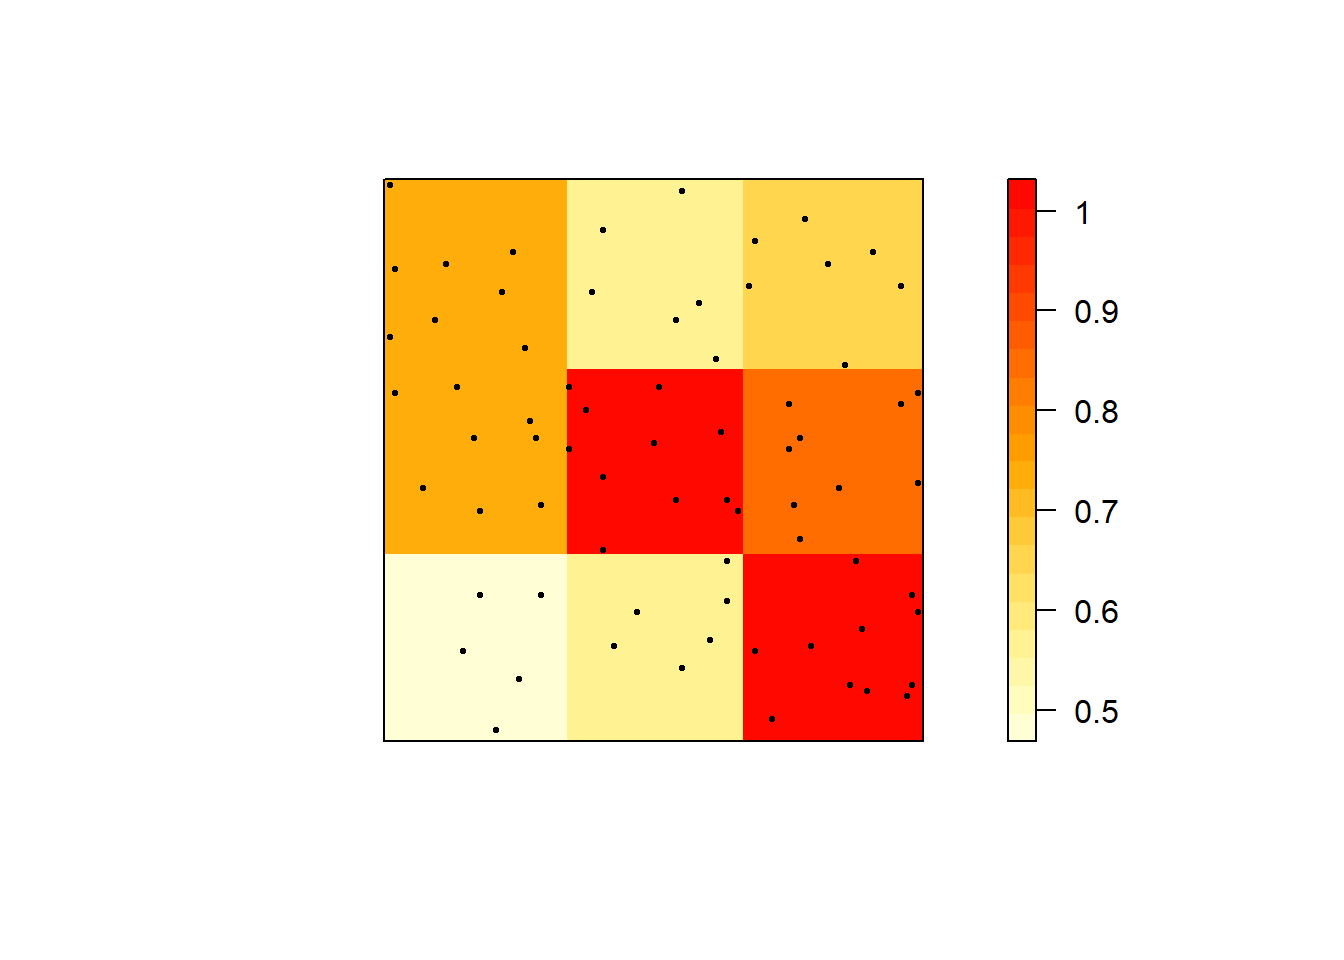
\includegraphics{Applied-Spatial-Data-Analysis_files/figure-latex/unnamed-chunk-28-2.pdf}

Quadrat test

\begin{Shaded}
\begin{Highlighting}[]
\NormalTok{Q3x3test }\OtherTok{=} \FunctionTok{quadrat.test}\NormalTok{(swp, }\DecValTok{3}\NormalTok{,}\DecValTok{3}\NormalTok{)}
\NormalTok{Q3x3test}
\end{Highlighting}
\end{Shaded}

\begin{verbatim}
## 
##  Chi-squared test of CSR using quadrat counts
## 
## data:  swp
## X2 = 4.6761, df = 8, p-value = 0.4169
## alternative hypothesis: two.sided
## 
## Quadrats: 3 by 3 grid of tiles
\end{verbatim}

\hypertarget{simulated-csr-pattern}{%
\subsection{Simulated CSR Pattern}\label{simulated-csr-pattern}}

\begin{Shaded}
\begin{Highlighting}[]
\NormalTok{Q3x3\_csr }\OtherTok{=} \FunctionTok{quadratcount}\NormalTok{(pp\_csr, }\AttributeTok{nx=}\DecValTok{3}\NormalTok{, }\AttributeTok{ny=}\DecValTok{3}\NormalTok{)}
\FunctionTok{plot}\NormalTok{(pp\_csr)}
\FunctionTok{plot}\NormalTok{(Q3x3\_csr, }\AttributeTok{add=}\ConstantTok{TRUE}\NormalTok{, }\AttributeTok{col=}\StringTok{"red"}\NormalTok{, }\AttributeTok{cex=}\FloatTok{1.5}\NormalTok{, }\AttributeTok{lty=}\DecValTok{2}\NormalTok{)}
\end{Highlighting}
\end{Shaded}

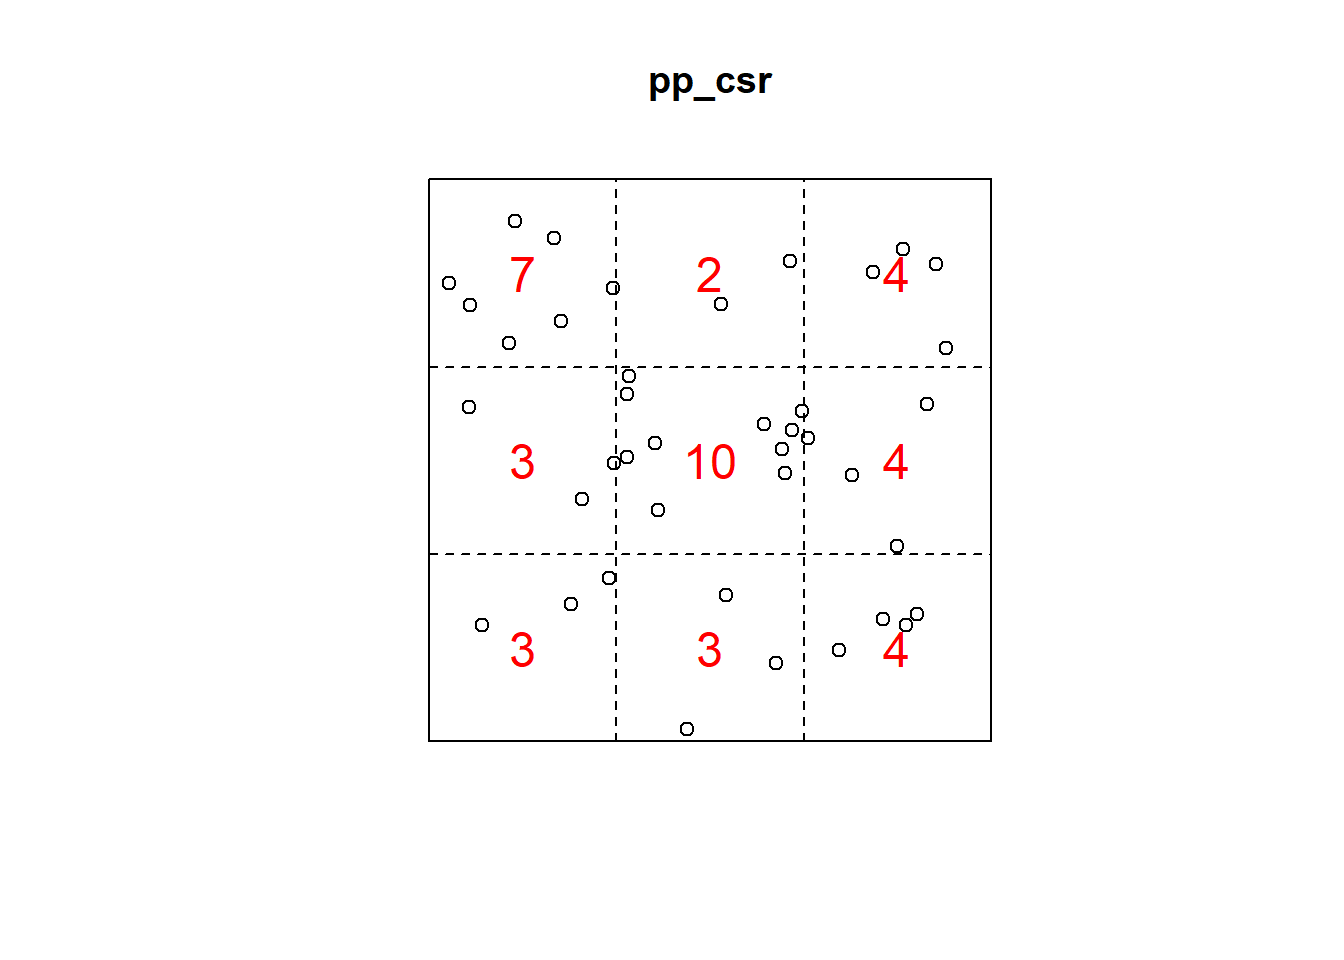
\includegraphics{Applied-Spatial-Data-Analysis_files/figure-latex/unnamed-chunk-30-1.pdf}

Test:

\begin{Shaded}
\begin{Highlighting}[]
\NormalTok{Q3x3test\_csr }\OtherTok{=} \FunctionTok{quadrat.test}\NormalTok{(pp\_csr, }\DecValTok{3}\NormalTok{,}\DecValTok{3}\NormalTok{)}
\end{Highlighting}
\end{Shaded}

\begin{verbatim}
## Warning: Some expected counts are small; chi^2 approximation may be inaccurate
\end{verbatim}

\begin{Shaded}
\begin{Highlighting}[]
\NormalTok{Q3x3test\_csr}
\end{Highlighting}
\end{Shaded}

\begin{verbatim}
## 
##  Chi-squared test of CSR using quadrat counts
## 
## data:  pp_csr
## X2 = 11.3, df = 8, p-value = 0.3705
## alternative hypothesis: two.sided
## 
## Quadrats: 3 by 3 grid of tiles
\end{verbatim}

\hypertarget{simulated-cluster-pattern}{%
\subsection{Simulated Cluster Pattern}\label{simulated-cluster-pattern}}

\begin{Shaded}
\begin{Highlighting}[]
\NormalTok{Q3x3\_cluster }\OtherTok{=} \FunctionTok{quadratcount}\NormalTok{(pp\_cluster, }\AttributeTok{nx=}\DecValTok{3}\NormalTok{, }\AttributeTok{ny=}\DecValTok{3}\NormalTok{)}
\FunctionTok{plot}\NormalTok{(pp\_cluster)}
\FunctionTok{plot}\NormalTok{(Q3x3\_cluster, }\AttributeTok{add=}\ConstantTok{TRUE}\NormalTok{, }\AttributeTok{col=}\StringTok{"red"}\NormalTok{, }\AttributeTok{cex=}\FloatTok{1.5}\NormalTok{, }\AttributeTok{lty=}\DecValTok{2}\NormalTok{)}
\end{Highlighting}
\end{Shaded}

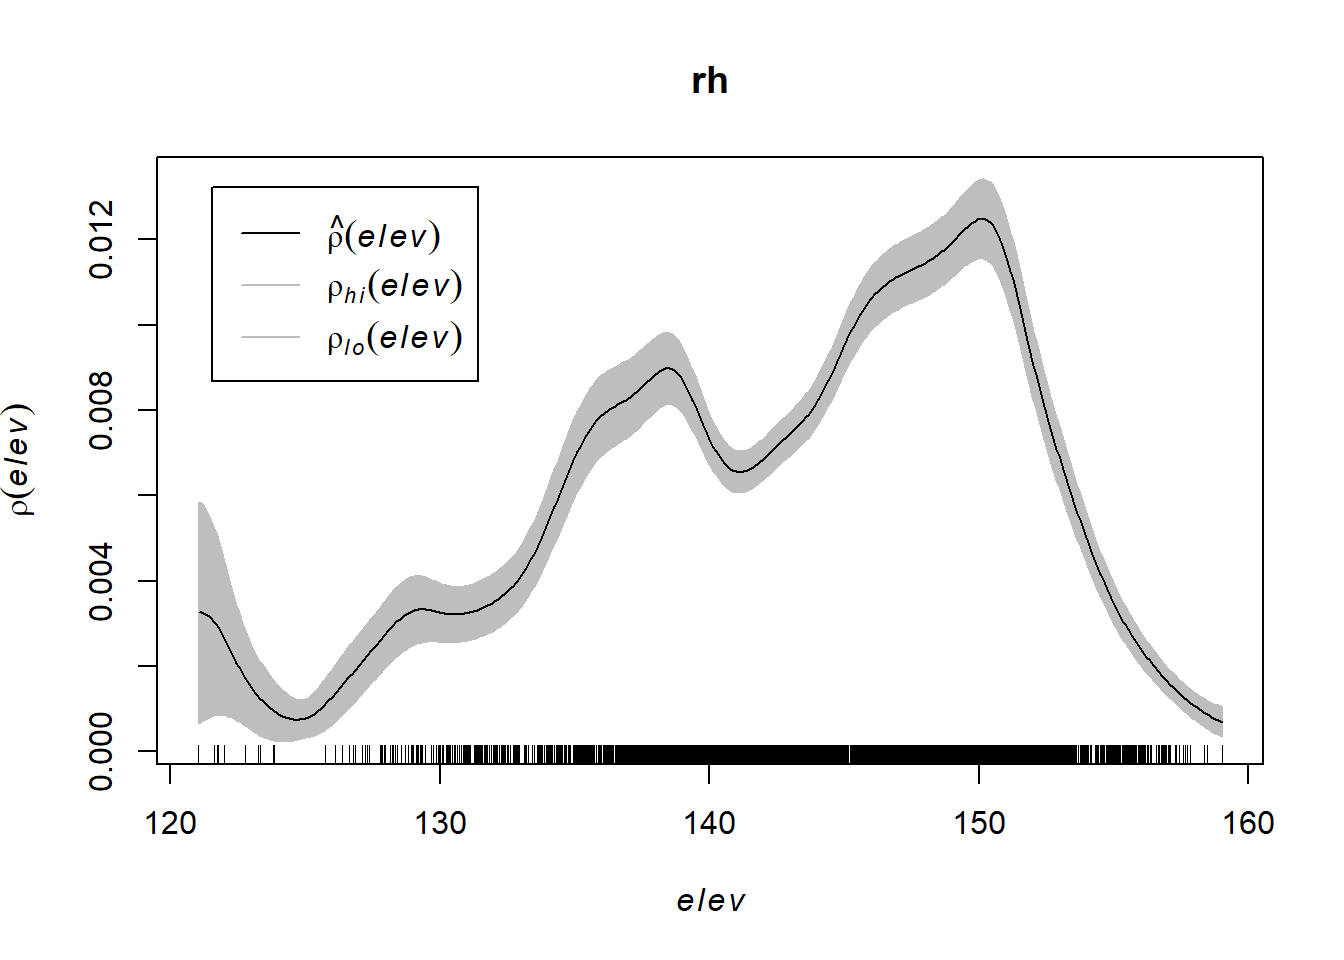
\includegraphics{Applied-Spatial-Data-Analysis_files/figure-latex/unnamed-chunk-32-1.pdf}

Test:

\begin{Shaded}
\begin{Highlighting}[]
\NormalTok{Q3x3test\_cluster }\OtherTok{=} \FunctionTok{quadrat.test}\NormalTok{(pp\_cluster, }\DecValTok{3}\NormalTok{,}\DecValTok{3}\NormalTok{)}
\end{Highlighting}
\end{Shaded}

\begin{verbatim}
## Warning: Some expected counts are small; chi^2 approximation may be inaccurate
\end{verbatim}

\begin{Shaded}
\begin{Highlighting}[]
\NormalTok{Q3x3test\_cluster}
\end{Highlighting}
\end{Shaded}

\begin{verbatim}
## 
##  Chi-squared test of CSR using quadrat counts
## 
## data:  pp_cluster
## X2 = 48.65, df = 8, p-value = 1.484e-07
## alternative hypothesis: two.sided
## 
## Quadrats: 3 by 3 grid of tiles
\end{verbatim}

\hypertarget{simulated-regular-pattern}{%
\subsection{Simulated Regular Pattern}\label{simulated-regular-pattern}}

\begin{Shaded}
\begin{Highlighting}[]
\NormalTok{Q3x3\_regular }\OtherTok{=} \FunctionTok{quadratcount}\NormalTok{(pp\_regular, }\AttributeTok{nx=}\DecValTok{4}\NormalTok{, }\AttributeTok{ny=}\DecValTok{4}\NormalTok{)}
\FunctionTok{plot}\NormalTok{(pp\_regular)}
\FunctionTok{plot}\NormalTok{(Q3x3\_regular, }\AttributeTok{add=}\ConstantTok{TRUE}\NormalTok{, }\AttributeTok{col=}\StringTok{"red"}\NormalTok{, }\AttributeTok{cex=}\FloatTok{1.5}\NormalTok{, }\AttributeTok{lty=}\DecValTok{2}\NormalTok{)}
\end{Highlighting}
\end{Shaded}

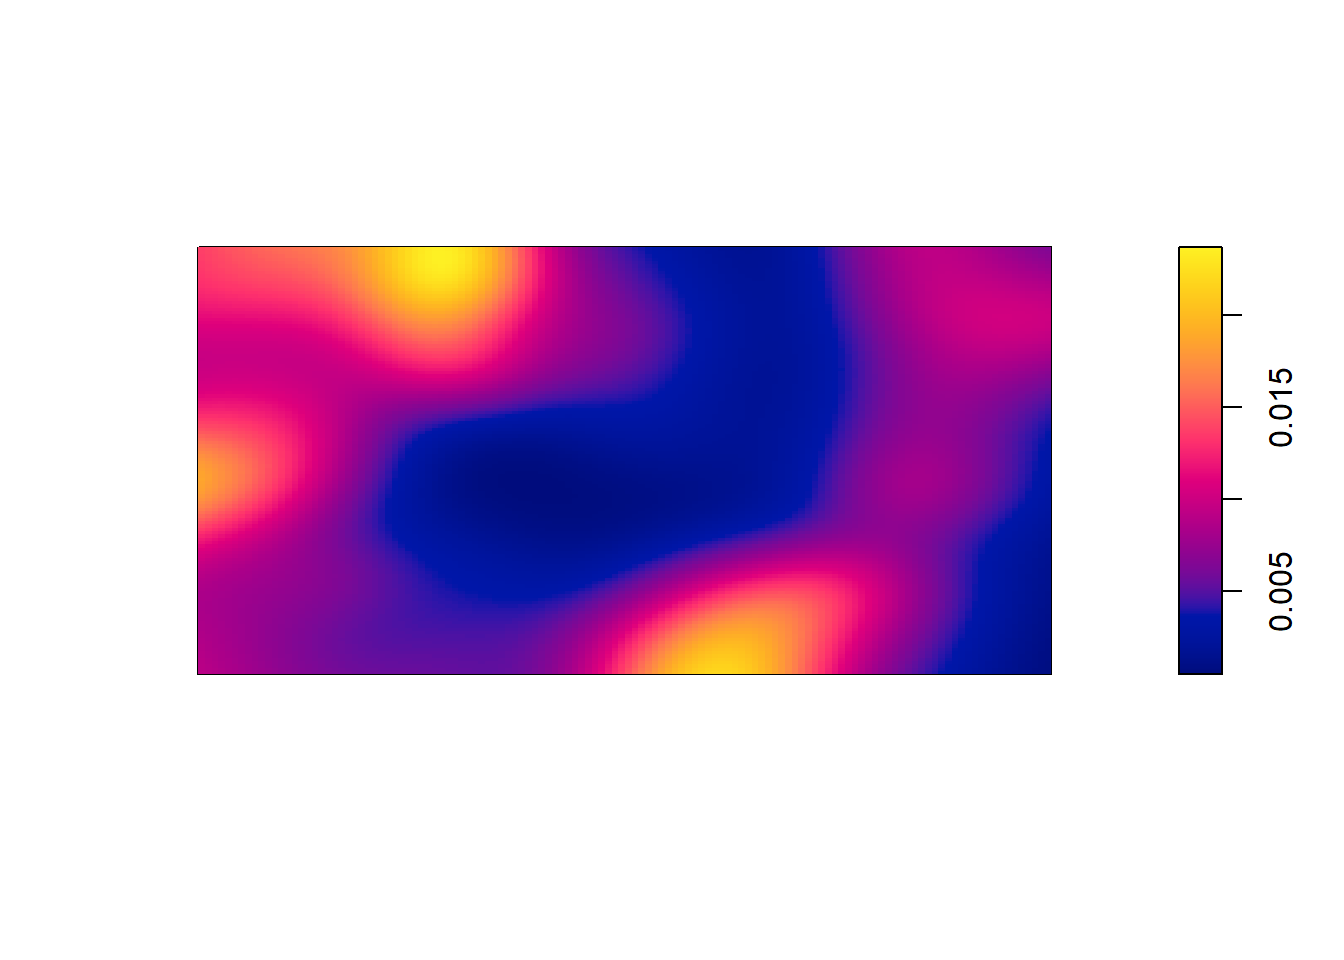
\includegraphics{Applied-Spatial-Data-Analysis_files/figure-latex/unnamed-chunk-34-1.pdf}

Test:

\begin{Shaded}
\begin{Highlighting}[]
\NormalTok{Q3x3test\_regular }\OtherTok{=} \FunctionTok{quadrat.test}\NormalTok{(pp\_regular, }\DecValTok{3}\NormalTok{,}\DecValTok{3}\NormalTok{)}
\end{Highlighting}
\end{Shaded}

\begin{verbatim}
## Warning: Some expected counts are small; chi^2 approximation may be inaccurate
\end{verbatim}

\begin{Shaded}
\begin{Highlighting}[]
\NormalTok{Q3x3test\_regular}
\end{Highlighting}
\end{Shaded}

\begin{verbatim}
## 
##  Chi-squared test of CSR using quadrat counts
## 
## data:  pp_regular
## X2 = 4.55, df = 8, p-value = 0.3912
## alternative hypothesis: two.sided
## 
## Quadrats: 3 by 3 grid of tiles
\end{verbatim}

\hypertarget{kernel-density-smoothing}{%
\section{Kernel Density Smoothing}\label{kernel-density-smoothing}}

\hypertarget{csr-pattern}{%
\subsection{CSR Pattern}\label{csr-pattern}}

\begin{Shaded}
\begin{Highlighting}[]
\NormalTok{den }\OtherTok{\textless{}{-}} \FunctionTok{density}\NormalTok{(pp\_csr, }\AttributeTok{sigma =}\NormalTok{ .}\DecValTok{1}\NormalTok{)}
\FunctionTok{plot}\NormalTok{(den, }\AttributeTok{main =} \StringTok{"CSR"}\NormalTok{)}
\FunctionTok{plot}\NormalTok{(pp\_csr, }\AttributeTok{add=}\ConstantTok{TRUE}\NormalTok{)}
\FunctionTok{contour}\NormalTok{(den, }\AttributeTok{add =} \ConstantTok{TRUE}\NormalTok{)}
\end{Highlighting}
\end{Shaded}

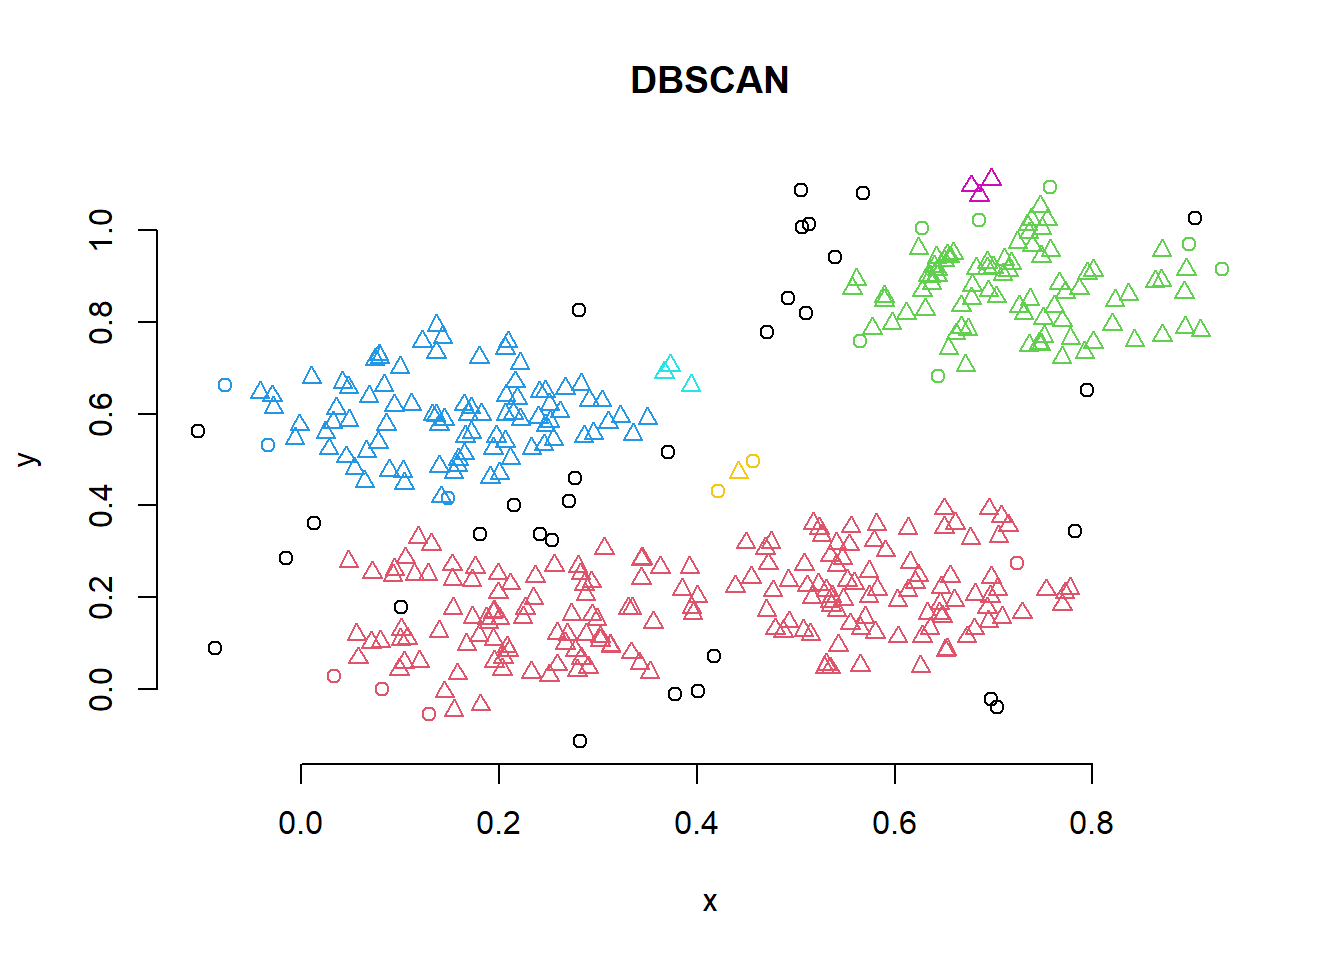
\includegraphics{Applied-Spatial-Data-Analysis_files/figure-latex/unnamed-chunk-36-1.pdf}

\hypertarget{regular-pattern}{%
\subsection{Regular Pattern}\label{regular-pattern}}

\begin{Shaded}
\begin{Highlighting}[]
\NormalTok{den }\OtherTok{\textless{}{-}} \FunctionTok{density}\NormalTok{(pp\_regular)}
\FunctionTok{plot}\NormalTok{(den, }\AttributeTok{main =} \StringTok{"Regular"}\NormalTok{)}
\FunctionTok{plot}\NormalTok{(pp\_regular, }\AttributeTok{add=}\ConstantTok{TRUE}\NormalTok{)}
\FunctionTok{contour}\NormalTok{(den, }\AttributeTok{add=}\ConstantTok{TRUE}\NormalTok{)}
\end{Highlighting}
\end{Shaded}

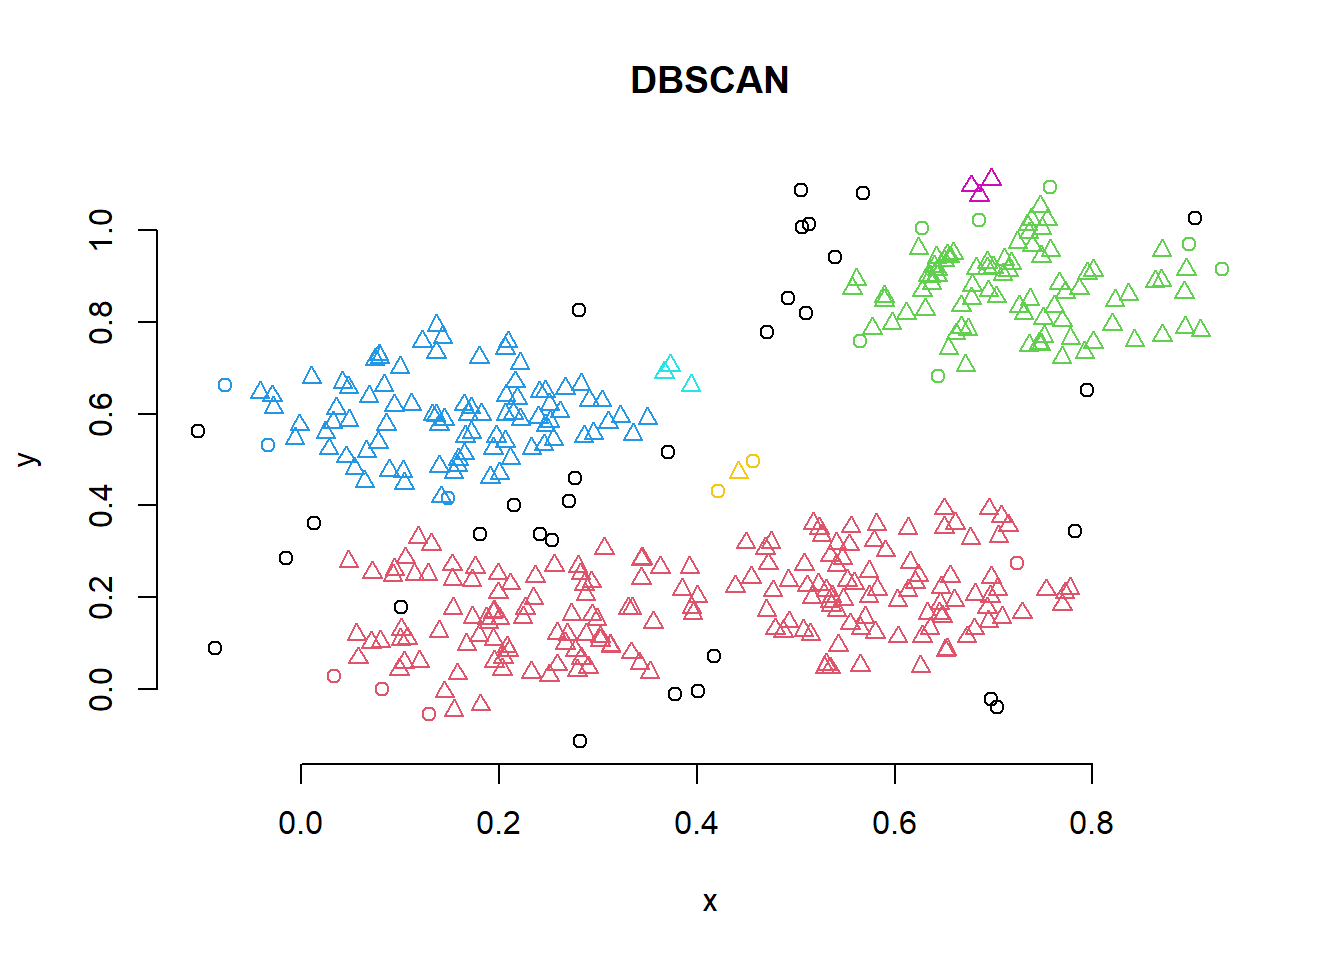
\includegraphics{Applied-Spatial-Data-Analysis_files/figure-latex/unnamed-chunk-37-1.pdf}

\hypertarget{cluster-pattern}{%
\subsection{Cluster Pattern}\label{cluster-pattern}}

\begin{Shaded}
\begin{Highlighting}[]
\NormalTok{den }\OtherTok{\textless{}{-}} \FunctionTok{density}\NormalTok{(pp\_cluster)}
\FunctionTok{plot}\NormalTok{(den, }\AttributeTok{main =} \StringTok{"Cluster"}\NormalTok{)}
\FunctionTok{plot}\NormalTok{(pp\_cluster, }\AttributeTok{add=}\ConstantTok{TRUE}\NormalTok{)}
\FunctionTok{contour}\NormalTok{(den, }\AttributeTok{add=}\ConstantTok{TRUE}\NormalTok{)}
\end{Highlighting}
\end{Shaded}

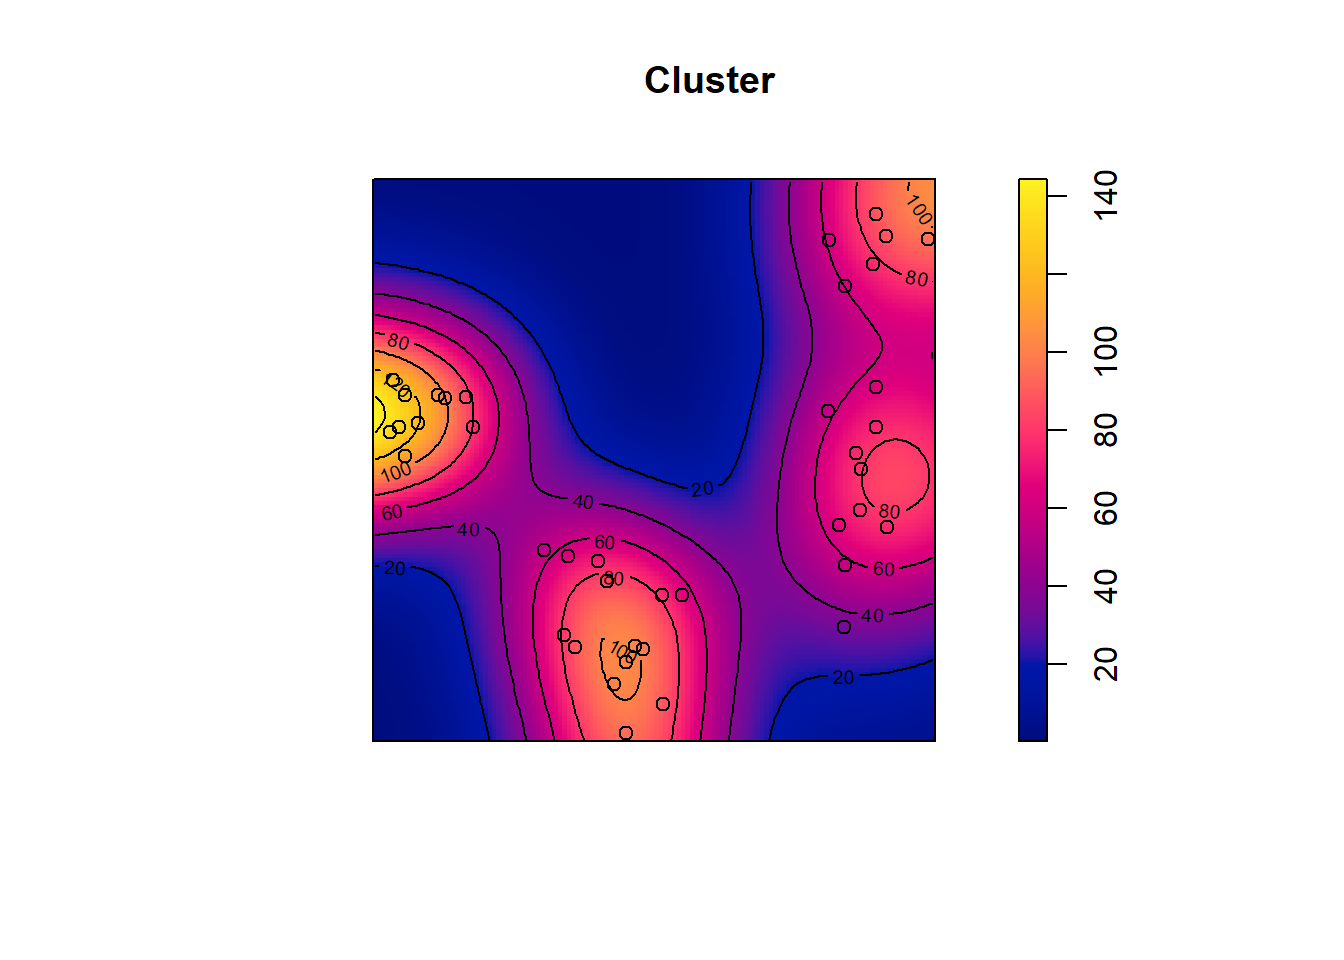
\includegraphics{Applied-Spatial-Data-Analysis_files/figure-latex/unnamed-chunk-38-1.pdf}

\hypertarget{kernel-smoothing-with-a-covariate}{%
\section{Kernel Smoothing with a Covariate}\label{kernel-smoothing-with-a-covariate}}

\hypertarget{tropical-rain-forest-trees-dataset}{%
\subsection{Tropical rain forest trees dataset}\label{tropical-rain-forest-trees-dataset}}

\begin{Shaded}
\begin{Highlighting}[]
\FunctionTok{data}\NormalTok{(}\StringTok{"bei"}\NormalTok{)}
\end{Highlighting}
\end{Shaded}

Assign the elevation covariate to a variable elev by typing

\begin{Shaded}
\begin{Highlighting}[]
\NormalTok{elev }\OtherTok{\textless{}{-}}\NormalTok{ bei.extra}\SpecialCharTok{$}\NormalTok{elev}
\end{Highlighting}
\end{Shaded}

Plot the trees on top of an image of the elevation covariate.

\begin{Shaded}
\begin{Highlighting}[]
\FunctionTok{plot}\NormalTok{(elev, }\AttributeTok{main =} \StringTok{""}\NormalTok{)}
\FunctionTok{plot}\NormalTok{(bei, }\AttributeTok{add =} \ConstantTok{TRUE}\NormalTok{, }\AttributeTok{cex =} \FloatTok{0.3}\NormalTok{, }\AttributeTok{pch =} \DecValTok{16}\NormalTok{, }\AttributeTok{cols =} \StringTok{"white"}\NormalTok{)}
\end{Highlighting}
\end{Shaded}

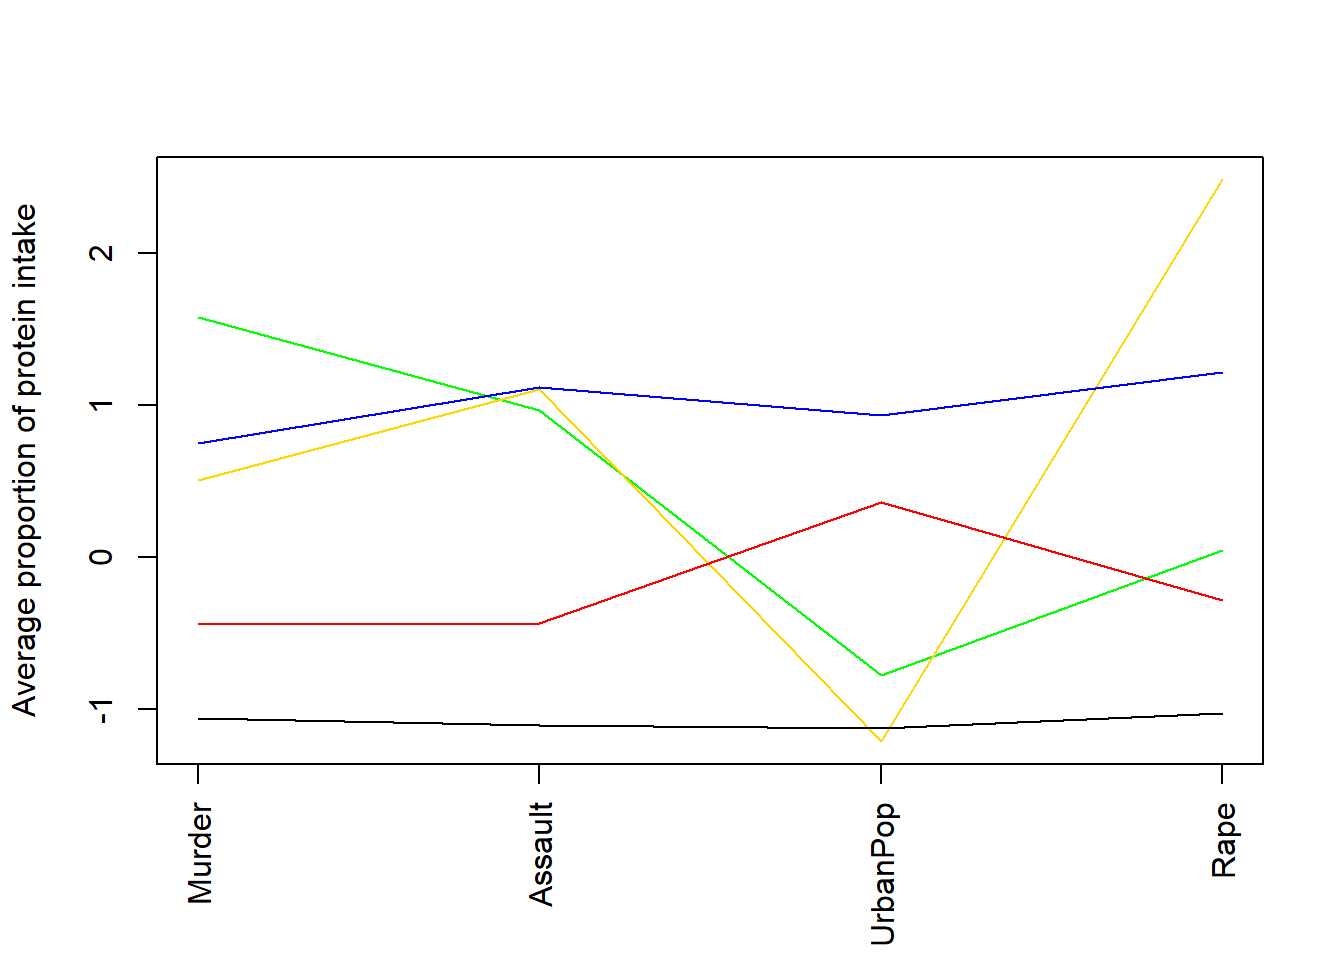
\includegraphics{Applied-Spatial-Data-Analysis_files/figure-latex/unnamed-chunk-41-1.pdf}

For the tropical rainforest data bei, it might be useful to split the study region into several
sub-regions according to the terrain elevation:

\begin{Shaded}
\begin{Highlighting}[]
\NormalTok{b }\OtherTok{\textless{}{-}} \FunctionTok{quantile}\NormalTok{(elev, }\AttributeTok{probs=}\NormalTok{(}\DecValTok{0}\SpecialCharTok{:}\DecValTok{4}\NormalTok{)}\SpecialCharTok{/}\DecValTok{4}\NormalTok{, }\AttributeTok{type=}\DecValTok{2}\NormalTok{)}

\NormalTok{Zcut }\OtherTok{\textless{}{-}} \FunctionTok{cut}\NormalTok{(elev, }\AttributeTok{breaks=}\NormalTok{b, }\AttributeTok{labels=}\FunctionTok{c}\NormalTok{(}\StringTok{"Low"}\NormalTok{, }\StringTok{"Med{-}Low"}\NormalTok{, }\StringTok{"Med{-}High"}\NormalTok{, }\StringTok{"High"}\NormalTok{))}
\FunctionTok{textureplot}\NormalTok{(Zcut, }\AttributeTok{main =} \StringTok{""}\NormalTok{)}
\end{Highlighting}
\end{Shaded}

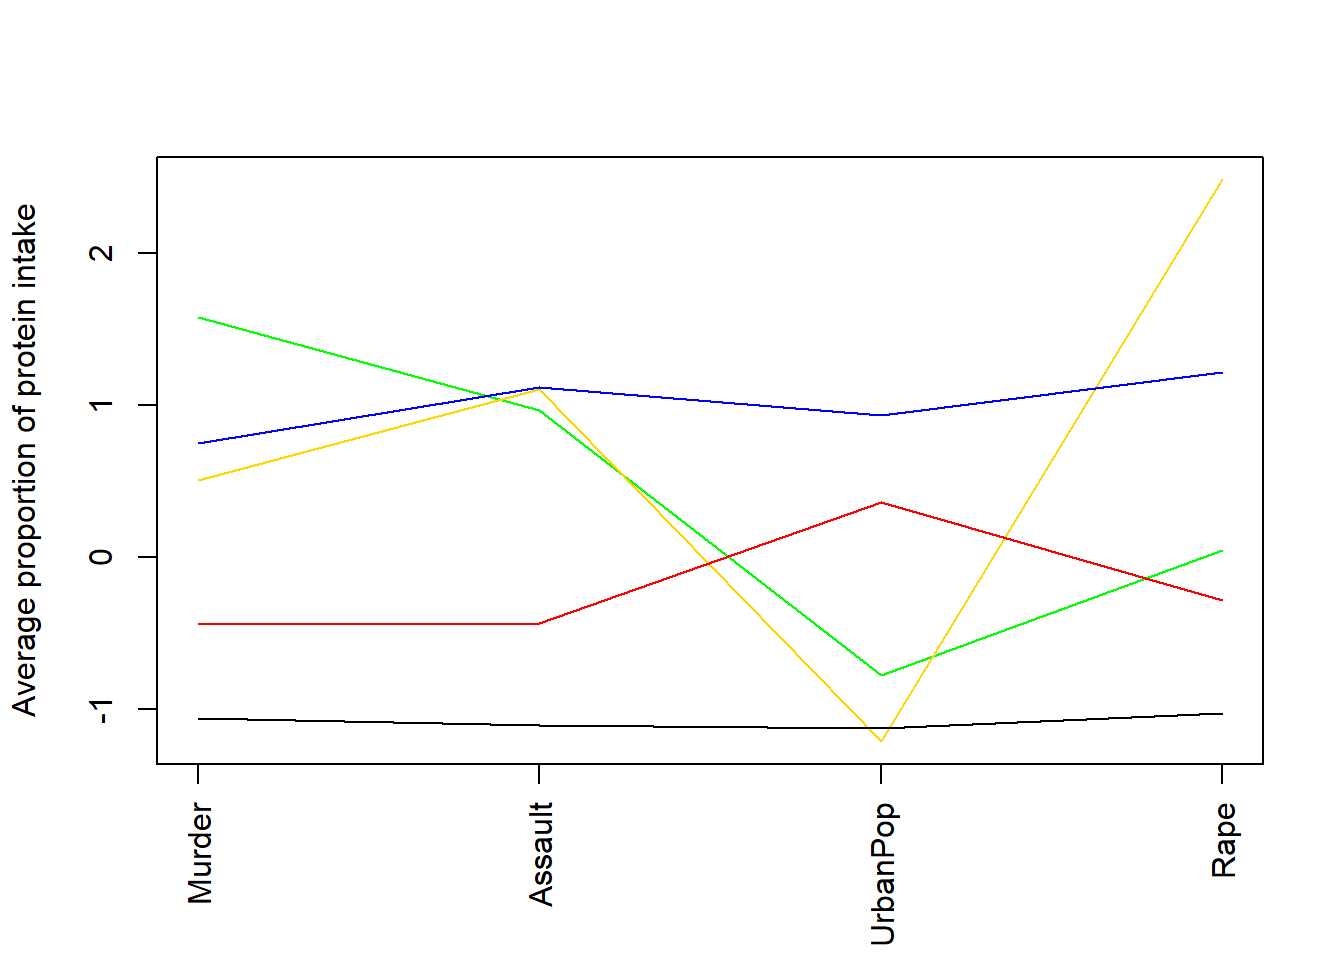
\includegraphics{Applied-Spatial-Data-Analysis_files/figure-latex/unnamed-chunk-42-1.pdf}

Convert the image from above to a tesselation, count the number of points in each region using quadratcount, and plot the quadrat counts.

\begin{Shaded}
\begin{Highlighting}[]
\NormalTok{V }\OtherTok{\textless{}{-}} \FunctionTok{tess}\NormalTok{(}\AttributeTok{image=}\NormalTok{Zcut)}
\NormalTok{qc }\OtherTok{\textless{}{-}} \FunctionTok{quadratcount}\NormalTok{(bei, }\AttributeTok{tess =}\NormalTok{ V)}
\NormalTok{qc}
\end{Highlighting}
\end{Shaded}

\begin{verbatim}
## tile
##      Low  Med-Low Med-High     High 
##      714      883     1344      663
\end{verbatim}

The output shows the number of trees in each region. Since the four regions have equal area, the counts should be approximately equal if there is a uniform density of trees. Obviously they are not equal; there appears to be a strong preference for higher elevations (dropping off for the highest elevations).

Estimate the intensity in each of the four regions.

\begin{Shaded}
\begin{Highlighting}[]
\FunctionTok{intensity}\NormalTok{(qc)}
\end{Highlighting}
\end{Shaded}

\begin{verbatim}
## tile
##         Low     Med-Low    Med-High        High 
## 0.005623154 0.006960978 0.010593103 0.005228707
\end{verbatim}

Assume that the intensity of trees is a function (\lambda(u) = \rho(e(u))) where (e(u)) is the terrain elevation at location u.

Compute a nonparametric estimate of the function (\rho) and plot it by

\begin{Shaded}
\begin{Highlighting}[]
\NormalTok{rh }\OtherTok{\textless{}{-}} \FunctionTok{rhohat}\NormalTok{(bei, elev)}
\FunctionTok{plot}\NormalTok{(rh)}
\end{Highlighting}
\end{Shaded}

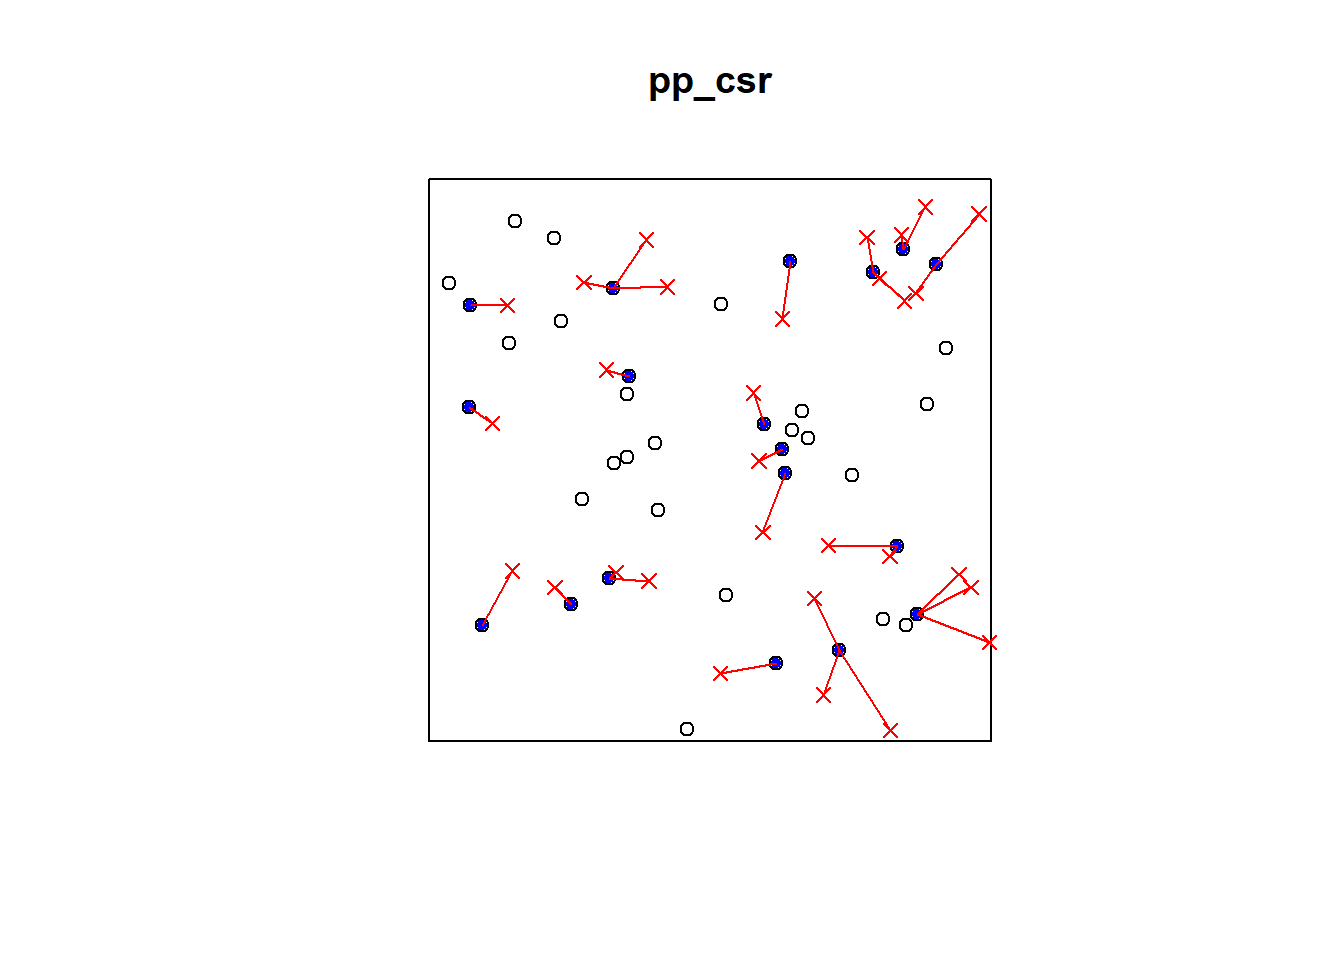
\includegraphics{Applied-Spatial-Data-Analysis_files/figure-latex/unnamed-chunk-45-1.pdf}

Compute the predicted intensity based on this estimate of (\rho).

\begin{Shaded}
\begin{Highlighting}[]
\NormalTok{predictedrho }\OtherTok{\textless{}{-}} \FunctionTok{predict}\NormalTok{(rh)}
\FunctionTok{plot}\NormalTok{(predictedrho, }\AttributeTok{main =} \StringTok{""}\NormalTok{)}
\FunctionTok{plot}\NormalTok{(bei, }\AttributeTok{add =} \ConstantTok{TRUE}\NormalTok{, }\AttributeTok{cols =} \StringTok{"white"}\NormalTok{, }\AttributeTok{cex =}\NormalTok{ .}\DecValTok{2}\NormalTok{, }\AttributeTok{pch =} \DecValTok{16}\NormalTok{)}
\end{Highlighting}
\end{Shaded}

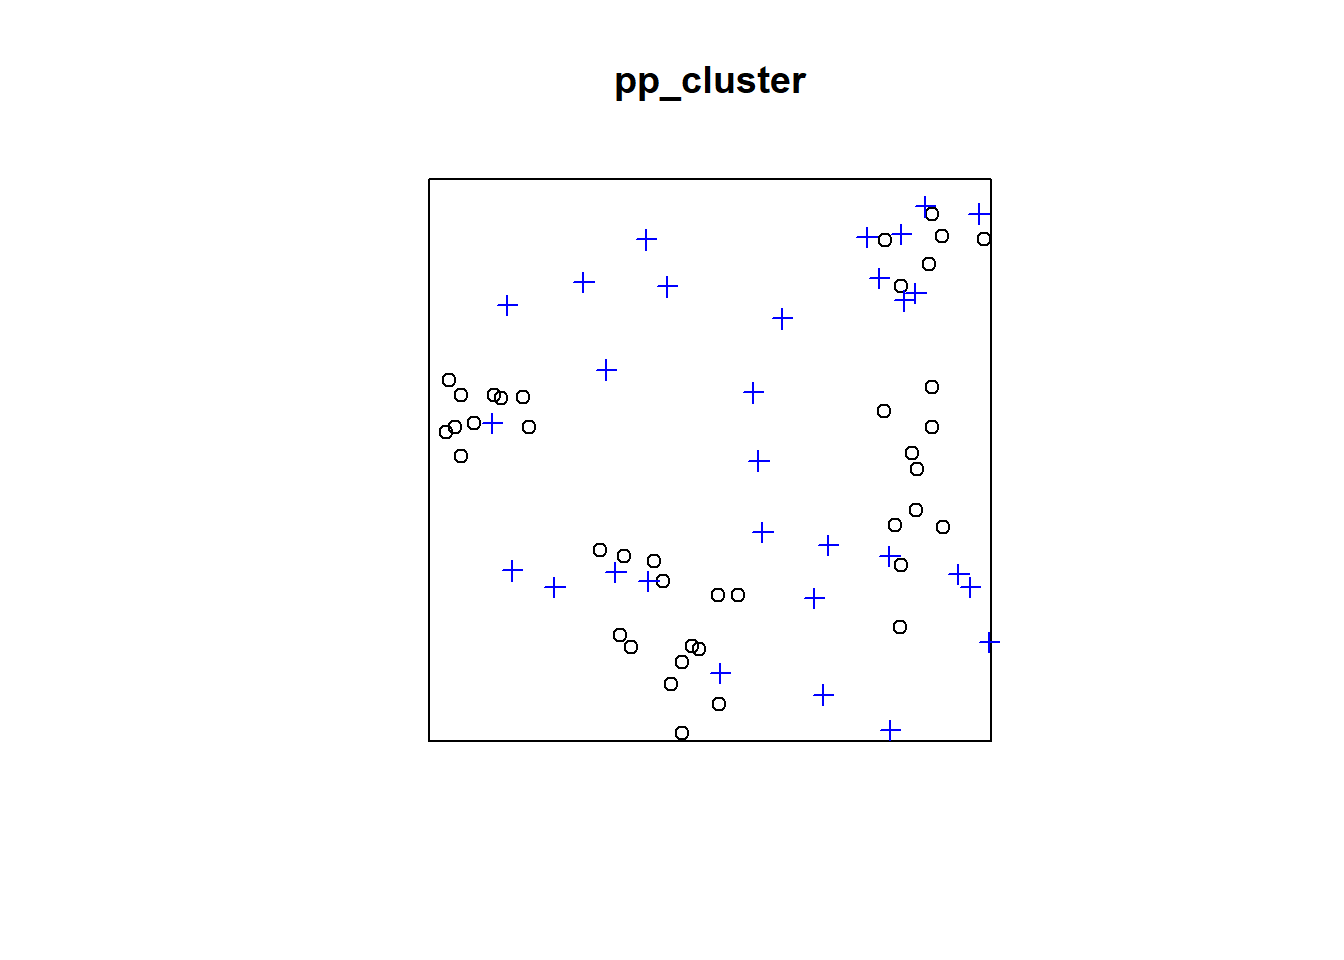
\includegraphics{Applied-Spatial-Data-Analysis_files/figure-latex/unnamed-chunk-46-1.pdf}

Compute a non-parametric estimate by kernel smoothing and compare with the predicted intensity above.

The kernel density estimate of the points is computed and plotted with the following code:

\begin{Shaded}
\begin{Highlighting}[]
\NormalTok{kerneldensity }\OtherTok{\textless{}{-}} \FunctionTok{density}\NormalTok{(bei, }\AttributeTok{sigma =}\NormalTok{ bw.scott)}
\FunctionTok{plot}\NormalTok{(kerneldensity, }\AttributeTok{main =} \StringTok{""}\NormalTok{)}
\FunctionTok{plot}\NormalTok{(kerneldensity, }\AttributeTok{add =} \ConstantTok{TRUE}\NormalTok{, }\AttributeTok{cols =} \StringTok{"white"}\NormalTok{, }\AttributeTok{cex =}\NormalTok{ .}\DecValTok{2}\NormalTok{, }\AttributeTok{pch =} \DecValTok{16}\NormalTok{)}
\end{Highlighting}
\end{Shaded}

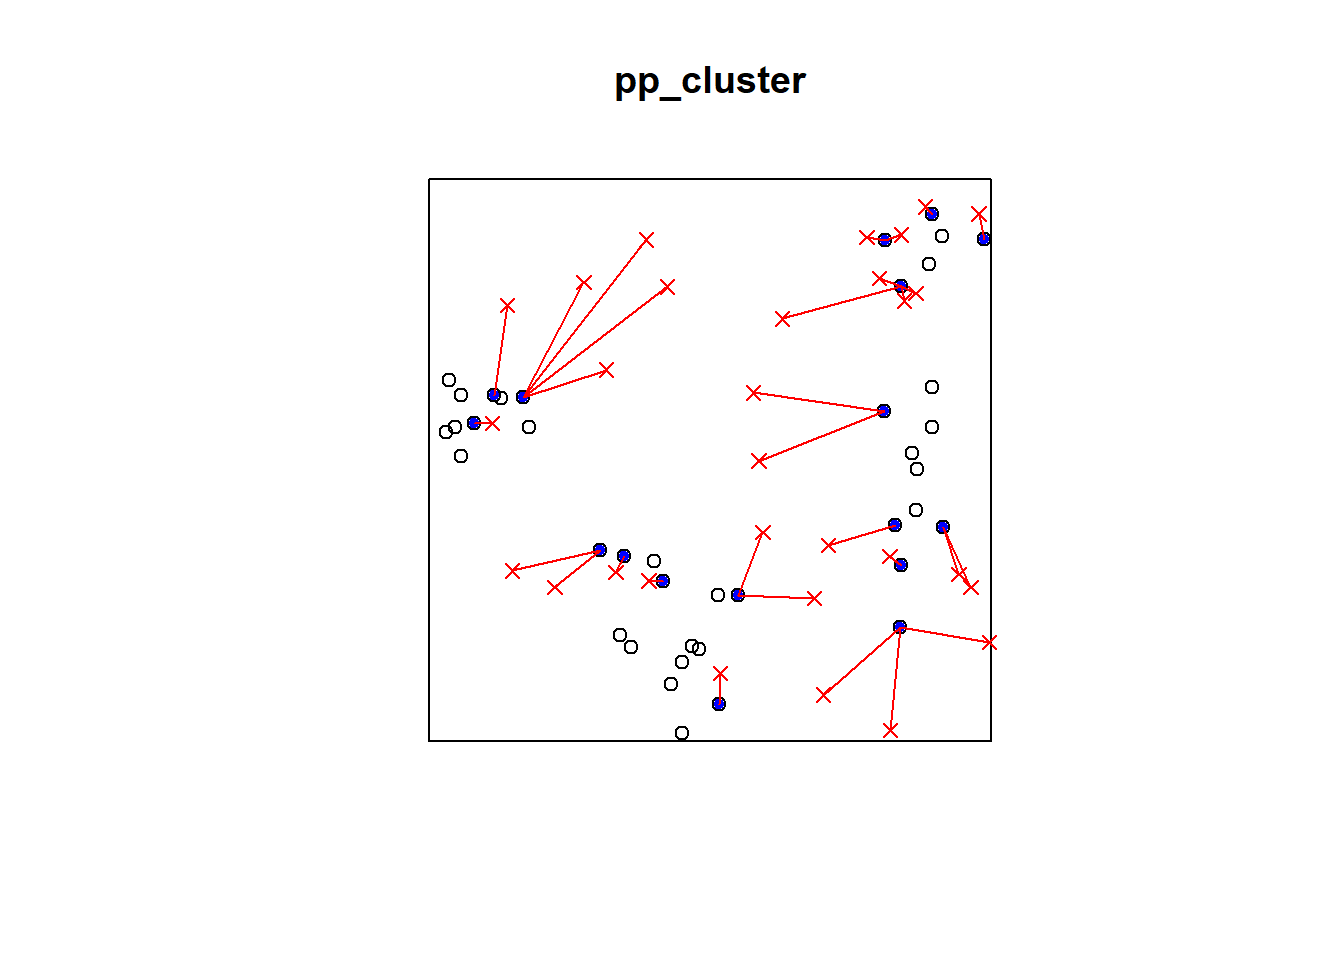
\includegraphics{Applied-Spatial-Data-Analysis_files/figure-latex/unnamed-chunk-47-1.pdf}

Compare the two

\begin{Shaded}
\begin{Highlighting}[]
\FunctionTok{pairs}\NormalTok{(predictedrho, kerneldensity)}
\end{Highlighting}
\end{Shaded}

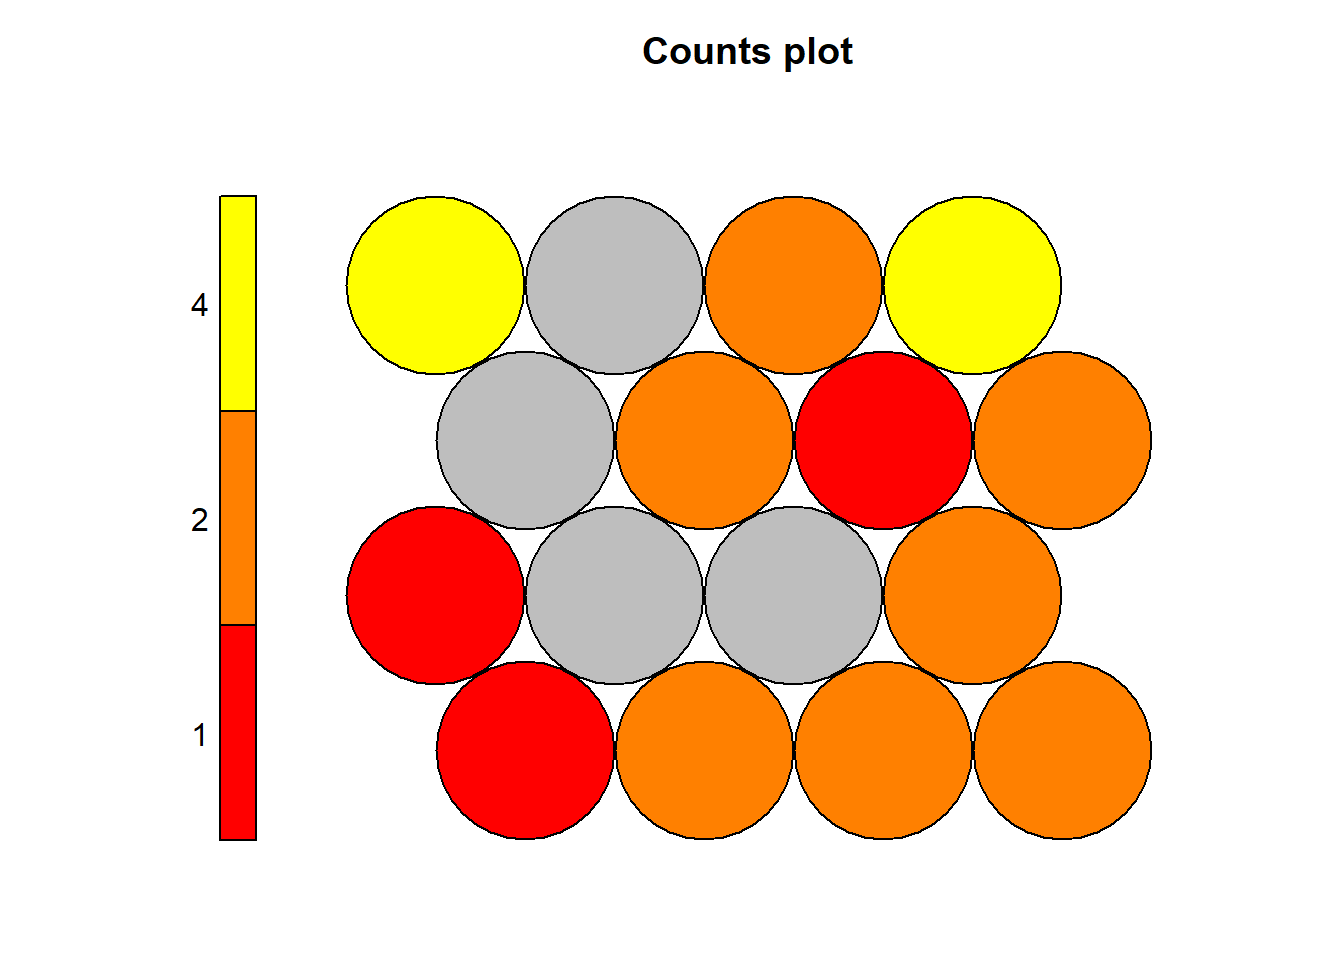
\includegraphics{Applied-Spatial-Data-Analysis_files/figure-latex/unnamed-chunk-48-1.pdf}

\begin{Shaded}
\begin{Highlighting}[]
\FunctionTok{plot}\NormalTok{(}\FunctionTok{eval.im}\NormalTok{(kerneldensity}\SpecialCharTok{{-}}\NormalTok{predictedrho))}
\end{Highlighting}
\end{Shaded}

\begin{verbatim}
## Warning: the images 'kerneldensity' and 'predictedrho' were not compatible
\end{verbatim}

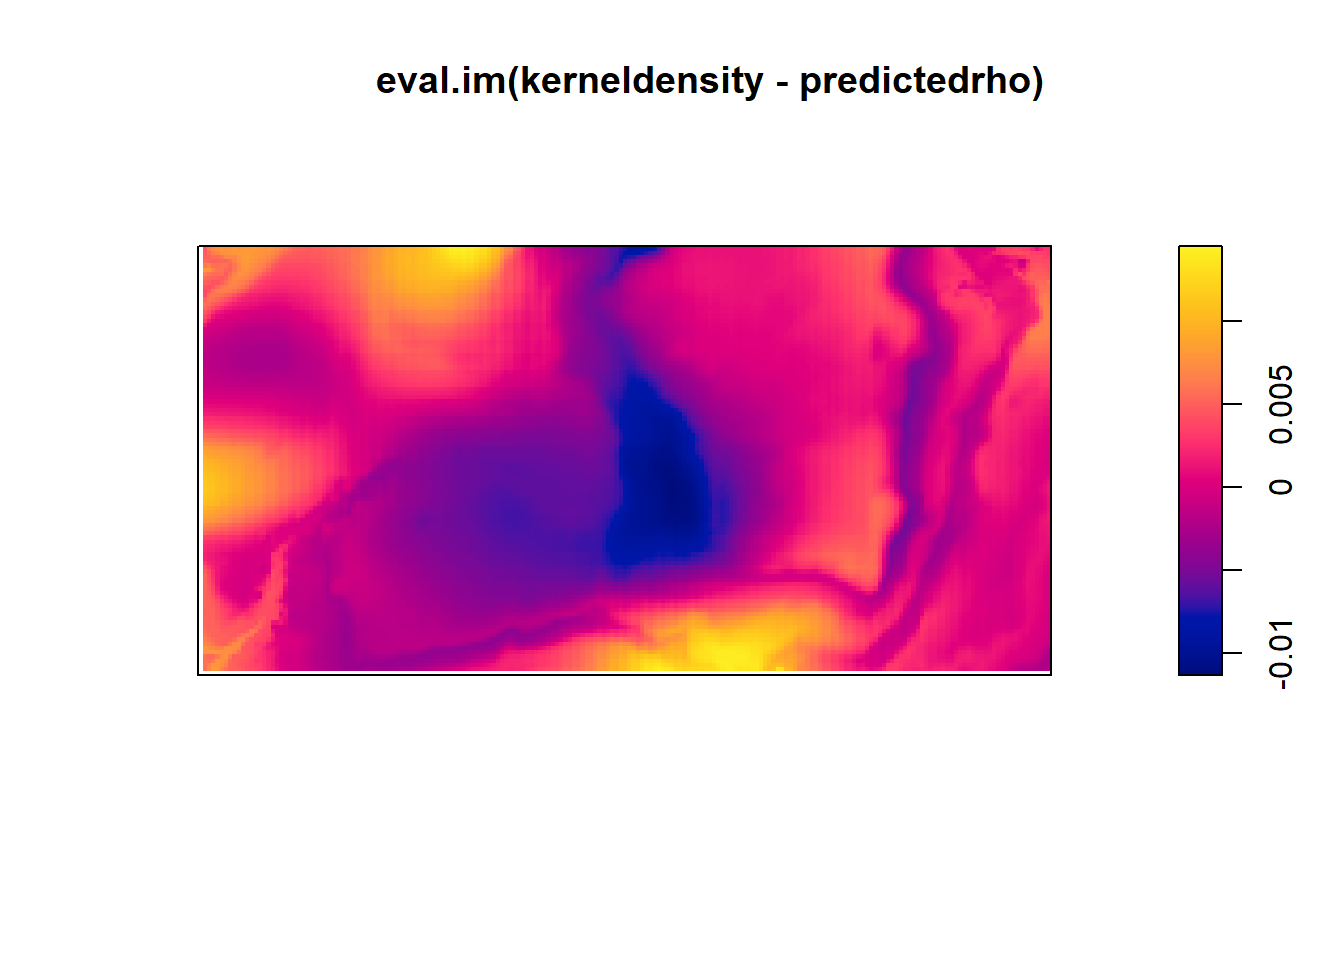
\includegraphics{Applied-Spatial-Data-Analysis_files/figure-latex/unnamed-chunk-48-2.pdf}

Which seems to be quite different form the predicted intensity.

\hypertarget{distance-measures-and-tests}{%
\section{Distance Measures and Tests}\label{distance-measures-and-tests}}

\hypertarget{e2e-distances}{%
\subsection{e2e Distances}\label{e2e-distances}}

\hypertarget{swp-dataset-1}{%
\subsubsection{swp dataset}\label{swp-dataset-1}}

\begin{Shaded}
\begin{Highlighting}[]
\NormalTok{PD }\OtherTok{=} \FunctionTok{pairdist}\NormalTok{(swp)}
\FunctionTok{class}\NormalTok{(PD)}
\end{Highlighting}
\end{Shaded}

\begin{verbatim}
## [1] "matrix" "array"
\end{verbatim}

\begin{Shaded}
\begin{Highlighting}[]
\NormalTok{dm }\OtherTok{\textless{}{-}} \FunctionTok{as.matrix}\NormalTok{(PD)}
\NormalTok{dm[}\DecValTok{1}\SpecialCharTok{:}\DecValTok{5}\NormalTok{, }\DecValTok{1}\SpecialCharTok{:}\DecValTok{5}\NormalTok{]}
\end{Highlighting}
\end{Shaded}

\begin{verbatim}
##          [,1]     [,2]     [,3]     [,4]     [,5]
## [1,] 0.000000 2.700000 3.701351 1.503330 5.433231
## [2,] 2.700000 0.000000 1.004988 1.204159 2.765863
## [3,] 3.701351 1.004988 0.000000 2.200000 1.772005
## [4,] 1.503330 1.204159 2.200000 0.000000 3.931921
## [5,] 5.433231 2.765863 1.772005 3.931921 0.000000
\end{verbatim}

\begin{Shaded}
\begin{Highlighting}[]
\FunctionTok{diag}\NormalTok{(dm) }\OtherTok{\textless{}{-}} \ConstantTok{NA}
\CommentTok{\#dm[1:5, 1:5]}
\NormalTok{wdmin }\OtherTok{\textless{}{-}} \FunctionTok{apply}\NormalTok{(dm, }\DecValTok{1}\NormalTok{, which.min)}

\NormalTok{dmin }\OtherTok{\textless{}{-}} \FunctionTok{apply}\NormalTok{(dm, }\DecValTok{1}\NormalTok{, min, }\AttributeTok{na.rm=}\ConstantTok{TRUE}\NormalTok{)}
\FunctionTok{head}\NormalTok{(dmin)}
\end{Highlighting}
\end{Shaded}

\begin{verbatim}
## [1] 1.5033296 0.8544004 1.0049876 0.9055385 1.0770330 0.8544004
\end{verbatim}

\begin{Shaded}
\begin{Highlighting}[]
\CommentTok{\# which is the same as nndist e2e=nndist(swp)}

\NormalTok{dmin }\OtherTok{=} \FunctionTok{nndist}\NormalTok{(swp)}

\FunctionTok{plot}\NormalTok{(swp)}
\NormalTok{xy }\OtherTok{=} \FunctionTok{cbind}\NormalTok{(swp}\SpecialCharTok{$}\NormalTok{x, swp}\SpecialCharTok{$}\NormalTok{y)}

\NormalTok{ord }\OtherTok{\textless{}{-}} \FunctionTok{rev}\NormalTok{(}\FunctionTok{order}\NormalTok{(dmin))}
\NormalTok{far25 }\OtherTok{\textless{}{-}}\NormalTok{ ord[}\DecValTok{1}\SpecialCharTok{:}\DecValTok{71}\NormalTok{]}
\NormalTok{neighbors }\OtherTok{\textless{}{-}}\NormalTok{ wdmin[far25]}
\FunctionTok{points}\NormalTok{(xy[far25, ], }\AttributeTok{col=}\StringTok{\textquotesingle{}blue\textquotesingle{}}\NormalTok{, }\AttributeTok{pch=}\DecValTok{20}\NormalTok{)}
\FunctionTok{points}\NormalTok{(xy[neighbors, ], }\AttributeTok{col=}\StringTok{\textquotesingle{}red\textquotesingle{}}\NormalTok{)}
\CommentTok{\# drawing the lines, easiest via a loop}
\ControlFlowTok{for}\NormalTok{ (i }\ControlFlowTok{in}\NormalTok{ far25) \{}
    \FunctionTok{lines}\NormalTok{(}\FunctionTok{rbind}\NormalTok{(xy[i, ], xy[wdmin[i], ]), }\AttributeTok{col=}\StringTok{\textquotesingle{}red\textquotesingle{}}\NormalTok{)}
\NormalTok{\}}
\end{Highlighting}
\end{Shaded}

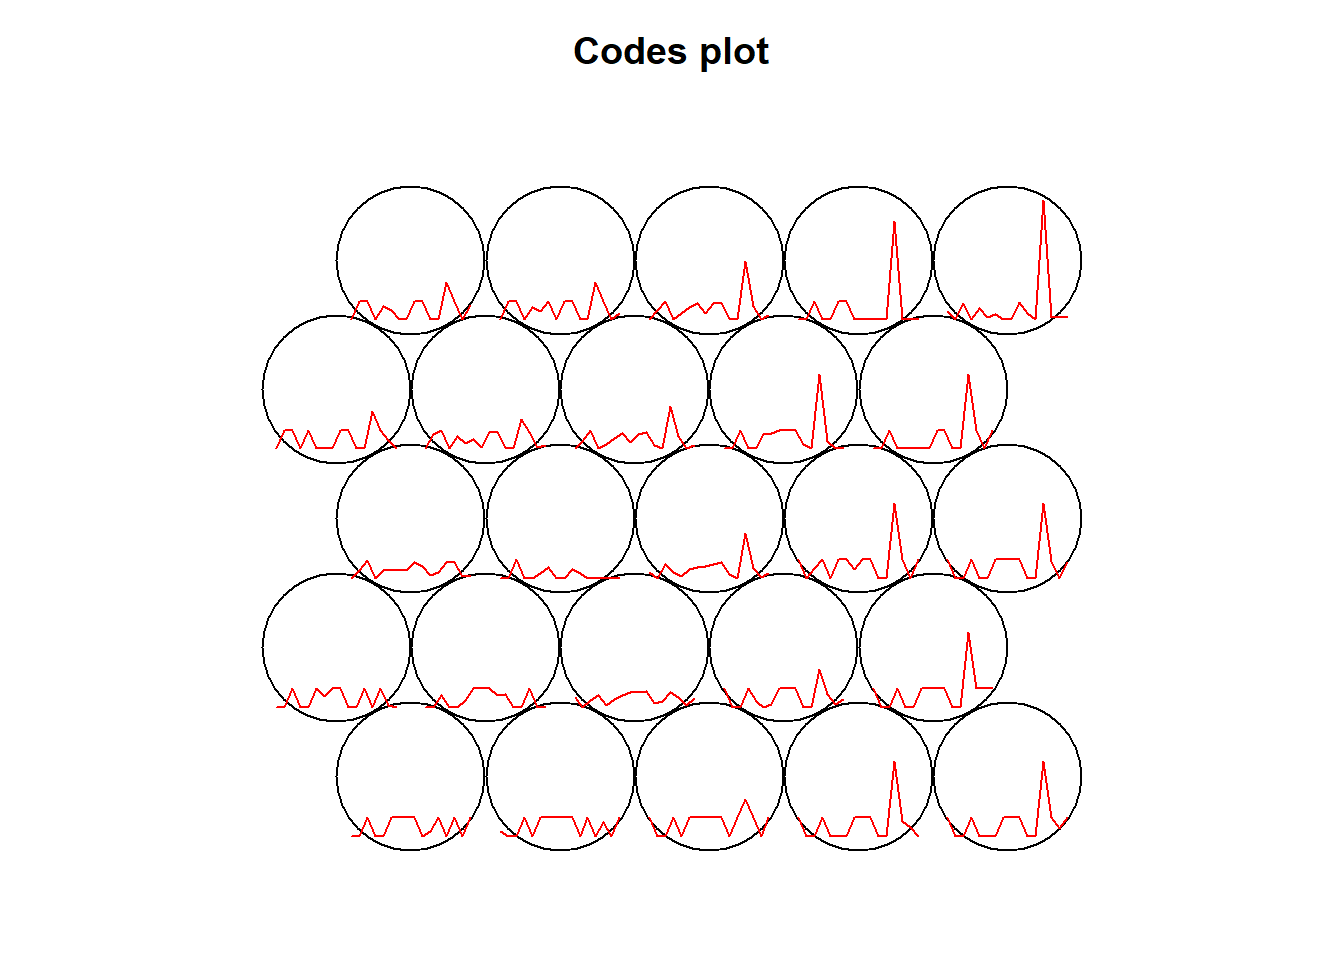
\includegraphics{Applied-Spatial-Data-Analysis_files/figure-latex/unnamed-chunk-49-1.pdf}

\hypertarget{simulated-csr-pattern-1}{%
\subsubsection{Simulated CSR Pattern}\label{simulated-csr-pattern-1}}

\begin{Shaded}
\begin{Highlighting}[]
\NormalTok{e2e\_csr }\OtherTok{=} \FunctionTok{nndist}\NormalTok{(pp\_csr)}
\NormalTok{e2e\_csr}
\end{Highlighting}
\end{Shaded}

\begin{verbatim}
##  [1] 0.11056220 0.05419105 0.08163249 0.05574520 0.19907565 0.03191166
##  [7] 0.10456756 0.15049858 0.16325765 0.02841510 0.05044346 0.05419105
## [13] 0.10456756 0.07525211 0.02471890 0.08651227 0.03700818 0.06471165
## [19] 0.12663659 0.08163249 0.06471165 0.07525211 0.14362670 0.03195288
## [25] 0.09669706 0.03195288 0.09731910 0.04284774 0.11297958 0.03191166
## [31] 0.13454666 0.02841510 0.02471890 0.06711512 0.10924574 0.04269836
## [37] 0.09947882 0.03815278 0.14362670 0.10235020
\end{verbatim}

\begin{Shaded}
\begin{Highlighting}[]
\NormalTok{PD }\OtherTok{=} \FunctionTok{pairdist}\NormalTok{(pp\_csr)}
\FunctionTok{class}\NormalTok{(PD)}
\end{Highlighting}
\end{Shaded}

\begin{verbatim}
## [1] "matrix" "array"
\end{verbatim}

\begin{Shaded}
\begin{Highlighting}[]
\NormalTok{dm }\OtherTok{\textless{}{-}} \FunctionTok{as.matrix}\NormalTok{(PD)}
\NormalTok{dm[}\DecValTok{1}\SpecialCharTok{:}\DecValTok{5}\NormalTok{, }\DecValTok{1}\SpecialCharTok{:}\DecValTok{5}\NormalTok{]}
\end{Highlighting}
\end{Shaded}

\begin{verbatim}
##           [,1]      [,2]      [,3]      [,4]      [,5]
## [1,] 0.0000000 0.2930205 0.5163115 0.2844957 0.7955061
## [2,] 0.2930205 0.0000000 0.5975953 0.4633681 0.8993362
## [3,] 0.5163115 0.5975953 0.0000000 0.2546708 0.3017974
## [4,] 0.2844957 0.4633681 0.2546708 0.0000000 0.5130861
## [5,] 0.7955061 0.8993362 0.3017974 0.5130861 0.0000000
\end{verbatim}

\begin{Shaded}
\begin{Highlighting}[]
\FunctionTok{diag}\NormalTok{(dm) }\OtherTok{\textless{}{-}} \ConstantTok{NA}
\CommentTok{\#dm[1:5, 1:5]}
\NormalTok{wdmin }\OtherTok{\textless{}{-}} \FunctionTok{apply}\NormalTok{(dm, }\DecValTok{1}\NormalTok{, which.min)}

\NormalTok{dmin }\OtherTok{\textless{}{-}} \FunctionTok{apply}\NormalTok{(dm, }\DecValTok{1}\NormalTok{, min, }\AttributeTok{na.rm=}\ConstantTok{TRUE}\NormalTok{)}
\FunctionTok{head}\NormalTok{(dmin)}
\end{Highlighting}
\end{Shaded}

\begin{verbatim}
## [1] 0.11056220 0.05419105 0.08163249 0.05574520 0.19907565 0.03191166
\end{verbatim}

\begin{Shaded}
\begin{Highlighting}[]
\CommentTok{\# which is the same as nndist e2e=nndist(swp)}

\NormalTok{dmin }\OtherTok{=} \FunctionTok{nndist}\NormalTok{(pp\_csr)}

\FunctionTok{plot}\NormalTok{(pp\_csr)}
\NormalTok{xy }\OtherTok{=} \FunctionTok{cbind}\NormalTok{(pp\_csr}\SpecialCharTok{$}\NormalTok{x, pp\_csr}\SpecialCharTok{$}\NormalTok{y)}

\NormalTok{ord }\OtherTok{\textless{}{-}} \FunctionTok{rev}\NormalTok{(}\FunctionTok{order}\NormalTok{(dmin))}
\NormalTok{far25 }\OtherTok{\textless{}{-}}\NormalTok{ ord[}\DecValTok{1}\SpecialCharTok{:}\DecValTok{40}\NormalTok{]}
\NormalTok{neighbors }\OtherTok{\textless{}{-}}\NormalTok{ wdmin[far25]}
\FunctionTok{points}\NormalTok{(xy[far25, ], }\AttributeTok{col=}\StringTok{\textquotesingle{}blue\textquotesingle{}}\NormalTok{, }\AttributeTok{pch=}\DecValTok{20}\NormalTok{)}
\FunctionTok{points}\NormalTok{(xy[neighbors, ], }\AttributeTok{col=}\StringTok{\textquotesingle{}red\textquotesingle{}}\NormalTok{)}
\CommentTok{\# drawing the lines, easiest via a loop}
\ControlFlowTok{for}\NormalTok{ (i }\ControlFlowTok{in}\NormalTok{ far25) \{}
    \FunctionTok{lines}\NormalTok{(}\FunctionTok{rbind}\NormalTok{(xy[i, ], xy[wdmin[i], ]), }\AttributeTok{col=}\StringTok{\textquotesingle{}red\textquotesingle{}}\NormalTok{)}
\NormalTok{\}}
\end{Highlighting}
\end{Shaded}

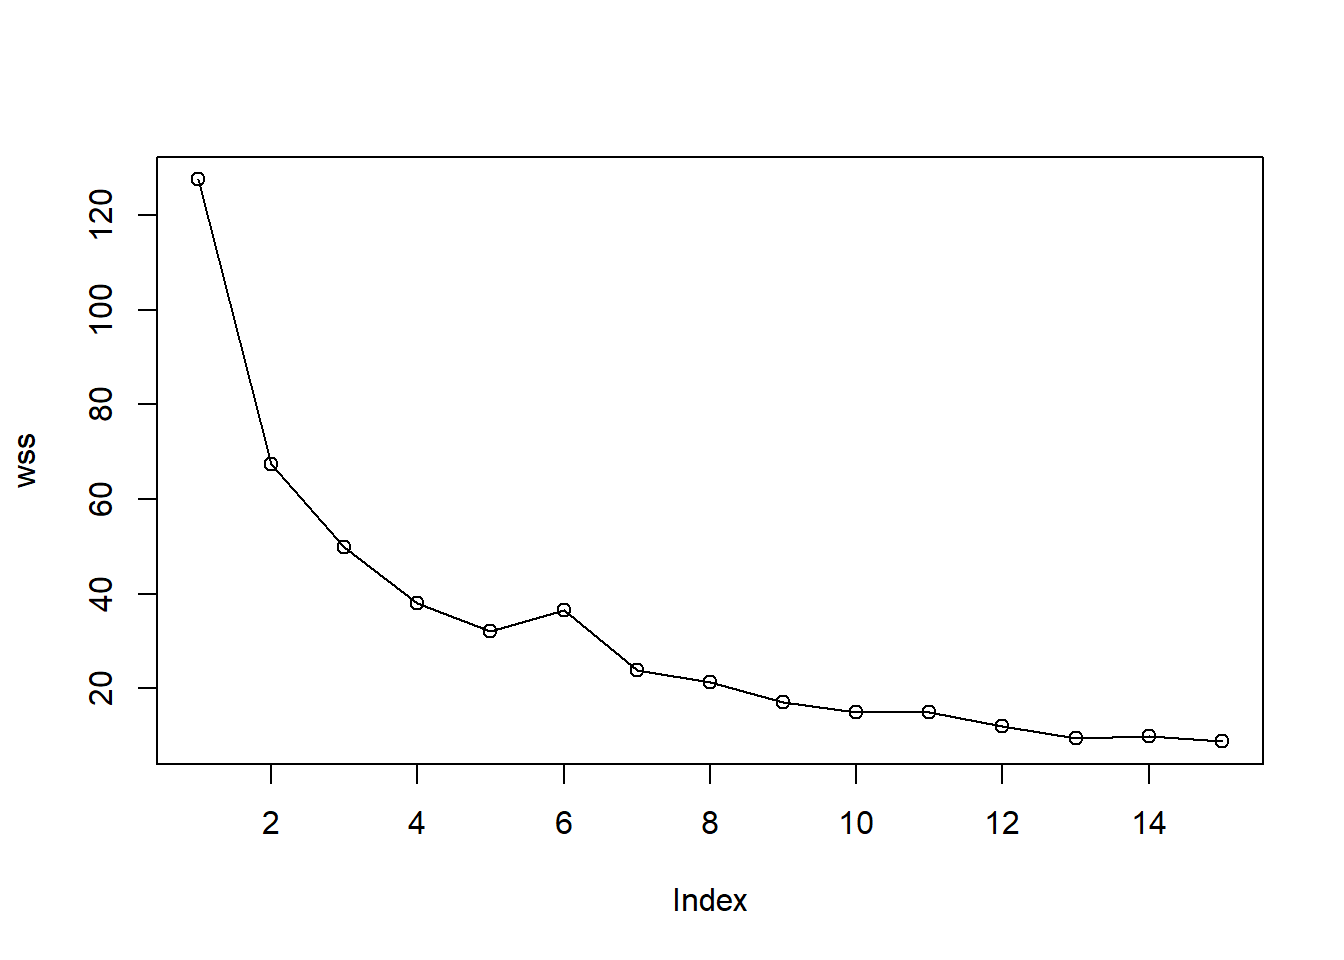
\includegraphics{Applied-Spatial-Data-Analysis_files/figure-latex/unnamed-chunk-51-1.pdf}

\hypertarget{simulated-cluster-pattern-1}{%
\subsubsection{Simulated Cluster Pattern}\label{simulated-cluster-pattern-1}}

\begin{Shaded}
\begin{Highlighting}[]
\NormalTok{e2e\_cluster }\OtherTok{=} \FunctionTok{nndist}\NormalTok{(pp\_cluster)}
\NormalTok{e2e\_cluster}
\end{Highlighting}
\end{Shaded}

\begin{verbatim}
##  [1] 0.01854666 0.03502091 0.01854666 0.04969353 0.03502091 0.03390187
##  [7] 0.01268286 0.05624330 0.01268286 0.03830134 0.04275255 0.02983313
## [13] 0.04275255 0.02983313 0.03774271 0.03774271 0.03391843 0.01376367
## [19] 0.01376367 0.03500058 0.08344093 0.06403124 0.05422191 0.08344093
## [25] 0.03500058 0.08988091 0.04304986 0.07202173 0.04586212 0.02906394
## [31] 0.08760076 0.11053898 0.04586212 0.02906394 0.05896243 0.07149045
## [37] 0.04361429 0.04361429 0.05745563 0.07483198
\end{verbatim}

\begin{Shaded}
\begin{Highlighting}[]
\NormalTok{PD\_cluster }\OtherTok{=} \FunctionTok{pairdist}\NormalTok{(pp\_cluster)}
\FunctionTok{class}\NormalTok{(PD\_cluster)}
\end{Highlighting}
\end{Shaded}

\begin{verbatim}
## [1] "matrix" "array"
\end{verbatim}

\begin{Shaded}
\begin{Highlighting}[]
\NormalTok{dm\_cluster }\OtherTok{\textless{}{-}} \FunctionTok{as.matrix}\NormalTok{(PD\_cluster)}
\NormalTok{dm\_cluster[}\DecValTok{1}\SpecialCharTok{:}\DecValTok{5}\NormalTok{, }\DecValTok{1}\SpecialCharTok{:}\DecValTok{5}\NormalTok{]}
\end{Highlighting}
\end{Shaded}

\begin{verbatim}
##            [,1]       [,2]       [,3]       [,4]       [,5]
## [1,] 0.00000000 0.09345138 0.01854666 0.04969353 0.07093497
## [2,] 0.09345138 0.00000000 0.08597921 0.13688899 0.03502091
## [3,] 0.01854666 0.08597921 0.00000000 0.05097721 0.05847323
## [4,] 0.04969353 0.13688899 0.05097721 0.00000000 0.10757315
## [5,] 0.07093497 0.03502091 0.05847323 0.10757315 0.00000000
\end{verbatim}

\begin{Shaded}
\begin{Highlighting}[]
\FunctionTok{diag}\NormalTok{(dm\_cluster) }\OtherTok{\textless{}{-}} \ConstantTok{NA}
\NormalTok{wdmin\_cluster }\OtherTok{\textless{}{-}} \FunctionTok{apply}\NormalTok{(dm\_cluster, }\DecValTok{1}\NormalTok{, which.min)}

\NormalTok{dmin\_cluster }\OtherTok{\textless{}{-}} \FunctionTok{apply}\NormalTok{(dm\_cluster, }\DecValTok{1}\NormalTok{, min, }\AttributeTok{na.rm=}\ConstantTok{TRUE}\NormalTok{)}
\FunctionTok{head}\NormalTok{(dmin}\SpecialCharTok{{-}}\NormalTok{cluster)}
\end{Highlighting}
\end{Shaded}

\begin{verbatim}
##              X          Y
## 1  0.080388175 -0.4397788
## 2  0.018557146 -0.5894417
## 3  0.034750612 -0.4767600
## 4 -0.001070259 -0.4526473
## 5  0.141971489 -0.4168896
## 6 -0.048015500 -0.5340536
\end{verbatim}

\begin{Shaded}
\begin{Highlighting}[]
\CommentTok{\# which is the same as nndist e2e=nndist(swp)}

\NormalTok{dmin\_cluster }\OtherTok{=} \FunctionTok{nndist}\NormalTok{(pp\_cluster)}

\FunctionTok{plot}\NormalTok{(pp\_cluster)}
\NormalTok{xy\_cluster }\OtherTok{=} \FunctionTok{cbind}\NormalTok{(pp\_cluster}\SpecialCharTok{$}\NormalTok{x, pp\_cluster}\SpecialCharTok{$}\NormalTok{y)}

\NormalTok{ord }\OtherTok{\textless{}{-}} \FunctionTok{rev}\NormalTok{(}\FunctionTok{order}\NormalTok{(dmin\_cluster))}
\NormalTok{far25 }\OtherTok{\textless{}{-}}\NormalTok{ ord[}\DecValTok{1}\SpecialCharTok{:}\DecValTok{40}\NormalTok{]}
\NormalTok{neighbors }\OtherTok{\textless{}{-}}\NormalTok{ wdmin\_cluster[far25]}
\FunctionTok{points}\NormalTok{(xy\_cluster[far25, ], }\AttributeTok{col=}\StringTok{\textquotesingle{}blue\textquotesingle{}}\NormalTok{, }\AttributeTok{pch=}\DecValTok{20}\NormalTok{)}
\FunctionTok{points}\NormalTok{(xy\_cluster[neighbors, ], }\AttributeTok{col=}\StringTok{\textquotesingle{}red\textquotesingle{}}\NormalTok{)}
\CommentTok{\# drawing the lines, easiest via a loop}
\ControlFlowTok{for}\NormalTok{ (i }\ControlFlowTok{in}\NormalTok{ far25) \{}
    \FunctionTok{lines}\NormalTok{(}\FunctionTok{rbind}\NormalTok{(xy\_cluster[i, ], xy\_cluster[wdmin\_cluster[i], ]), }\AttributeTok{col=}\StringTok{\textquotesingle{}red\textquotesingle{}}\NormalTok{)}
\NormalTok{\}}
\end{Highlighting}
\end{Shaded}

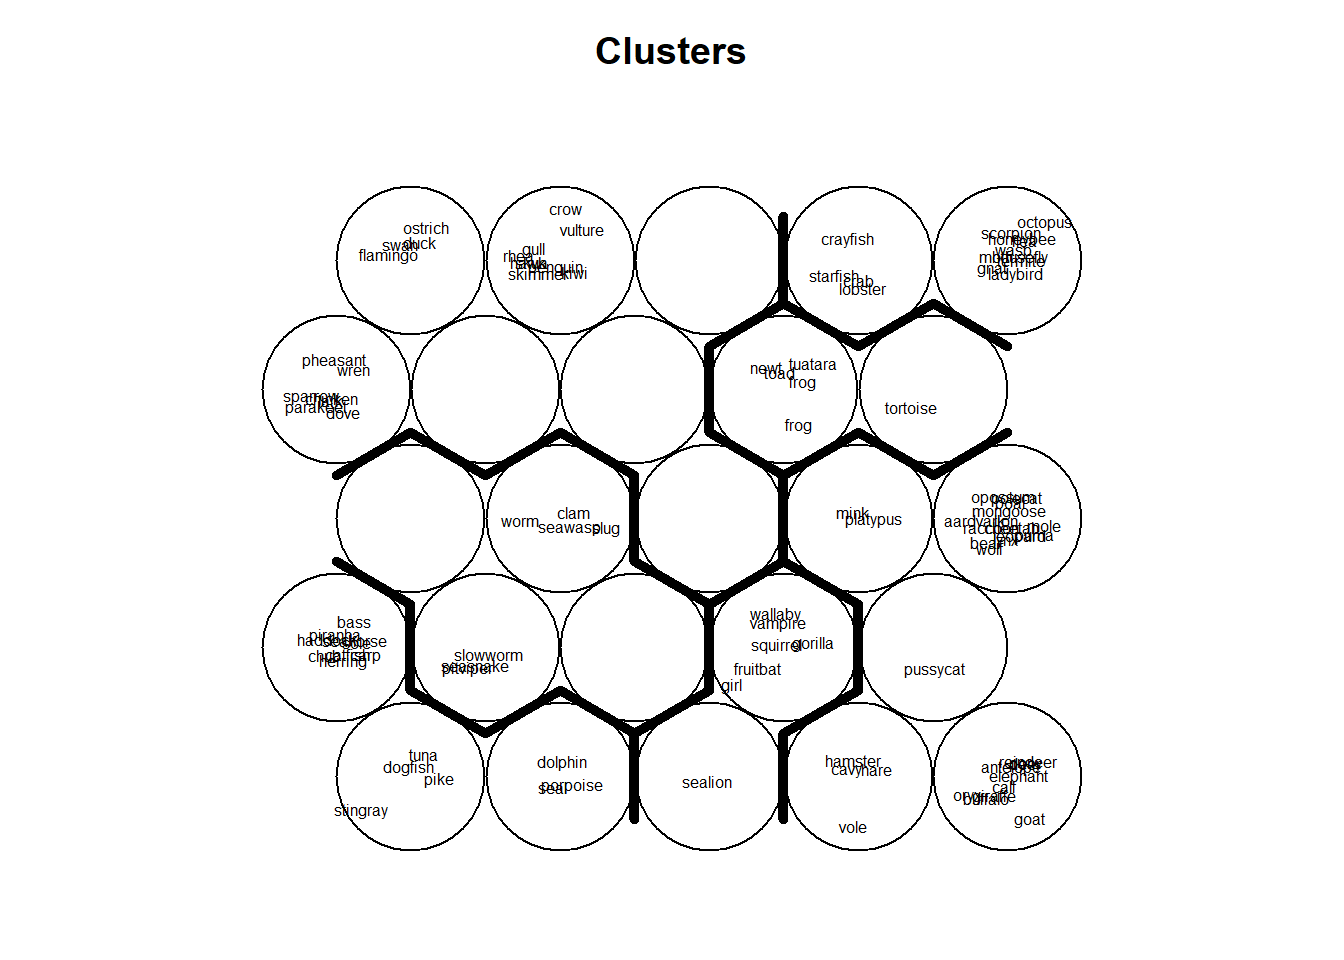
\includegraphics{Applied-Spatial-Data-Analysis_files/figure-latex/unnamed-chunk-53-1.pdf}

\hypertarget{simulated-regular-pattern-1}{%
\subsubsection{Simulated Regular Pattern}\label{simulated-regular-pattern-1}}

\begin{Shaded}
\begin{Highlighting}[]
\NormalTok{e2e\_regular }\OtherTok{=} \FunctionTok{nndist}\NormalTok{(pp\_regular)}
\NormalTok{e2e\_regular}
\end{Highlighting}
\end{Shaded}

\begin{verbatim}
##  [1] 0.1111111 0.1111111 0.1111111 0.1111111 0.1111111 0.1111111 0.1111111
##  [8] 0.1111111 0.1111111 0.1111111 0.1111111 0.1111111 0.1111111 0.1111111
## [15] 0.1111111 0.1111111 0.1111111 0.1111111 0.1111111 0.1111111 0.1111111
## [22] 0.1111111 0.1111111 0.1111111 0.1111111 0.1111111 0.1111111 0.1111111
## [29] 0.1111111 0.1111111 0.1111111 0.1111111 0.1111111 0.1111111 0.1111111
## [36] 0.1111111 0.1111111 0.1111111 0.1111111 0.1111111
\end{verbatim}

\begin{Shaded}
\begin{Highlighting}[]
\NormalTok{PD\_regular }\OtherTok{=} \FunctionTok{pairdist}\NormalTok{(pp\_regular)}
\FunctionTok{class}\NormalTok{(PD\_regular)}
\end{Highlighting}
\end{Shaded}

\begin{verbatim}
## [1] "matrix" "array"
\end{verbatim}

\begin{Shaded}
\begin{Highlighting}[]
\NormalTok{dm\_regular }\OtherTok{\textless{}{-}} \FunctionTok{as.matrix}\NormalTok{(PD\_regular)}
\NormalTok{dm\_regular[}\DecValTok{1}\SpecialCharTok{:}\DecValTok{5}\NormalTok{, }\DecValTok{1}\SpecialCharTok{:}\DecValTok{5}\NormalTok{]}
\end{Highlighting}
\end{Shaded}

\begin{verbatim}
##           [,1]      [,2]      [,3]      [,4]      [,5]
## [1,] 0.0000000 0.1666667 0.3333333 0.5000000 0.6666667
## [2,] 0.1666667 0.0000000 0.1666667 0.3333333 0.5000000
## [3,] 0.3333333 0.1666667 0.0000000 0.1666667 0.3333333
## [4,] 0.5000000 0.3333333 0.1666667 0.0000000 0.1666667
## [5,] 0.6666667 0.5000000 0.3333333 0.1666667 0.0000000
\end{verbatim}

\begin{Shaded}
\begin{Highlighting}[]
\FunctionTok{diag}\NormalTok{(dm\_regular) }\OtherTok{\textless{}{-}} \ConstantTok{NA}
\NormalTok{wdmin\_regular }\OtherTok{\textless{}{-}} \FunctionTok{apply}\NormalTok{(dm\_regular, }\DecValTok{1}\NormalTok{, which.min)}

\NormalTok{dmin\_regular }\OtherTok{\textless{}{-}} \FunctionTok{apply}\NormalTok{(dm\_regular, }\DecValTok{1}\NormalTok{, min, }\AttributeTok{na.rm=}\ConstantTok{TRUE}\NormalTok{)}
\FunctionTok{head}\NormalTok{(dmin}\SpecialCharTok{{-}}\NormalTok{regular)}
\end{Highlighting}
\end{Shaded}

\begin{verbatim}
##             X             Y
## 1 -0.05610447 -0.0005489143
## 2 -0.27914228 -0.0569200607
## 3 -0.41836751 -0.0294786165
## 4 -0.61092147 -0.0553659112
## 5 -0.63425768  0.0879645408
## 6 -0.13475501 -0.1903105666
\end{verbatim}

\begin{Shaded}
\begin{Highlighting}[]
\CommentTok{\# which is the same as nndist e2e=nndist(swp)}

\NormalTok{dmin\_regular }\OtherTok{=} \FunctionTok{nndist}\NormalTok{(pp\_regular)}

\FunctionTok{plot}\NormalTok{(pp\_regular)}
\NormalTok{xy\_regular }\OtherTok{=} \FunctionTok{cbind}\NormalTok{(pp\_regular}\SpecialCharTok{$}\NormalTok{x, pp\_regular}\SpecialCharTok{$}\NormalTok{y)}

\NormalTok{ord }\OtherTok{\textless{}{-}} \FunctionTok{rev}\NormalTok{(}\FunctionTok{order}\NormalTok{(dmin\_regular))}
\NormalTok{far25 }\OtherTok{\textless{}{-}}\NormalTok{ ord[}\DecValTok{1}\SpecialCharTok{:}\DecValTok{40}\NormalTok{]}
\NormalTok{neighbors }\OtherTok{\textless{}{-}}\NormalTok{ wdmin\_regular[far25]}
\FunctionTok{points}\NormalTok{(xy\_regular[far25, ], }\AttributeTok{col=}\StringTok{\textquotesingle{}blue\textquotesingle{}}\NormalTok{, }\AttributeTok{pch=}\DecValTok{20}\NormalTok{)}
\FunctionTok{points}\NormalTok{(xy\_regular[neighbors, ], }\AttributeTok{col=}\StringTok{\textquotesingle{}red\textquotesingle{}}\NormalTok{)}
\CommentTok{\# drawing the lines, easiest via a loop}
\ControlFlowTok{for}\NormalTok{ (i }\ControlFlowTok{in}\NormalTok{ far25) \{}
    \FunctionTok{lines}\NormalTok{(}\FunctionTok{rbind}\NormalTok{(xy\_regular[i, ], xy\_regular[wdmin\_regular[i], ]), }\AttributeTok{col=}\StringTok{\textquotesingle{}red\textquotesingle{}}\NormalTok{)}
\NormalTok{\}}
\end{Highlighting}
\end{Shaded}

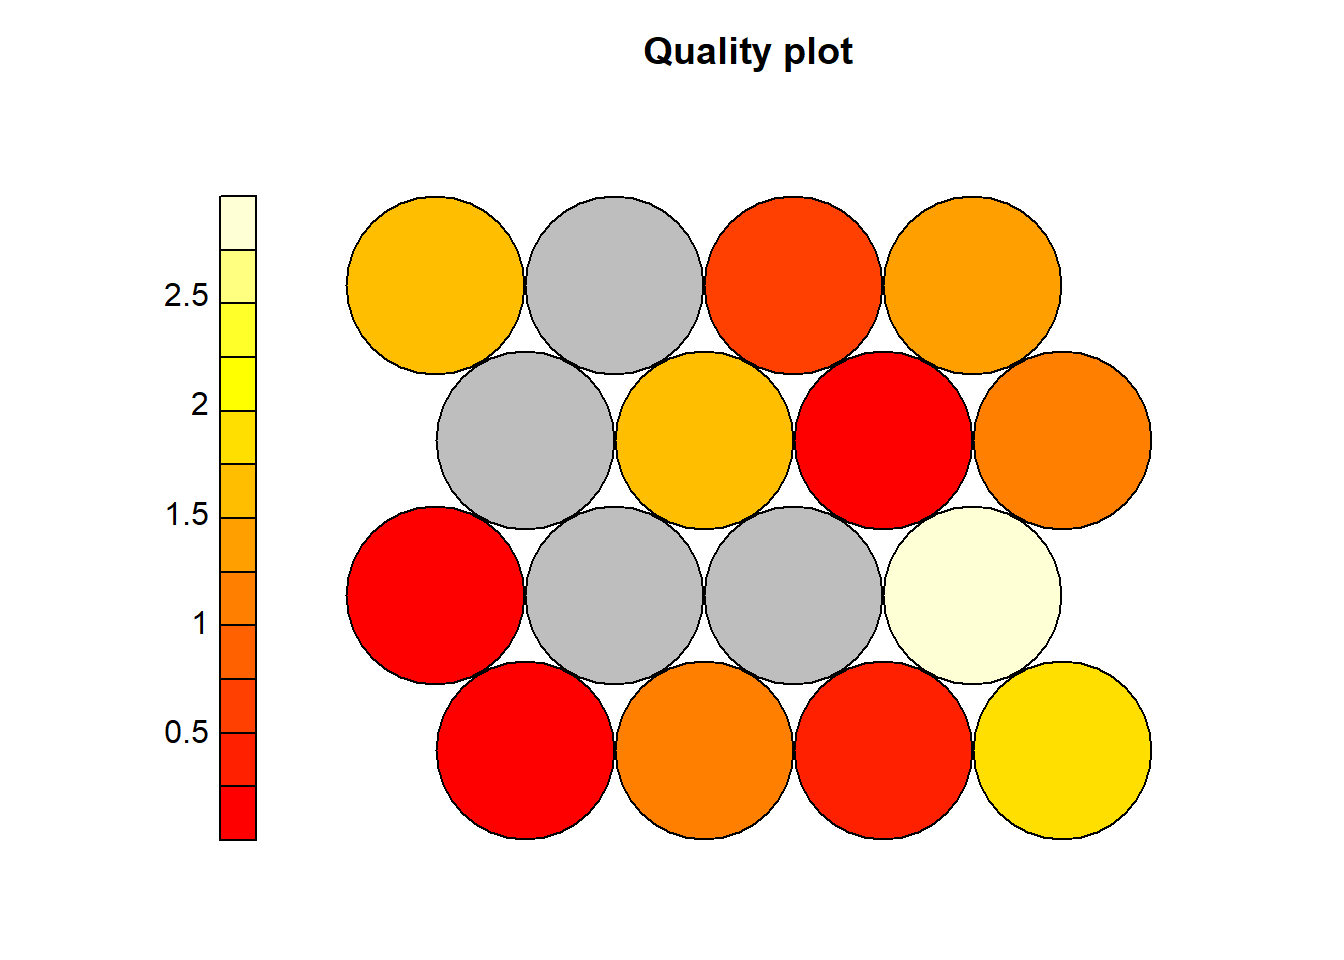
\includegraphics{Applied-Spatial-Data-Analysis_files/figure-latex/unnamed-chunk-55-1.pdf}

\hypertarget{p2e-distances}{%
\subsection{p2e Distances}\label{p2e-distances}}

Generate Random points

\begin{Shaded}
\begin{Highlighting}[]
\FunctionTok{set.seed}\NormalTok{(}\DecValTok{23}\NormalTok{)}
\NormalTok{randompoints }\OtherTok{=} \FunctionTok{matrix}\NormalTok{(}\FunctionTok{runif}\NormalTok{(}\DecValTok{60}\NormalTok{),}\AttributeTok{ncol=}\DecValTok{2}\NormalTok{)}
\CommentTok{\#randompoints = matrix(runif(250),ncol=2)}
\end{Highlighting}
\end{Shaded}

\hypertarget{csr-pattern-1}{%
\subsubsection{CSR Pattern}\label{csr-pattern-1}}

\begin{Shaded}
\begin{Highlighting}[]
\FunctionTok{plot}\NormalTok{(pp\_csr)}
\FunctionTok{points}\NormalTok{(randompoints, }\AttributeTok{col =} \StringTok{"blue"}\NormalTok{, }\AttributeTok{pch=}\DecValTok{3}\NormalTok{)}
\end{Highlighting}
\end{Shaded}

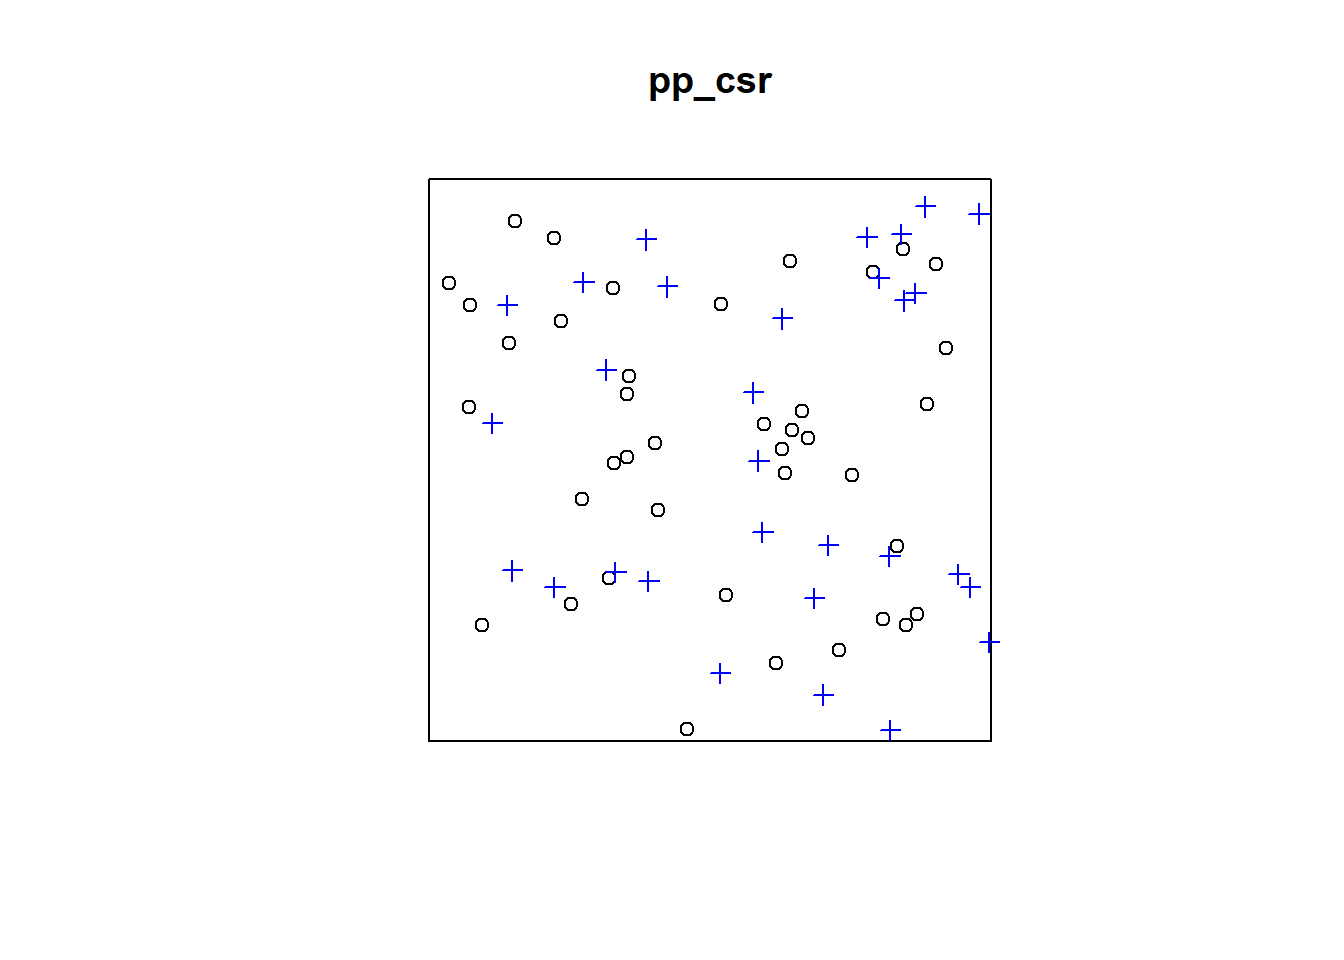
\includegraphics{Applied-Spatial-Data-Analysis_files/figure-latex/unnamed-chunk-57-1.pdf}

\begin{Shaded}
\begin{Highlighting}[]
\NormalTok{p2e\_distances\_csr }\OtherTok{=} \ConstantTok{NULL}
\NormalTok{mins\_csr }\OtherTok{=} \ConstantTok{NULL}
\NormalTok{xy }\OtherTok{=} \FunctionTok{cbind}\NormalTok{(pp\_csr}\SpecialCharTok{$}\NormalTok{x, pp\_csr}\SpecialCharTok{$}\NormalTok{y)}


\CommentTok{\# sqrt((xy[2,1]{-}randompoints[1,1])\^{}2+(xy[2,2]{-}randompoints[1,2])\^{}2)}
\CommentTok{\# sqrt((xy[1,1]{-}randompoints[2,1])\^{}2+(xy[1,2]{-}randompoints[2,2])\^{}2)}


\ControlFlowTok{for}\NormalTok{(i }\ControlFlowTok{in} \DecValTok{1}\SpecialCharTok{:}\FunctionTok{dim}\NormalTok{(randompoints)[}\DecValTok{1}\NormalTok{])\{}
\NormalTok{dist1 }\OtherTok{=} \FunctionTok{matrix}\NormalTok{(}\FunctionTok{pairdist}\NormalTok{(}\FunctionTok{rbind}\NormalTok{(randompoints[i,],xy)),}\DecValTok{41}\NormalTok{)}

\NormalTok{p2e\_distances\_csr }\OtherTok{=} \FunctionTok{c}\NormalTok{(p2e\_distances\_csr,}\FunctionTok{min}\NormalTok{(dist1[}\DecValTok{2}\SpecialCharTok{:}\DecValTok{41}\NormalTok{,}\DecValTok{1}\NormalTok{]))}
\NormalTok{mins\_csr }\OtherTok{=} \FunctionTok{c}\NormalTok{(mins\_csr,}\FunctionTok{which.min}\NormalTok{(dist1[}\DecValTok{2}\SpecialCharTok{:}\DecValTok{41}\NormalTok{,}\DecValTok{1}\NormalTok{]))}
\NormalTok{\}}


\FunctionTok{plot}\NormalTok{(pp\_csr)}
\NormalTok{ord }\OtherTok{\textless{}{-}} \FunctionTok{rev}\NormalTok{(}\FunctionTok{order}\NormalTok{(p2e\_distances\_csr))}
\NormalTok{far25 }\OtherTok{\textless{}{-}} \DecValTok{1}\SpecialCharTok{:}\FunctionTok{dim}\NormalTok{(randompoints)[}\DecValTok{1}\NormalTok{]}
\NormalTok{neighbors }\OtherTok{\textless{}{-}}\NormalTok{ mins\_csr}
\FunctionTok{points}\NormalTok{(randompoints, }\AttributeTok{col=}\StringTok{\textquotesingle{}red\textquotesingle{}}\NormalTok{, }\AttributeTok{pch=}\DecValTok{4}\NormalTok{)}
\FunctionTok{points}\NormalTok{(xy[mins\_csr, ], }\AttributeTok{col=}\StringTok{\textquotesingle{}blue\textquotesingle{}}\NormalTok{, }\AttributeTok{pch=}\DecValTok{20}\NormalTok{)}
\CommentTok{\# drawing the lines, easiest via a loop}
\ControlFlowTok{for}\NormalTok{ (i }\ControlFlowTok{in}\NormalTok{ far25) \{}
  \FunctionTok{lines}\NormalTok{(}\FunctionTok{rbind}\NormalTok{(xy[mins\_csr[i], ], randompoints[i, ]), }\AttributeTok{col=}\StringTok{\textquotesingle{}red\textquotesingle{}}\NormalTok{)}
\NormalTok{\}}
\end{Highlighting}
\end{Shaded}

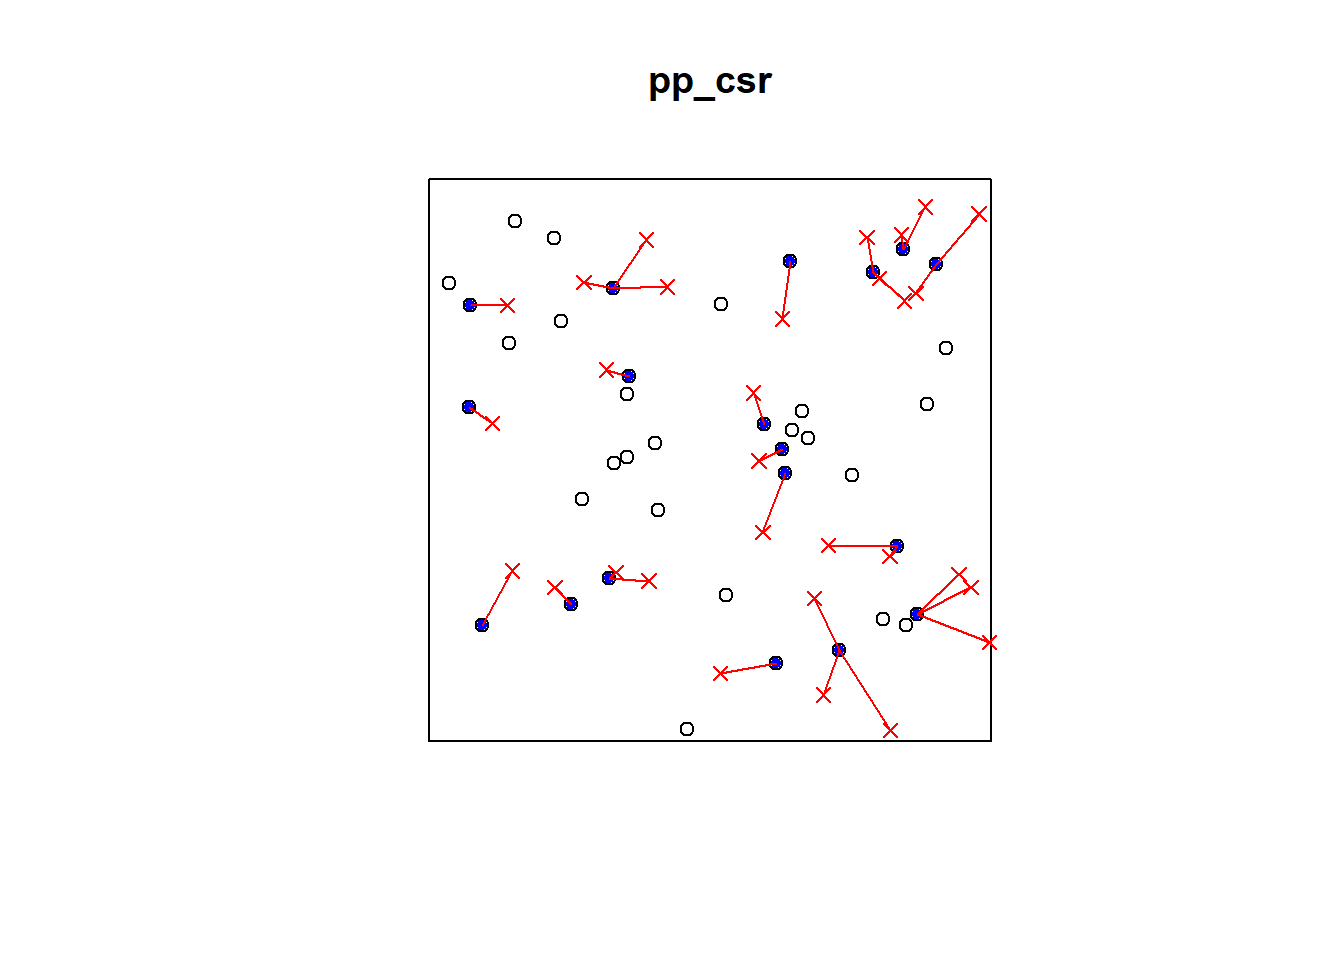
\includegraphics{Applied-Spatial-Data-Analysis_files/figure-latex/unnamed-chunk-58-1.pdf}

\hypertarget{cluster-pattern-1}{%
\subsubsection{Cluster Pattern}\label{cluster-pattern-1}}

\begin{Shaded}
\begin{Highlighting}[]
\FunctionTok{plot}\NormalTok{(pp\_cluster)}
\FunctionTok{points}\NormalTok{(randompoints, }\AttributeTok{col =} \StringTok{"blue"}\NormalTok{, }\AttributeTok{pch=}\DecValTok{3}\NormalTok{)}
\end{Highlighting}
\end{Shaded}

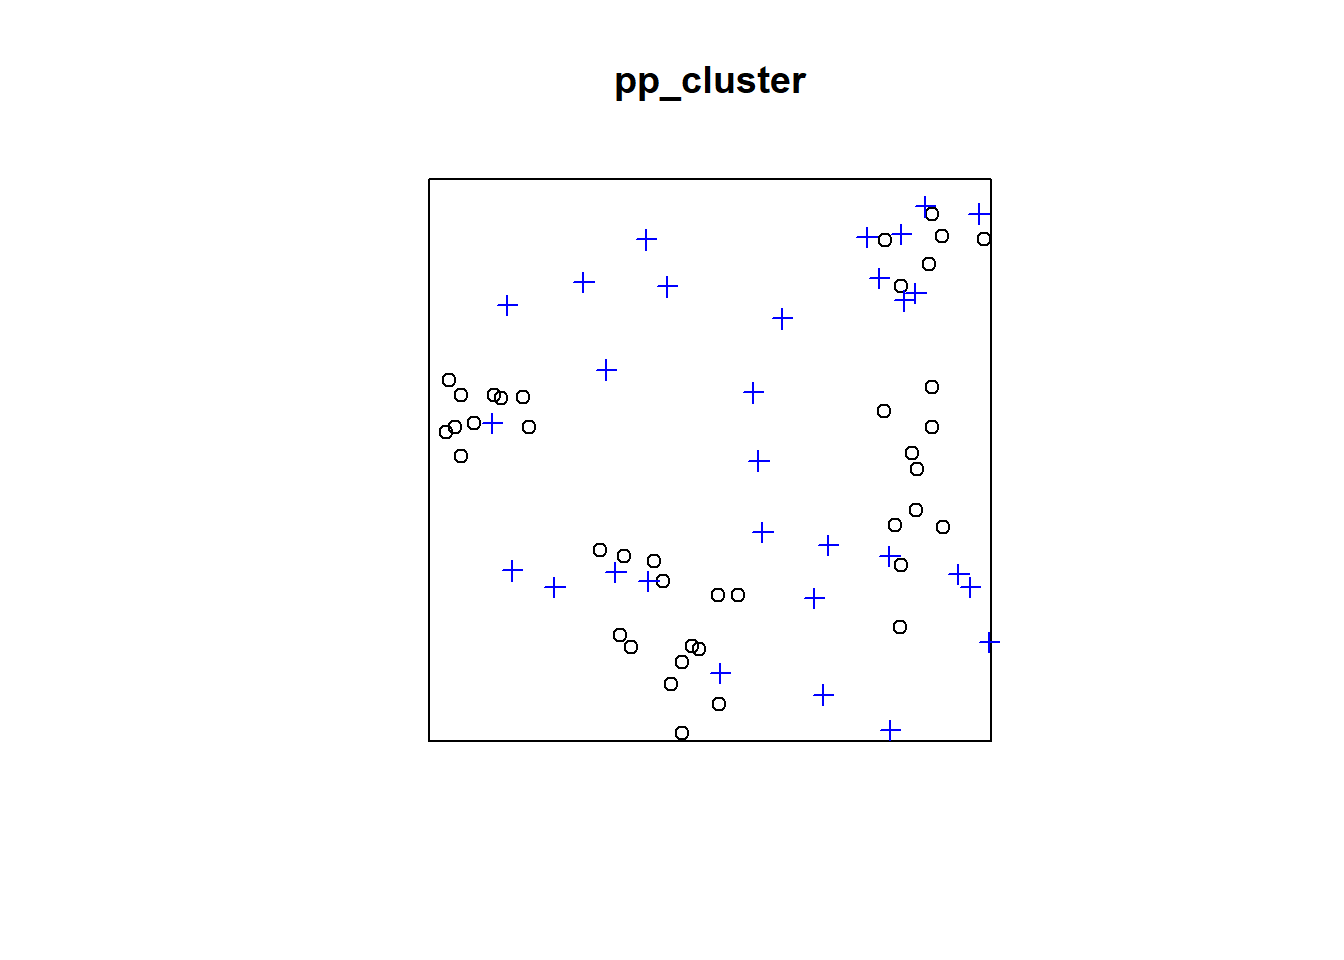
\includegraphics{Applied-Spatial-Data-Analysis_files/figure-latex/unnamed-chunk-59-1.pdf}

\begin{Shaded}
\begin{Highlighting}[]
\NormalTok{p2e\_distances\_cluster }\OtherTok{=} \ConstantTok{NULL}
\NormalTok{mins\_cluster }\OtherTok{=} \ConstantTok{NULL}
\NormalTok{xy\_cluster }\OtherTok{=} \FunctionTok{cbind}\NormalTok{(pp\_cluster}\SpecialCharTok{$}\NormalTok{x, pp\_cluster}\SpecialCharTok{$}\NormalTok{y)}

\ControlFlowTok{for}\NormalTok{(i }\ControlFlowTok{in} \DecValTok{1}\SpecialCharTok{:}\FunctionTok{dim}\NormalTok{(randompoints)[}\DecValTok{1}\NormalTok{])\{}
\NormalTok{dist1 }\OtherTok{=} \FunctionTok{matrix}\NormalTok{(}\FunctionTok{pairdist}\NormalTok{(}\FunctionTok{rbind}\NormalTok{(randompoints[i,],xy\_cluster)),}\DecValTok{41}\NormalTok{)}

\NormalTok{p2e\_distances\_cluster }\OtherTok{=} \FunctionTok{c}\NormalTok{(p2e\_distances\_cluster,}\FunctionTok{min}\NormalTok{(dist1[}\DecValTok{2}\SpecialCharTok{:}\DecValTok{41}\NormalTok{,}\DecValTok{1}\NormalTok{]))}
\NormalTok{mins\_cluster }\OtherTok{=} \FunctionTok{c}\NormalTok{(mins\_cluster,}\FunctionTok{which.min}\NormalTok{(dist1[}\DecValTok{2}\SpecialCharTok{:}\DecValTok{41}\NormalTok{,}\DecValTok{1}\NormalTok{]))}
\NormalTok{\}}


\FunctionTok{plot}\NormalTok{(pp\_cluster)}
\NormalTok{ord }\OtherTok{\textless{}{-}} \FunctionTok{rev}\NormalTok{(}\FunctionTok{order}\NormalTok{(p2e\_distances\_cluster))}
\NormalTok{far25 }\OtherTok{\textless{}{-}} \DecValTok{1}\SpecialCharTok{:}\FunctionTok{dim}\NormalTok{(randompoints)[}\DecValTok{1}\NormalTok{]}
\NormalTok{neighbors }\OtherTok{\textless{}{-}}\NormalTok{ mins\_cluster}
\FunctionTok{points}\NormalTok{(randompoints, }\AttributeTok{col=}\StringTok{\textquotesingle{}red\textquotesingle{}}\NormalTok{, }\AttributeTok{pch=}\DecValTok{4}\NormalTok{)}
\FunctionTok{points}\NormalTok{(xy\_cluster[mins\_cluster, ], }\AttributeTok{col=}\StringTok{\textquotesingle{}blue\textquotesingle{}}\NormalTok{, }\AttributeTok{pch=}\DecValTok{20}\NormalTok{)}
\CommentTok{\# drawing the lines, easiest via a loop}
\ControlFlowTok{for}\NormalTok{ (i }\ControlFlowTok{in}\NormalTok{ far25) \{}
  \FunctionTok{lines}\NormalTok{(}\FunctionTok{rbind}\NormalTok{(xy\_cluster[mins\_cluster[i], ], randompoints[i, ]), }\AttributeTok{col=}\StringTok{\textquotesingle{}red\textquotesingle{}}\NormalTok{)}
\NormalTok{\}}
\end{Highlighting}
\end{Shaded}

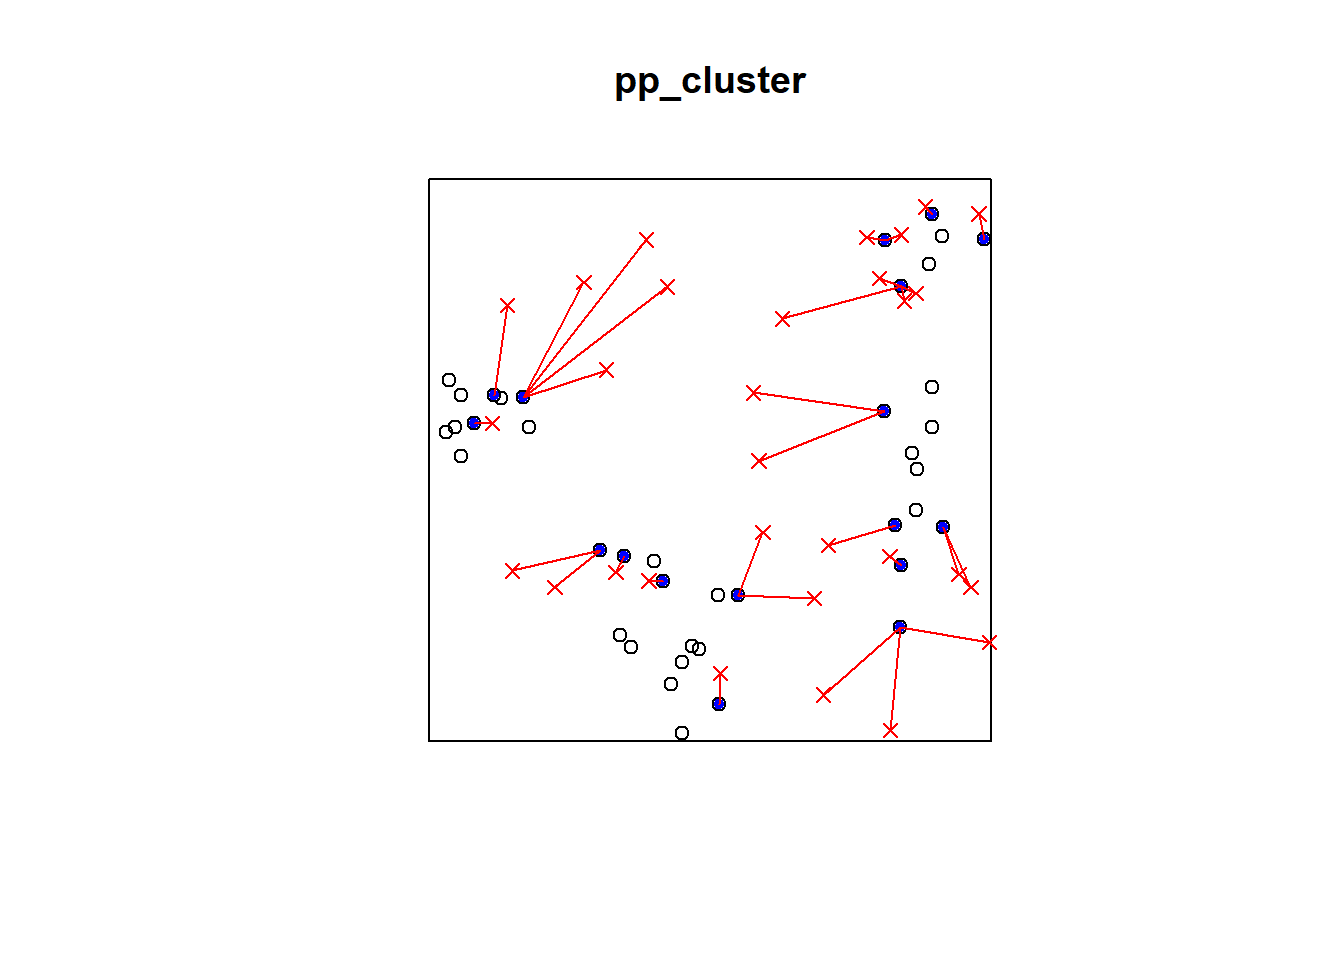
\includegraphics{Applied-Spatial-Data-Analysis_files/figure-latex/unnamed-chunk-60-1.pdf}

\hypertarget{regular-pattern-1}{%
\subsubsection{Regular Pattern}\label{regular-pattern-1}}

\begin{Shaded}
\begin{Highlighting}[]
\NormalTok{p2e\_distances\_regular }\OtherTok{=} \ConstantTok{NULL}
\NormalTok{p2e\_mins\_regular }\OtherTok{=} \ConstantTok{NULL}
\NormalTok{xy\_regular }\OtherTok{=} \FunctionTok{cbind}\NormalTok{(pp\_regular}\SpecialCharTok{$}\NormalTok{x, pp\_regular}\SpecialCharTok{$}\NormalTok{y)}


\ControlFlowTok{for}\NormalTok{(i }\ControlFlowTok{in} \DecValTok{1}\SpecialCharTok{:}\FunctionTok{dim}\NormalTok{(randompoints)[}\DecValTok{1}\NormalTok{])\{}
\NormalTok{dist1 }\OtherTok{=} \FunctionTok{matrix}\NormalTok{(}\FunctionTok{pairdist}\NormalTok{(}\FunctionTok{rbind}\NormalTok{(randompoints[i,],xy\_regular)),}\DecValTok{41}\NormalTok{)}

\NormalTok{p2e\_distances\_regular }\OtherTok{=} \FunctionTok{c}\NormalTok{(p2e\_distances\_regular,}\FunctionTok{min}\NormalTok{(dist1[}\DecValTok{2}\SpecialCharTok{:}\DecValTok{41}\NormalTok{,}\DecValTok{1}\NormalTok{]))}
\NormalTok{p2e\_mins\_regular }\OtherTok{=} \FunctionTok{c}\NormalTok{(p2e\_mins\_regular,}\FunctionTok{which.min}\NormalTok{(dist1[}\DecValTok{2}\SpecialCharTok{:}\DecValTok{41}\NormalTok{,}\DecValTok{1}\NormalTok{]))}
\NormalTok{\}}


\FunctionTok{plot}\NormalTok{(pp\_regular)}
\NormalTok{ord }\OtherTok{\textless{}{-}} \FunctionTok{rev}\NormalTok{(}\FunctionTok{order}\NormalTok{(p2e\_distances\_regular))}
\NormalTok{far25 }\OtherTok{\textless{}{-}} \DecValTok{1}\SpecialCharTok{:}\FunctionTok{dim}\NormalTok{(randompoints)[}\DecValTok{1}\NormalTok{]}
\NormalTok{neighbors }\OtherTok{\textless{}{-}}\NormalTok{ p2e\_mins\_regular}
\FunctionTok{points}\NormalTok{(randompoints, }\AttributeTok{col=}\StringTok{\textquotesingle{}red\textquotesingle{}}\NormalTok{, }\AttributeTok{pch=}\DecValTok{4}\NormalTok{)}
\FunctionTok{points}\NormalTok{(xy\_regular[p2e\_mins\_regular, ], }\AttributeTok{col=}\StringTok{\textquotesingle{}blue\textquotesingle{}}\NormalTok{, }\AttributeTok{pch=}\DecValTok{20}\NormalTok{)}
\CommentTok{\# drawing the lines, easiest via a loop}
\ControlFlowTok{for}\NormalTok{ (i }\ControlFlowTok{in}\NormalTok{ far25) \{}
  \FunctionTok{lines}\NormalTok{(}\FunctionTok{rbind}\NormalTok{(xy\_regular[p2e\_mins\_regular[i], ], randompoints[i, ]), }\AttributeTok{col=}\StringTok{\textquotesingle{}red\textquotesingle{}}\NormalTok{)}
\NormalTok{\}}
\end{Highlighting}
\end{Shaded}

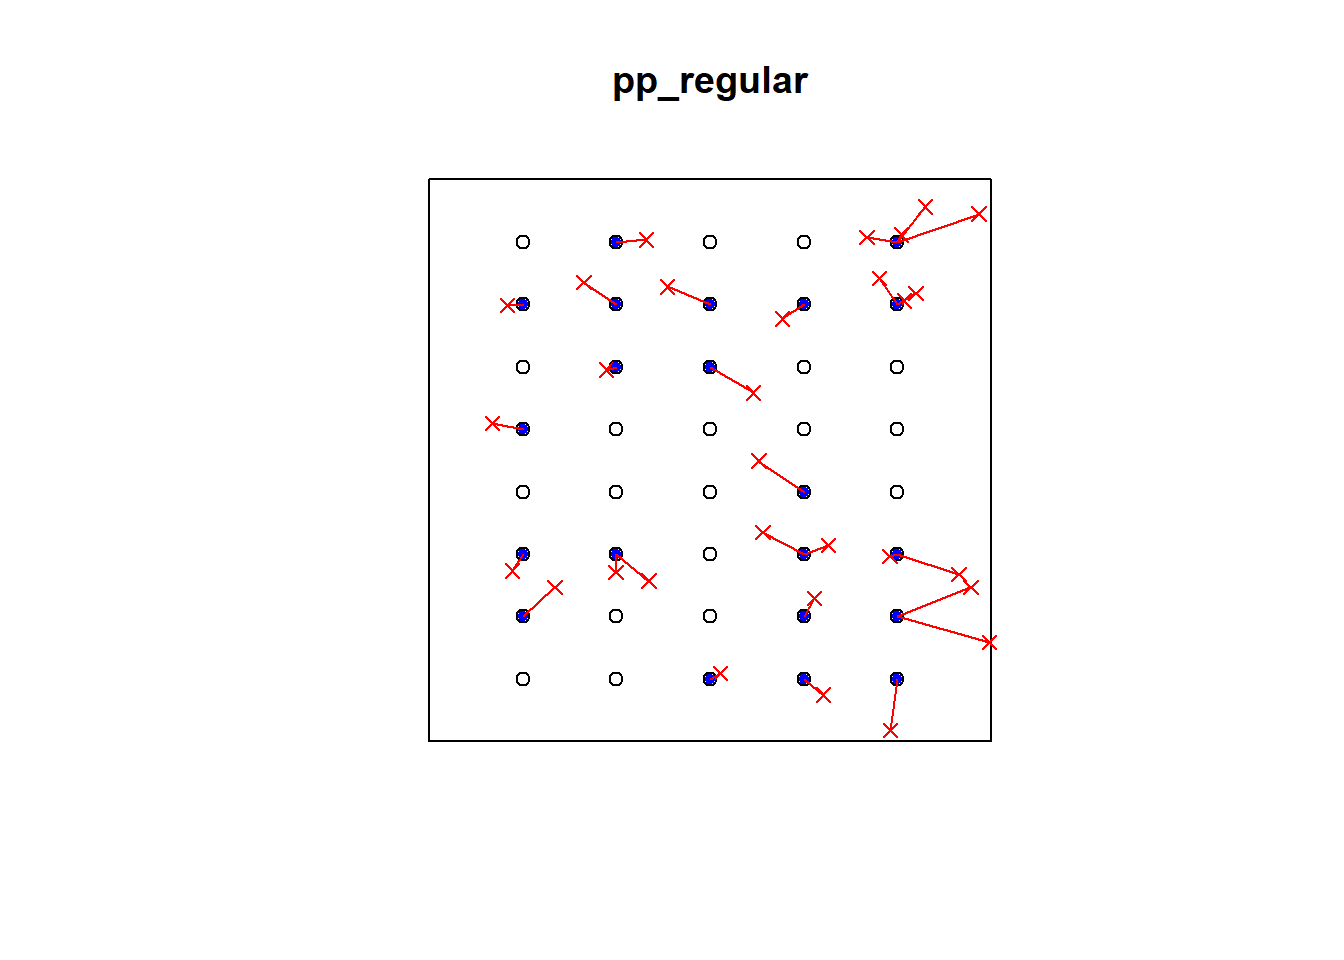
\includegraphics{Applied-Spatial-Data-Analysis_files/figure-latex/unnamed-chunk-61-1.pdf}

\hypertarget{clark-and-evans-index-and-test}{%
\subsection{Clark and Evans Index and Test}\label{clark-and-evans-index-and-test}}

\hypertarget{csr-pattern-2}{%
\subsubsection{CSR Pattern}\label{csr-pattern-2}}

\begin{Shaded}
\begin{Highlighting}[]
\FunctionTok{clarkevans}\NormalTok{(pp\_csr)}
\end{Highlighting}
\end{Shaded}

\begin{verbatim}
##     naive  Donnelly       cdf 
## 1.0135515 0.9443703 0.9719128
\end{verbatim}

\begin{Shaded}
\begin{Highlighting}[]
\FunctionTok{clarkevans.test}\NormalTok{(pp\_csr)}
\end{Highlighting}
\end{Shaded}

\begin{verbatim}
## 
##  Clark-Evans test
##  No edge correction
##  Z-test
## 
## data:  pp_csr
## R = 1.0136, p-value = 0.8698
## alternative hypothesis: two-sided
\end{verbatim}

\hypertarget{cluster-pattern-2}{%
\subsubsection{Cluster Pattern}\label{cluster-pattern-2}}

\begin{Shaded}
\begin{Highlighting}[]
\FunctionTok{clarkevans}\NormalTok{(pp\_cluster)}
\end{Highlighting}
\end{Shaded}

\begin{verbatim}
##     naive  Donnelly       cdf 
## 0.5852722 0.5453237 0.5621148
\end{verbatim}

\begin{Shaded}
\begin{Highlighting}[]
\FunctionTok{clarkevans.test}\NormalTok{(pp\_cluster)}
\end{Highlighting}
\end{Shaded}

\begin{verbatim}
## 
##  Clark-Evans test
##  No edge correction
##  Z-test
## 
## data:  pp_cluster
## R = 0.58527, p-value = 5.224e-07
## alternative hypothesis: two-sided
\end{verbatim}

\hypertarget{regular-pattern-2}{%
\subsubsection{Regular Pattern}\label{regular-pattern-2}}

\begin{Shaded}
\begin{Highlighting}[]
\FunctionTok{clarkevans}\NormalTok{(pp\_regular)}
\end{Highlighting}
\end{Shaded}

\begin{verbatim}
##    naive Donnelly      cdf 
## 1.405457 1.309526 1.398362
\end{verbatim}

\begin{Shaded}
\begin{Highlighting}[]
\FunctionTok{clarkevans.test}\NormalTok{(pp\_regular)}
\end{Highlighting}
\end{Shaded}

\begin{verbatim}
## 
##  Clark-Evans test
##  No edge correction
##  Z-test
## 
## data:  pp_regular
## R = 1.4055, p-value = 9.309e-07
## alternative hypothesis: two-sided
\end{verbatim}

\hypertarget{g-function}{%
\section{G Function}\label{g-function}}

\hypertarget{simulated-csr-pattern-2}{%
\subsection{Simulated CSR Pattern}\label{simulated-csr-pattern-2}}

\begin{Shaded}
\begin{Highlighting}[]
\FunctionTok{plot}\NormalTok{(}\FunctionTok{Gest}\NormalTok{(pp\_csr))}
\end{Highlighting}
\end{Shaded}

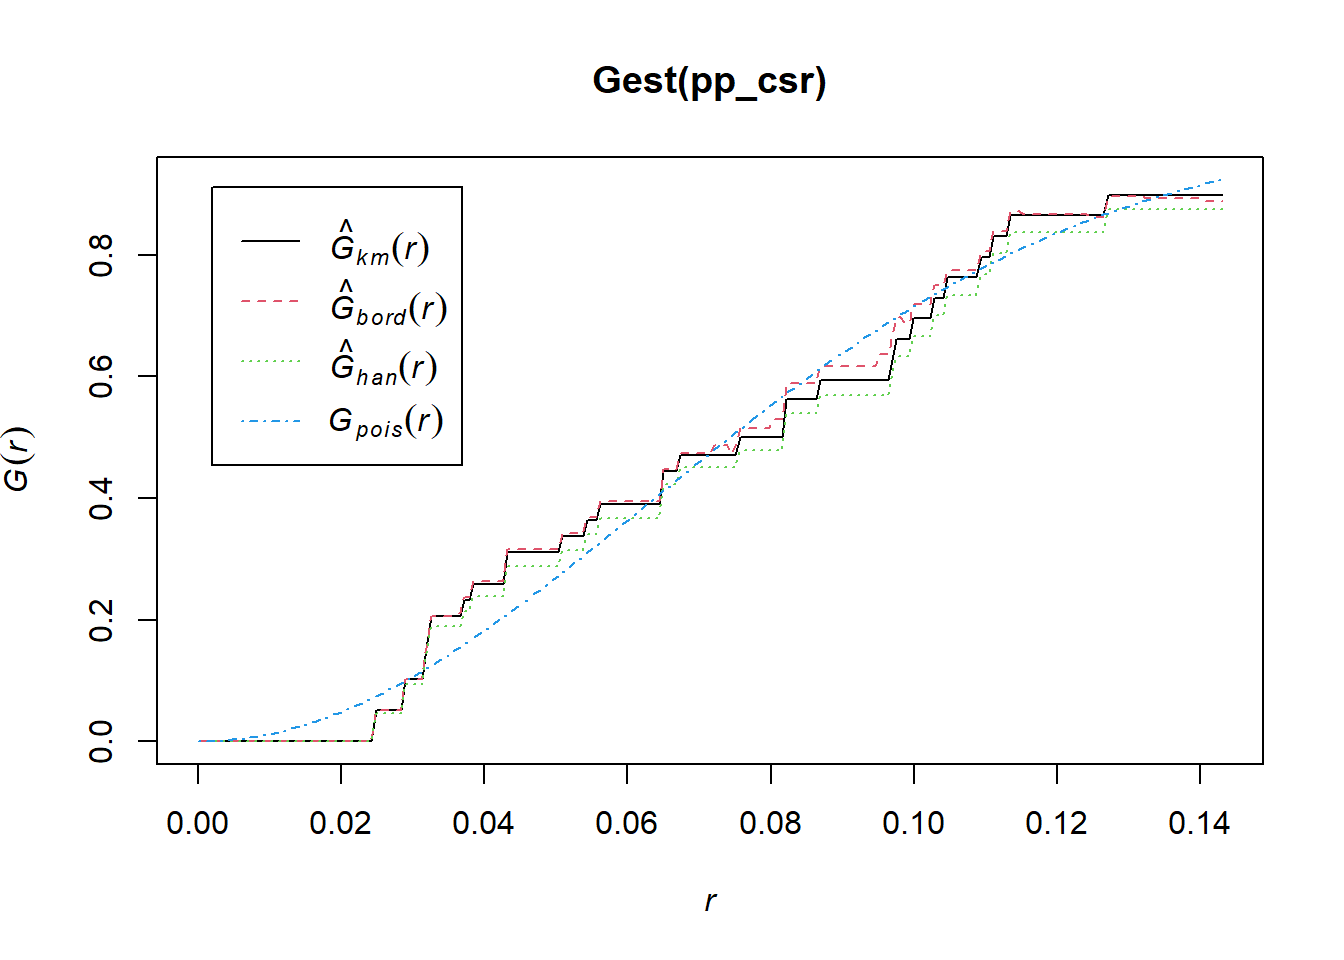
\includegraphics{Applied-Spatial-Data-Analysis_files/figure-latex/unnamed-chunk-65-1.pdf}

\hypertarget{simulated-regular-pattern-2}{%
\subsection{Simulated Regular Pattern}\label{simulated-regular-pattern-2}}

\begin{Shaded}
\begin{Highlighting}[]
\FunctionTok{plot}\NormalTok{(}\FunctionTok{Gest}\NormalTok{(pp\_regular))}
\end{Highlighting}
\end{Shaded}

\includegraphics{Applied-Spatial-Data-Analysis_files/figure-latex/unnamed-chunk-66-1.pdf}

\hypertarget{simulated-cluster-pattern-2}{%
\subsection{Simulated Cluster Pattern}\label{simulated-cluster-pattern-2}}

\begin{Shaded}
\begin{Highlighting}[]
\FunctionTok{plot}\NormalTok{(}\FunctionTok{Gest}\NormalTok{(pp\_cluster))}
\end{Highlighting}
\end{Shaded}

\includegraphics{Applied-Spatial-Data-Analysis_files/figure-latex/unnamed-chunk-67-1.pdf}

\hypertarget{f-function}{%
\section{F Function}\label{f-function}}

\hypertarget{simulated-csr-pattern-3}{%
\subsection{Simulated CSR Pattern}\label{simulated-csr-pattern-3}}

\begin{Shaded}
\begin{Highlighting}[]
\FunctionTok{plot}\NormalTok{(}\FunctionTok{Fest}\NormalTok{(pp\_csr))}
\end{Highlighting}
\end{Shaded}

\includegraphics{Applied-Spatial-Data-Analysis_files/figure-latex/unnamed-chunk-68-1.pdf}

\hypertarget{simulated-regular-pattern-3}{%
\subsection{Simulated Regular Pattern}\label{simulated-regular-pattern-3}}

\begin{Shaded}
\begin{Highlighting}[]
\FunctionTok{plot}\NormalTok{(}\FunctionTok{Fest}\NormalTok{(pp\_regular))}
\end{Highlighting}
\end{Shaded}

\includegraphics{Applied-Spatial-Data-Analysis_files/figure-latex/unnamed-chunk-69-1.pdf}

\hypertarget{simulated-cluster-pattern-3}{%
\subsection{Simulated Cluster Pattern}\label{simulated-cluster-pattern-3}}

\begin{Shaded}
\begin{Highlighting}[]
\FunctionTok{plot}\NormalTok{(}\FunctionTok{Fest}\NormalTok{(pp\_cluster))}
\end{Highlighting}
\end{Shaded}

\includegraphics{Applied-Spatial-Data-Analysis_files/figure-latex/unnamed-chunk-70-1.pdf}

\hypertarget{ripleys-k-function}{%
\section{Ripley's K Function}\label{ripleys-k-function}}

\hypertarget{simulated-csr-pattern-4}{%
\subsection{Simulated CSR Pattern}\label{simulated-csr-pattern-4}}

\begin{Shaded}
\begin{Highlighting}[]
\NormalTok{K }\OtherTok{\textless{}{-}} \FunctionTok{Kest}\NormalTok{(pp\_csr)}
\FunctionTok{plot}\NormalTok{(K, }\AttributeTok{main=}\ConstantTok{NULL}\NormalTok{, }\AttributeTok{las=}\DecValTok{1}\NormalTok{, }\AttributeTok{legendargs=}\FunctionTok{list}\NormalTok{(}\AttributeTok{cex=}\FloatTok{0.8}\NormalTok{, }\AttributeTok{xpd=}\ConstantTok{TRUE}\NormalTok{, }\AttributeTok{inset=}\FunctionTok{c}\NormalTok{(}\FloatTok{1.01}\NormalTok{, }\DecValTok{0}\NormalTok{) ))}
\end{Highlighting}
\end{Shaded}

\begin{verbatim}
## Warning in min(D[scaledlegbox]): no non-missing arguments to min; returning Inf
\end{verbatim}

\includegraphics{Applied-Spatial-Data-Analysis_files/figure-latex/unnamed-chunk-71-1.pdf}

\hypertarget{simulated-regular-pattern-4}{%
\subsection{Simulated Regular Pattern}\label{simulated-regular-pattern-4}}

\begin{Shaded}
\begin{Highlighting}[]
\NormalTok{K }\OtherTok{\textless{}{-}} \FunctionTok{Kest}\NormalTok{(pp\_regular)}
\FunctionTok{plot}\NormalTok{(K, }\AttributeTok{main=}\ConstantTok{NULL}\NormalTok{, }\AttributeTok{las=}\DecValTok{1}\NormalTok{, }\AttributeTok{legendargs=}\FunctionTok{list}\NormalTok{(}\AttributeTok{cex=}\FloatTok{0.8}\NormalTok{, }\AttributeTok{xpd=}\ConstantTok{TRUE}\NormalTok{, }\AttributeTok{inset=}\FunctionTok{c}\NormalTok{(}\FloatTok{1.01}\NormalTok{, }\DecValTok{0}\NormalTok{) ))}
\end{Highlighting}
\end{Shaded}

\begin{verbatim}
## Warning in min(D[scaledlegbox]): no non-missing arguments to min; returning Inf
\end{verbatim}

\includegraphics{Applied-Spatial-Data-Analysis_files/figure-latex/unnamed-chunk-72-1.pdf}

\hypertarget{simulated-cluster-pattern-4}{%
\subsection{Simulated Cluster Pattern}\label{simulated-cluster-pattern-4}}

\begin{Shaded}
\begin{Highlighting}[]
\NormalTok{K }\OtherTok{\textless{}{-}} \FunctionTok{Kest}\NormalTok{(pp\_cluster)}
\FunctionTok{plot}\NormalTok{(K, }\AttributeTok{main=}\ConstantTok{NULL}\NormalTok{, }\AttributeTok{las=}\DecValTok{1}\NormalTok{, }\AttributeTok{legendargs=}\FunctionTok{list}\NormalTok{(}\AttributeTok{cex=}\FloatTok{0.8}\NormalTok{, }\AttributeTok{xpd=}\ConstantTok{TRUE}\NormalTok{, }\AttributeTok{inset=}\FunctionTok{c}\NormalTok{(}\FloatTok{1.01}\NormalTok{, }\DecValTok{0}\NormalTok{) ))}
\end{Highlighting}
\end{Shaded}

\begin{verbatim}
## Warning in min(D[scaledlegbox]): no non-missing arguments to min; returning Inf
\end{verbatim}

\includegraphics{Applied-Spatial-Data-Analysis_files/figure-latex/unnamed-chunk-73-1.pdf}

\hypertarget{references}{%
\section{References:}\label{references}}

\begin{itemize}
\item
  \href{https://rpubs.com/spring19cp6521/Week11_Wednesday1}{Point Pattern Analysis by Yongsung Lee}
\item
  \href{https://bookdown.org/lexcomber/brunsdoncomber2e/Ch6.html}{An Introduction to Spatial Analysis and Mapping in R 2nd edition by Chris Brunsdon and Lex Comber}
\item
  \href{https://mgimond.github.io/Spatial/point-pattern-analysis-in-r.html}{SPP in R by Manuel Gimond}
\item
  \href{https://yihui.org/animation/example/animation-package/}{Animation}
\item
  \href{https://skirmer.github.io/animation_prez.html\#1}{Animation}
\item
  \href{https://research.csiro.au/software/wp-content/uploads/sites/6/2015/02/Rspatialcourse_CMIS_PDF-Standard.pdf}{Baddeley}
\item
  \href{http://book.spatstat.org/sample-chapters/chapter07.pdf}{Spatstat}
\end{itemize}

\hypertarget{spatial-lattice-data-analysis}{%
\chapter{Spatial Lattice Data Analysis}\label{spatial-lattice-data-analysis}}

\hypertarget{prerequisites-1}{%
\section{Prerequisites}\label{prerequisites-1}}

\begin{Shaded}
\begin{Highlighting}[]
\FunctionTok{library}\NormalTok{(tmap)}
\FunctionTok{library}\NormalTok{(spdep)}
\end{Highlighting}
\end{Shaded}

\begin{verbatim}
## Loading required package: spData
\end{verbatim}

\begin{verbatim}
## To access larger datasets in this package, install the spDataLarge
## package with: `install.packages('spDataLarge',
## repos='https://nowosad.github.io/drat/', type='source')`
\end{verbatim}

\begin{Shaded}
\begin{Highlighting}[]
\FunctionTok{library}\NormalTok{(maptools)}
\end{Highlighting}
\end{Shaded}

\begin{verbatim}
## Checking rgeos availability: TRUE
## Please note that 'maptools' will be retired by the end of 2023,
## plan transition at your earliest convenience;
## some functionality will be moved to 'sp'.
\end{verbatim}

\hypertarget{columbus-dataset}{%
\section{Columbus Dataset}\label{columbus-dataset}}

\begin{Shaded}
\begin{Highlighting}[]
\FunctionTok{example}\NormalTok{(columbus)}
\end{Highlighting}
\end{Shaded}

\begin{verbatim}
## 
## colmbs> columbus <- st_read(system.file("shapes/columbus.shp", package="spData")[1], quiet=TRUE)
## 
## colmbs> col.gal.nb <- read.gal(system.file("weights/columbus.gal", package="spData")[1])
\end{verbatim}

\begin{Shaded}
\begin{Highlighting}[]
\FunctionTok{plot}\NormalTok{(columbus}\SpecialCharTok{$}\NormalTok{geometry)}
\end{Highlighting}
\end{Shaded}

\includegraphics{Applied-Spatial-Data-Analysis_files/figure-latex/unnamed-chunk-75-1.pdf}

\begin{Shaded}
\begin{Highlighting}[]
\FunctionTok{library}\NormalTok{(tmap)}
\FunctionTok{tm\_shape}\NormalTok{(columbus) }\SpecialCharTok{+} \FunctionTok{tm\_polygons}\NormalTok{()}
\end{Highlighting}
\end{Shaded}

\begin{verbatim}
## Warning: Currect projection of shape columbus unknown. Long-lat (WGS84) is
## assumed.
\end{verbatim}

\includegraphics{Applied-Spatial-Data-Analysis_files/figure-latex/unnamed-chunk-75-2.pdf}

\hypertarget{plot-of-crime-variable}{%
\subsection{Plot of Crime Variable}\label{plot-of-crime-variable}}

\begin{Shaded}
\begin{Highlighting}[]
\FunctionTok{tm\_shape}\NormalTok{(columbus) }\SpecialCharTok{+} \FunctionTok{tm\_polygons}\NormalTok{(}\AttributeTok{style=}\StringTok{"quantile"}\NormalTok{, }\AttributeTok{col =} \StringTok{"CRIME"}\NormalTok{) }\SpecialCharTok{+}
  \FunctionTok{tm\_legend}\NormalTok{(}\AttributeTok{outside =} \ConstantTok{TRUE}\NormalTok{, }\AttributeTok{text.size =}\NormalTok{ .}\DecValTok{8}\NormalTok{)}
\end{Highlighting}
\end{Shaded}

\begin{verbatim}
## Warning: Currect projection of shape columbus unknown. Long-lat (WGS84) is
## assumed.
\end{verbatim}

\includegraphics{Applied-Spatial-Data-Analysis_files/figure-latex/unnamed-chunk-76-1.pdf}

\hypertarget{obtain-the-centroids}{%
\section{Obtain the Centroids}\label{obtain-the-centroids}}

\begin{Shaded}
\begin{Highlighting}[]
\CommentTok{\#columbus \textless{}{-} st\_read(system.file("shapes/columbus.shp", package="spData")[1], quiet=TRUE)}
\CommentTok{\#col.gal.nb \textless{}{-} read.gal(system.file("weights/columbus.gal", package="spData")[1])}
\NormalTok{coords }\OtherTok{\textless{}{-}} \FunctionTok{st\_coordinates}\NormalTok{(}\FunctionTok{st\_centroid}\NormalTok{(}\FunctionTok{st\_geometry}\NormalTok{(columbus)))}
\end{Highlighting}
\end{Shaded}

\hypertarget{obtain-the-neighbourhood-relationship}{%
\section{Obtain the Neighbourhood Relationship}\label{obtain-the-neighbourhood-relationship}}

\hypertarget{contiguity-based-neighbours}{%
\subsection{Contiguity Based Neighbours}\label{contiguity-based-neighbours}}

\hypertarget{rook-style-nb}{%
\subsubsection{Rook style NB}\label{rook-style-nb}}

\begin{Shaded}
\begin{Highlighting}[]
\NormalTok{nbRook }\OtherTok{\textless{}{-}} \FunctionTok{poly2nb}\NormalTok{(}\FunctionTok{as}\NormalTok{(columbus, }\StringTok{"Spatial"}\NormalTok{), }\AttributeTok{queen =} \ConstantTok{FALSE}\NormalTok{)}
\FunctionTok{class}\NormalTok{(nbRook)}
\end{Highlighting}
\end{Shaded}

\begin{verbatim}
## [1] "nb"
\end{verbatim}

\begin{Shaded}
\begin{Highlighting}[]
\NormalTok{nbRook}
\end{Highlighting}
\end{Shaded}

\begin{verbatim}
## Neighbour list object:
## Number of regions: 49 
## Number of nonzero links: 200 
## Percentage nonzero weights: 8.329863 
## Average number of links: 4.081633
\end{verbatim}

As you can see this is an ``nb'' class object and for each polygon (in the Columbus dataset we have 49 polygons) in our polygon object, nbRook lists all neighboring polygons. For example, to see the neighbors for the first polygon in the object, type:

\begin{Shaded}
\begin{Highlighting}[]
\NormalTok{nbRook[[}\DecValTok{1}\NormalTok{]]}
\end{Highlighting}
\end{Shaded}

\begin{verbatim}
## [1] 2 3
\end{verbatim}

Polygon 1 has 2 neighbours according to Queen Style Contiguity Based Neighbour definition. These 2 neighbours are Poly2 and Poly3.

\begin{Shaded}
\begin{Highlighting}[]
\FunctionTok{plot}\NormalTok{(}\FunctionTok{st\_geometry}\NormalTok{(columbus))}
\FunctionTok{plot}\NormalTok{(nbRook, coords, }\AttributeTok{add=}\ConstantTok{TRUE}\NormalTok{, }\AttributeTok{col=}\StringTok{"blue"}\NormalTok{)}
\end{Highlighting}
\end{Shaded}

\includegraphics{Applied-Spatial-Data-Analysis_files/figure-latex/unnamed-chunk-80-1.pdf}

\hypertarget{queen-style-nb}{%
\subsubsection{Queen style NB}\label{queen-style-nb}}

\begin{Shaded}
\begin{Highlighting}[]
\NormalTok{nbQueen }\OtherTok{\textless{}{-}} \FunctionTok{poly2nb}\NormalTok{(}\FunctionTok{as}\NormalTok{(columbus, }\StringTok{"Spatial"}\NormalTok{), }\AttributeTok{queen =} \ConstantTok{TRUE}\NormalTok{)}
\FunctionTok{plot}\NormalTok{(}\FunctionTok{st\_geometry}\NormalTok{(columbus))}
\FunctionTok{plot}\NormalTok{(nbQueen, coords, }\AttributeTok{add=}\ConstantTok{TRUE}\NormalTok{, }\AttributeTok{col=}\StringTok{"red"}\NormalTok{)}
\end{Highlighting}
\end{Shaded}

\includegraphics{Applied-Spatial-Data-Analysis_files/figure-latex/unnamed-chunk-81-1.pdf}

\hypertarget{difference-between-rook-and-queen}{%
\subsubsection{Difference between Rook and Queen}\label{difference-between-rook-and-queen}}

\begin{Shaded}
\begin{Highlighting}[]
\NormalTok{dQueenRook }\OtherTok{\textless{}{-}} \FunctionTok{diffnb}\NormalTok{(nbQueen, nbRook)}
\FunctionTok{plot}\NormalTok{(}\FunctionTok{st\_geometry}\NormalTok{(columbus))}
\FunctionTok{plot}\NormalTok{(nbRook, coords, }\AttributeTok{add =} \ConstantTok{TRUE}\NormalTok{, }\AttributeTok{col =} \StringTok{"blue"}\NormalTok{)}
\FunctionTok{plot}\NormalTok{(dQueenRook, coords, }\AttributeTok{add =} \ConstantTok{TRUE}\NormalTok{, }\AttributeTok{col =} \StringTok{"red"}\NormalTok{)}
\FunctionTok{title}\NormalTok{(}\AttributeTok{main=}\FunctionTok{paste}\NormalTok{(}\StringTok{"Differences (red) in Rook"}\NormalTok{,}
 \StringTok{"and polygon generated queen weights"}\NormalTok{, }\AttributeTok{sep=}\StringTok{"}\SpecialCharTok{\textbackslash{}n}\StringTok{"}\NormalTok{), }\AttributeTok{cex.main=}\FloatTok{0.6}\NormalTok{)}
\end{Highlighting}
\end{Shaded}

\includegraphics{Applied-Spatial-Data-Analysis_files/figure-latex/unnamed-chunk-82-1.pdf}

\begin{Shaded}
\begin{Highlighting}[]
\CommentTok{\# poly2nb with sf sfc\_MULTIPOLYGON objects}
\end{Highlighting}
\end{Shaded}

\hypertarget{distance-based-neighbours}{%
\subsection{Distance Based Neighbours}\label{distance-based-neighbours}}

\hypertarget{st-nearest-neighbour}{%
\subsubsection{1st Nearest Neighbour}\label{st-nearest-neighbour}}

\begin{Shaded}
\begin{Highlighting}[]
\NormalTok{whoisthefirstnear}\OtherTok{=}\FunctionTok{knearneigh}\NormalTok{(coords,}\AttributeTok{k=}\DecValTok{1}\NormalTok{,}\AttributeTok{longlat=}\ConstantTok{TRUE}\NormalTok{)}
\NormalTok{knn1columbus}\OtherTok{=}\FunctionTok{knn2nb}\NormalTok{(whoisthefirstnear)}
\FunctionTok{plot}\NormalTok{(}\FunctionTok{st\_geometry}\NormalTok{(columbus))}
\FunctionTok{plot}\NormalTok{(knn1columbus, coords, }\AttributeTok{add=}\ConstantTok{TRUE}\NormalTok{, }\AttributeTok{col=}\StringTok{"blue"}\NormalTok{)}
\end{Highlighting}
\end{Shaded}

\includegraphics{Applied-Spatial-Data-Analysis_files/figure-latex/unnamed-chunk-83-1.pdf}

\hypertarget{two-nearest-neighbour}{%
\subsubsection{Two Nearest Neighbour}\label{two-nearest-neighbour}}

\begin{Shaded}
\begin{Highlighting}[]
\NormalTok{whois2near}\OtherTok{=}\FunctionTok{knearneigh}\NormalTok{(coords,}\AttributeTok{k=}\DecValTok{2}\NormalTok{,}\AttributeTok{longlat=}\ConstantTok{TRUE}\NormalTok{)}
\NormalTok{knn2columbus}\OtherTok{=}\FunctionTok{knn2nb}\NormalTok{(whois2near)}
\FunctionTok{plot}\NormalTok{(}\FunctionTok{st\_geometry}\NormalTok{(columbus))}
\FunctionTok{plot}\NormalTok{(knn2columbus, coords, }\AttributeTok{add=}\ConstantTok{TRUE}\NormalTok{, }\AttributeTok{col=}\StringTok{"blue"}\NormalTok{)}
\end{Highlighting}
\end{Shaded}

\includegraphics{Applied-Spatial-Data-Analysis_files/figure-latex/unnamed-chunk-84-1.pdf}

\hypertarget{critical-cut-off}{%
\subsubsection{Critical Cut-off}\label{critical-cut-off}}

\begin{Shaded}
\begin{Highlighting}[]
\NormalTok{distBetwNeigh1}\OtherTok{=}\FunctionTok{nbdists}\NormalTok{(knn1columbus,coords,}\AttributeTok{longlat=}\ConstantTok{TRUE}\NormalTok{)}
\NormalTok{all.linkedTresh}\OtherTok{=}\FunctionTok{max}\NormalTok{(}\FunctionTok{unlist}\NormalTok{(distBetwNeigh1))}
\NormalTok{all.linkedTresh}
\end{Highlighting}
\end{Shaded}

\begin{verbatim}
## [1] 67.50447
\end{verbatim}

\begin{Shaded}
\begin{Highlighting}[]
\NormalTok{dnbTresh1}\OtherTok{=}\FunctionTok{dnearneigh}\NormalTok{(coords,}\DecValTok{0}\NormalTok{,}\DecValTok{68}\NormalTok{,}\AttributeTok{longlat=}\ConstantTok{TRUE}\NormalTok{)}
\FunctionTok{summary}\NormalTok{(dnbTresh1)}
\end{Highlighting}
\end{Shaded}

\begin{verbatim}
## Neighbour list object:
## Number of regions: 49 
## Number of nonzero links: 252 
## Percentage nonzero weights: 10.49563 
## Average number of links: 5.142857 
## Link number distribution:
## 
##  1  2  3  4  5  6  7  8  9 10 11 
##  4  8  6  2  5  8  6  2  6  1  1 
## 4 least connected regions:
## 6 10 21 47 with 1 link
## 1 most connected region:
## 28 with 11 links
\end{verbatim}

\begin{Shaded}
\begin{Highlighting}[]
\FunctionTok{plot}\NormalTok{(}\FunctionTok{st\_geometry}\NormalTok{(columbus))}
\FunctionTok{plot}\NormalTok{(dnbTresh1, coords, }\AttributeTok{add=}\ConstantTok{TRUE}\NormalTok{, }\AttributeTok{col=}\StringTok{"blue"}\NormalTok{)}
\end{Highlighting}
\end{Shaded}

\includegraphics{Applied-Spatial-Data-Analysis_files/figure-latex/unnamed-chunk-85-1.pdf}

If you examine this neighbourhood list object a bit more closely you will see that, Polygon1 is neighbours with Poly2 and Poly3; Polygon2 is neighbours with Poly1 and Poly4; Polygon3 is neighbours with Poly1, Poly4 and Poly5 and so on:

\begin{Shaded}
\begin{Highlighting}[]
\NormalTok{dnbTresh1[}\DecValTok{1}\SpecialCharTok{:}\DecValTok{3}\NormalTok{]}
\end{Highlighting}
\end{Shaded}

\begin{verbatim}
## [[1]]
## [1] 2 3
## 
## [[2]]
## [1] 1 4
## 
## [[3]]
## [1] 1 4 5
\end{verbatim}

In calculation of the weights that will be used to create the spatially lagged variables, only the neighbours values are going to be used. For example for the 1st Polygon, the values of neighbouring Poly2 and Poly3 will be used. Before doing this the nb values need to be standardized, so that the row

\hypertarget{neighbours-to-weights-matrix}{%
\section{Neighbours to Weights Matrix}\label{neighbours-to-weights-matrix}}

Here we will work with the Critical Cut-off nearest neighbours

\begin{Shaded}
\begin{Highlighting}[]
\NormalTok{dnbTresh1.listw}\OtherTok{=}\FunctionTok{nb2listw}\NormalTok{(dnbTresh1,}\AttributeTok{style=}\StringTok{"W"}\NormalTok{,}\AttributeTok{zero.policy=}\ConstantTok{FALSE}\NormalTok{)}
\FunctionTok{class}\NormalTok{(dnbTresh1.listw)}
\end{Highlighting}
\end{Shaded}

\begin{verbatim}
## [1] "listw" "nb"
\end{verbatim}

\begin{Shaded}
\begin{Highlighting}[]
\NormalTok{dnbTresh1.listw}\SpecialCharTok{$}\NormalTok{weights[}\DecValTok{1}\SpecialCharTok{:}\DecValTok{5}\NormalTok{]}
\end{Highlighting}
\end{Shaded}

\begin{verbatim}
## [[1]]
## [1] 0.5 0.5
## 
## [[2]]
## [1] 0.5 0.5
## 
## [[3]]
## [1] 0.3333333 0.3333333 0.3333333
## 
## [[4]]
## [1] 0.25 0.25 0.25 0.25
## 
## [[5]]
## [1] 0.2 0.2 0.2 0.2 0.2
\end{verbatim}

In matrix format rather than a list:

\begin{Shaded}
\begin{Highlighting}[]
\FunctionTok{listw2mat}\NormalTok{(dnbTresh1.listw)[}\DecValTok{1}\SpecialCharTok{:}\DecValTok{5}\NormalTok{,}\DecValTok{1}\SpecialCharTok{:}\DecValTok{5}\NormalTok{]}
\end{Highlighting}
\end{Shaded}

\begin{verbatim}
##        [,1] [,2] [,3]      [,4]      [,5]
## 1 0.0000000 0.50 0.50 0.0000000 0.0000000
## 2 0.5000000 0.00 0.00 0.5000000 0.0000000
## 3 0.3333333 0.00 0.00 0.3333333 0.3333333
## 4 0.0000000 0.25 0.25 0.0000000 0.0000000
## 5 0.0000000 0.00 0.20 0.0000000 0.0000000
\end{verbatim}

\hypertarget{morans-i}{%
\section{Moran's I}\label{morans-i}}

\hypertarget{manual-calculation-of-morans-i-statistic-with-matrix-operations}{%
\subsection{Manual Calculation of Moran's I Statistic with Matrix Operations}\label{manual-calculation-of-morans-i-statistic-with-matrix-operations}}

We can manually calculate the Moran's I statistic using the lag operation with our chosen weights matrix, nearest neighbours within 68kms of radius.

\begin{Shaded}
\begin{Highlighting}[]
\NormalTok{weightsmatrix\_s }\OtherTok{=} \FunctionTok{listw2mat}\NormalTok{(dnbTresh1.listw)}
\NormalTok{Y\_s }\OtherTok{=}\NormalTok{ columbus}\SpecialCharTok{$}\NormalTok{CRIME }\SpecialCharTok{{-}} \FunctionTok{mean}\NormalTok{(columbus}\SpecialCharTok{$}\NormalTok{CRIME)}

\FunctionTok{t}\NormalTok{(Y\_s)}\SpecialCharTok{\%*\%}\NormalTok{weightsmatrix\_s}\SpecialCharTok{\%*\%}\NormalTok{Y\_s}\SpecialCharTok{/}\NormalTok{(}\FunctionTok{t}\NormalTok{(Y\_s)}\SpecialCharTok{\%*\%}\NormalTok{Y\_s)}
\end{Highlighting}
\end{Shaded}

\begin{verbatim}
##           [,1]
## [1,] 0.5518257
\end{verbatim}

The spatially lagged values of Y variable are obtained with W*Y as in your Moran's I test statistic. Moran's I is measuring the dependency of your Y values to the neighbouring Y values after all.

\hypertarget{morans-i-test-with-moran.test-function}{%
\subsection{Moran's I Test with moran.test() function}\label{morans-i-test-with-moran.test-function}}

The same value can be simply obtained using the moran.test() function.

\begin{Shaded}
\begin{Highlighting}[]
\FunctionTok{moran.test}\NormalTok{(columbus}\SpecialCharTok{$}\NormalTok{CRIME,dnbTresh1.listw)}
\end{Highlighting}
\end{Shaded}

\begin{verbatim}
## 
##  Moran I test under randomisation
## 
## data:  columbus$CRIME  
## weights: dnbTresh1.listw    
## 
## Moran I statistic standard deviate = 5.6206, p-value = 9.514e-09
## alternative hypothesis: greater
## sample estimates:
## Moran I statistic       Expectation          Variance 
##        0.55182569       -0.02083333        0.01038068
\end{verbatim}

Examine the following:

\begin{Shaded}
\begin{Highlighting}[]
\NormalTok{lagY\_s }\OtherTok{=}\NormalTok{ weightsmatrix\_s}\SpecialCharTok{\%*\%}\NormalTok{Y\_s}
\FunctionTok{head}\NormalTok{(lagY\_s)}
\end{Highlighting}
\end{Shaded}

\begin{verbatim}
##         [,1]
## 1 -10.414556
## 2 -11.071954
## 3  -2.180407
## 4 -13.120658
## 5  12.195025
## 6  -4.612907
\end{verbatim}

This is the spatialy lagged value for the Y variable. Technically it is the average Y values of the neighbouring polygons around each and every single polygon. For example take the 1st polygon, the lagged value of the 1st polygon is the average of the values for 2nd and 3rd polygons:

\begin{Shaded}
\begin{Highlighting}[]
\FunctionTok{mean}\NormalTok{(}\FunctionTok{c}\NormalTok{(Y\_s[}\DecValTok{2}\NormalTok{], Y\_s[}\DecValTok{3}\NormalTok{]))}
\end{Highlighting}
\end{Shaded}

\begin{verbatim}
## [1] -10.41456
\end{verbatim}

\begin{Shaded}
\begin{Highlighting}[]
\CommentTok{\# We can automatically create spatially lagged values of Y variable, this corresponds to W*Y in your Moran\textquotesingle{}s I test statistic:}
\NormalTok{lagY\_s }\OtherTok{\textless{}{-}} \FunctionTok{lag.listw}\NormalTok{(dnbTresh1.listw, Y\_s)}
\end{Highlighting}
\end{Shaded}

\begin{Shaded}
\begin{Highlighting}[]
\NormalTok{lm\_eqn }\OtherTok{\textless{}{-}} \ControlFlowTok{function}\NormalTok{(df, y, x)\{}
\NormalTok{    m }\OtherTok{\textless{}{-}} \FunctionTok{lm}\NormalTok{(y }\SpecialCharTok{\textasciitilde{}}\NormalTok{ x, df);}
\NormalTok{    eq }\OtherTok{\textless{}{-}} \FunctionTok{substitute}\NormalTok{(}\FunctionTok{italic}\NormalTok{(y) }\SpecialCharTok{==}\NormalTok{ a }\SpecialCharTok{+}\NormalTok{ b }\SpecialCharTok{\%.\%} \FunctionTok{italic}\NormalTok{(x)}\SpecialCharTok{*}\StringTok{","}\SpecialCharTok{\textasciitilde{}}\ErrorTok{\textasciitilde{}}\FunctionTok{italic}\NormalTok{(r)}\SpecialCharTok{\^{}}\DecValTok{2}\SpecialCharTok{\textasciitilde{}}\StringTok{"="}\SpecialCharTok{\textasciitilde{}}\NormalTok{r2, }
         \FunctionTok{list}\NormalTok{(}\AttributeTok{a =} \FunctionTok{format}\NormalTok{(}\FunctionTok{unname}\NormalTok{(}\FunctionTok{coef}\NormalTok{(m)[}\DecValTok{1}\NormalTok{]), }\AttributeTok{digits =} \DecValTok{2}\NormalTok{),}
              \AttributeTok{b =} \FunctionTok{format}\NormalTok{(}\FunctionTok{unname}\NormalTok{(}\FunctionTok{coef}\NormalTok{(m)[}\DecValTok{2}\NormalTok{]), }\AttributeTok{digits =} \DecValTok{2}\NormalTok{),}
             \AttributeTok{r2 =} \FunctionTok{format}\NormalTok{(}\FunctionTok{summary}\NormalTok{(m)}\SpecialCharTok{$}\NormalTok{r.squared, }\AttributeTok{digits =} \DecValTok{3}\NormalTok{)))}
    \FunctionTok{as.character}\NormalTok{(}\FunctionTok{as.expression}\NormalTok{(eq));}
\NormalTok{\}}

\NormalTok{dataMoransI }\OtherTok{=} \FunctionTok{data.frame}\NormalTok{(Y\_s, lagY\_s)}

\FunctionTok{library}\NormalTok{(ggplot2)}

\FunctionTok{ggplot}\NormalTok{(dataMoransI, }\FunctionTok{aes}\NormalTok{(}\AttributeTok{x =}\NormalTok{ Y\_s, }\AttributeTok{y =}\NormalTok{ lagY\_s)) }\SpecialCharTok{+} \FunctionTok{geom\_point}\NormalTok{() }\SpecialCharTok{+} \FunctionTok{geom\_smooth}\NormalTok{(}\AttributeTok{method =} \StringTok{"lm"}\NormalTok{, }\AttributeTok{se=}\ConstantTok{FALSE}\NormalTok{)}\SpecialCharTok{+}\FunctionTok{geom\_text}\NormalTok{(}\AttributeTok{x =} \SpecialCharTok{{-}}\DecValTok{10}\NormalTok{, }\AttributeTok{y =} \DecValTok{20}\NormalTok{, }\AttributeTok{label =} \FunctionTok{lm\_eqn}\NormalTok{(dataMoransI,lagY\_s,Y\_s), }\AttributeTok{parse =} \ConstantTok{TRUE}\NormalTok{)}\SpecialCharTok{+}\FunctionTok{geom\_vline}\NormalTok{(}\AttributeTok{xintercept=}\DecValTok{0}\NormalTok{, }\AttributeTok{linetype=}\StringTok{"dashed"}\NormalTok{, }\AttributeTok{color =} \StringTok{"red"}\NormalTok{)}\SpecialCharTok{+}\FunctionTok{geom\_hline}\NormalTok{(}\AttributeTok{yintercept=}\FloatTok{0.78}\NormalTok{, }\AttributeTok{linetype=}\StringTok{"dashed"}\NormalTok{, }\AttributeTok{color =} \StringTok{"red"}\NormalTok{)}
\end{Highlighting}
\end{Shaded}

\begin{verbatim}
## `geom_smooth()` using formula = 'y ~ x'
\end{verbatim}

\includegraphics{Applied-Spatial-Data-Analysis_files/figure-latex/unnamed-chunk-94-1.pdf}
Here the slope of the lm is the Moran's I value. The same plot can be obtained using the moran.plot() function as follows:

\begin{Shaded}
\begin{Highlighting}[]
\FunctionTok{moran.plot}\NormalTok{(columbus}\SpecialCharTok{$}\NormalTok{CRIME, dnbTresh1.listw)}
\end{Highlighting}
\end{Shaded}

\includegraphics{Applied-Spatial-Data-Analysis_files/figure-latex/unnamed-chunk-95-1.pdf}

\hypertarget{local-morans-i}{%
\section{Local Moran's I}\label{local-morans-i}}

\begin{Shaded}
\begin{Highlighting}[]
\NormalTok{localmoranstatistics }\OtherTok{=} \FunctionTok{localmoran}\NormalTok{(Y\_s,dnbTresh1.listw)}
\FunctionTok{head}\NormalTok{(localmoranstatistics)}
\end{Highlighting}
\end{Shaded}

\begin{verbatim}
##           Ii          E.Ii      Var.Ii      Z.Ii Pr(z != E(Ii))
## 1 0.73681849 -0.0285985420 0.666144891 0.9378077     0.34834327
## 2 0.65915397 -0.0202502140 0.475741297 0.9850149     0.32461676
## 3 0.03579329 -0.0015396867 0.024041007 0.2407777     0.80972741
## 4 0.13113818 -0.0005707572 0.006541757 1.6284260     0.10343458
## 5 0.69380337 -0.0184931910 0.162742823 1.7656716     0.07745096
## 6 0.15242670 -0.0062384562 0.303777355 0.2878749     0.77344247
\end{verbatim}

\begin{Shaded}
\begin{Highlighting}[]
\NormalTok{columbus}\SpecialCharTok{$}\NormalTok{localmoran }\OtherTok{=}\NormalTok{ localmoranstatistics[,}\DecValTok{1}\NormalTok{]}
\end{Highlighting}
\end{Shaded}

Plot of the Local Moran Statistics

\begin{Shaded}
\begin{Highlighting}[]
\FunctionTok{tm\_shape}\NormalTok{(columbus) }\SpecialCharTok{+} \FunctionTok{tm\_polygons}\NormalTok{(}\AttributeTok{style=}\StringTok{"quantile"}\NormalTok{, }\AttributeTok{col =} \StringTok{"localmoran"}\NormalTok{) }\SpecialCharTok{+}
     \FunctionTok{tm\_legend}\NormalTok{(}\AttributeTok{outside =} \ConstantTok{TRUE}\NormalTok{, }\AttributeTok{text.size =}\NormalTok{ .}\DecValTok{8}\NormalTok{)}
\end{Highlighting}
\end{Shaded}

\begin{verbatim}
## Warning: Currect projection of shape columbus unknown. Long-lat (WGS84) is
## assumed.
\end{verbatim}

\begin{verbatim}
## Variable(s) "localmoran" contains positive and negative values, so midpoint is set to 0. Set midpoint = NA to show the full spectrum of the color palette.
\end{verbatim}

\includegraphics{Applied-Spatial-Data-Analysis_files/figure-latex/unnamed-chunk-97-1.pdf}

\hypertarget{week-2-of-lattice}{%
\section{Week 2 of Lattice}\label{week-2-of-lattice}}

\hypertarget{ols}{%
\section{OLS}\label{ols}}

\begin{Shaded}
\begin{Highlighting}[]
\NormalTok{OLScolumbus }\OtherTok{\textless{}{-}} \FunctionTok{lm}\NormalTok{(CRIME }\SpecialCharTok{\textasciitilde{}}\NormalTok{ INC }\SpecialCharTok{+}\NormalTok{ HOVAL, }\AttributeTok{data=}\NormalTok{columbus)}
\NormalTok{yhat }\OtherTok{\textless{}{-}} \FunctionTok{predict}\NormalTok{(OLScolumbus)}
\NormalTok{resids }\OtherTok{=} \FunctionTok{resid}\NormalTok{(OLScolumbus)}
\FunctionTok{plot}\NormalTok{(OLScolumbus, }\AttributeTok{which=}\DecValTok{1}\NormalTok{, }\AttributeTok{col=}\FunctionTok{c}\NormalTok{(}\StringTok{"blue"}\NormalTok{)) }\CommentTok{\# Residuals vs Fitted Plot}
\end{Highlighting}
\end{Shaded}

\includegraphics{Applied-Spatial-Data-Analysis_files/figure-latex/unnamed-chunk-98-1.pdf}

\begin{Shaded}
\begin{Highlighting}[]
\FunctionTok{plot}\NormalTok{(OLScolumbus, }\AttributeTok{which=}\DecValTok{2}\NormalTok{, }\AttributeTok{col=}\FunctionTok{c}\NormalTok{(}\StringTok{"red"}\NormalTok{))  }\CommentTok{\# Q{-}Q Plot}
\end{Highlighting}
\end{Shaded}

\includegraphics{Applied-Spatial-Data-Analysis_files/figure-latex/unnamed-chunk-98-2.pdf}

\hypertarget{morans-i-test-of-residual}{%
\section{Moran's I Test of Residual}\label{morans-i-test-of-residual}}

\begin{Shaded}
\begin{Highlighting}[]
\NormalTok{ols.resid.moran }\OtherTok{\textless{}{-}} \FunctionTok{lm.morantest}\NormalTok{(OLScolumbus, dnbTresh1.listw)}
\FunctionTok{summary}\NormalTok{(ols.resid.moran)}
\end{Highlighting}
\end{Shaded}

\begin{verbatim}
##             Length Class  Mode     
## statistic   1      -none- numeric  
## p.value     1      -none- numeric  
## estimate    3      -none- numeric  
## method      1      -none- character
## alternative 1      -none- character
## data.name   1      -none- character
\end{verbatim}

\begin{Shaded}
\begin{Highlighting}[]
\NormalTok{ols.resid.moran}
\end{Highlighting}
\end{Shaded}

\begin{verbatim}
## 
##  Global Moran I for regression residuals
## 
## data:  
## model: lm(formula = CRIME ~ INC + HOVAL, data = columbus)
## weights: dnbTresh1.listw
## 
## Moran I statistic standard deviate = 3.0562, p-value = 0.001121
## alternative hypothesis: greater
## sample estimates:
## Observed Moran I      Expectation         Variance 
##      0.266348450     -0.032344498      0.009551988
\end{verbatim}

  \bibliography{book.bib,packages.bib}

\end{document}
